\chapter{Omologia singolare}

\section{Introduzione}

Si introduce la teoria dell'omologia per semplificare problemi, infatti la
teoria dell'omologia serve ad associare agli spazi topologici oggetti
algebrici meno complicati dei gruppi di omotopia. Sono stati sviluppati diversi
tipi di omologia:
\begin{itemize}
\item Omologia singolare
\item Omologia cellulare
\item Omologia persistente\footnote{Questa ha numerose applicazioni pratiche, come la ricostruzione di immagini.}
\item Omologia simpliciale
\end{itemize}
Quello che farò sarà associare ad ogni spazio topologico (anche patologico)
gruppi abeliani e omomorfismi a partire da applicazioni continue tra due spazi
topologici. Fino a quando non sarà espressamente indicato, lavoro sempre con
anello di base $ \Z $, che quindi rimane sottinteso a meno di scriverlo
esplicitamente.

\section{Simplessi singolari}

\newmathsymb{simplexstd}{\Delta_k}{Simplesso standard}
\begin{definition}
  In $ \RN{k+1} $ si definisce il \textbf{simplesso standard}\index{Simplesso standard} $ \Delta_k $ l'insieme:
  \[
    \Delta_k = \set{(x_1,x_2,\dots) \in \RN{k+1} | \forall i \; 0 \leq x_i \leq 1 \text{ e } \sum_{i=1}^{k+1}x_i = 1}
  \]
  Le coordinate $ x_i $ sono dette \textbf{coordinate baricentrali}\index{Coordinate baricentrali}.
\end{definition}

\begin{osservation} Alcuni esempi sono:
  \begin{itemize}
  \item $ \Delta_0 $ è un punto.
  \item $ \Delta_1 $ è un segmento, che è omeomorfo a $ [0,1] $.
    \begin{figure}[htbp]
      \centering
      \begin{tikzpicture}
        \draw[-Latex] (0,0) -- (3,0);
        \draw[-Latex] (0,0) -- (0,3);
        \draw[thick] (0,2) -- (2,0);
        \node[below] () at (2,0) {1};
        \node[left] () at (0,2) {1};
      \end{tikzpicture}
      \caption{1-Simplesso standard}
      \label{fig:lez1:1_standard_simplex}
    \end{figure}
  \item $ \Delta_2 $ è un triangolo
  \item $ \Delta_3 $ è un tetraedro
  \item \dots
  \end{itemize}
\end{osservation}
\begin{figure}[htbp]
  \centering
  \begin{subfigure}{.2\textwidth}
    \centering
    \begin{tikzpicture}
      \draw (0,0) circle (0.05);
    \end{tikzpicture}
    \caption{$ \Delta_0 $}
  \end{subfigure}
  \begin{subfigure}{.2\textwidth}
    \centering
    \begin{tikzpicture}
      \draw (0,0) -- (2,0);
    \end{tikzpicture}
    \caption{$ \Delta_1 $}
  \end{subfigure}
  \begin{subfigure}{.2\textwidth}
    \centering
    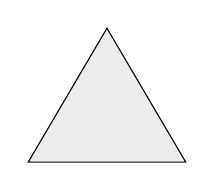
\begin{tikzpicture}
      \fill[gray!15] (0,0) -- (2,0) -- (1, 1.7) -- cycle;
      \draw (0,0) -- (2,0) -- (1, 1.7) -- cycle;
    \end{tikzpicture}
    \caption{$ \Delta_2 $}
  \end{subfigure}
  \begin{subfigure}{.33\textwidth}
    \centering
    \def\svgwidth{0.56\textwidth}
    \input{images/Tetrahedron.pdf_tex}
    \caption{$ \Delta_3 $}
  \end{subfigure}%
  \caption{Simplessi standard}
  \label{fig:lez1:standard_simplexes}
\end{figure}

\begin{definition}
  Dato uno spazio topologico $ X $ si definisce il \textbf{$ k $-simplesso singolare}\index{$ k $-simplesso singolare}
  in $ X $ come un'applicazione continua $ \sigma: \Delta_k \to X $.
\end{definition}
Spesso conviene identificare il $ k $-simplesso con la sua immagine in $ X $.
In questo modo uno $ 0 $-simplesso è un punto in $ X $, mentre un $ 1 $-simplesso singolare potrebbe
essere sia un segmento che un punto (se la mappa è costante).
Siccome non c'è relazione tra la dimensione dello spazio di partenza e lo spazio di arrivo
(ad esempio la curva di Peano) il simplesso può deformare, ed è per questo che è detto singolare.

\begin{example}
  Un esempio di $ k $-simplesso singolare in cui è particolarmente evidente la possibilità di fare l'identificazione
  è la mappa identità: $ \Id{} \colon \Delta_k \to \Delta_k $.
\end{example}
\begin{osservation}
  Quando è possibile faccio un abuso di notazione e identifico la mappa con la sua immagine
  nello spazio topologico.
\end{osservation}

Voglio costruire un complesso di gruppi abeliani e definire l'omologia singolare
come l'omologia di tale complesso.

\begin{definition}
  Si definisce lo spazio delle $ k $-\textbf{catene
    singolari}\index{$ k $-catene singolari} come il gruppo generato da tutte le
  possibili applicazioni continue da $ \Delta_k $ a $ X $, cioè:
  \[
    S_k(X) = \langle \set{g | g \text{ $ k $-simplesso singolare in $ X $}} \rangle
  \]
  Cioè:
  \begin{align*}
  S_k(X) ={}& \{\text{combinazioni lineari finite a coefficienti interi: } \\
            & \sum_g n_g g \;|\; n_g \in \Z, g \; k-\text{simplessi singolari di } X \}
  \end{align*}
\end{definition}
$ S_k(X) $ è un gruppo abeliano con l'operazione somma definita naturalmente:
\[
  \sum_g n_g g + \sum_h n_h h =   \sum_g n_g g + \sum_g n_g^\star g = \sum_g (n_g + n_g^\star)g
\]
Inoltre $ \forall k < 0 $ si pone $ S_k(X) = 0 $. Un elemento generico di $ S_k(X) $
è una somma formale finita (cioè con un numero finito di coefficienti non nulli)
su tutti i possibili $ k $-simplessi singolari in $ X $.
% \begin{example}
%   \[
%     (n_1 g_1 + n_2 g_2 + 2 n_3 g_3) + (m_1 g_1 + m_4 g_4) = (n_1 + m_1)g_1 + n_2 g_2 + 2 n_3 g_3 + m_4 g_4
%   \]
% \end{example}
Questa è una somma con tutte le giuste proprietà. Lo zero è la catena con tutti
i coefficienti nulli, mentre l'inverso è la catena con i coefficienti opposti.
Si nota che le catene sono somme formali di mappe e non sono esse stesse mappe.

\begin{example}[$ k = 0$]
  Se $ k = 0 $ allora $ S_0(X) $ sono catene di punti ($ g_0 : \Delta_0 \to X $,
  identifico l'applicazione con il punto in $ X $ sapendo che l'immagine di un
  punto è un punto)
  \[
    S_0(X) = \set { \sum n_i p_i | n_i \in \Z, \; p_i \in X}
  \]
\end{example}

A questo punto considero la successione $ S_\bullet $ ($ S $ sta per singolare), cioè:
\[
  \dots \to S_{k+1}(X) \to S_k(X) \to S_{k-1}(X) \to \dots \to S_0(X)
\]
Per rendere $ S_\bullet $ un complesso bisogna le applicazioni tra i vari
$ S_k $, queste applicazioni saranno il bordo. A questo scopo noto
$ h: \Delta_1 \to X $ è arco, e posso ottenere una $ 0 $-catena prendendo i punti
estremi dell'arco, infatti il bordo di un $ 1 $-simplesso è uno $ 0 $-simplesso.
L'idea è quindi ottenere simplessi di ordine più piccolo prendendo il bordo dei
simplessi. Questa operazione si generalizza con l'operatore faccia.

\begin{figure}[htbp]
  \centering
  \begin{tikzpicture}
    \draw[-Latex] (0,0) -- (2,0);
    \draw[-Latex] (0,0) -- (0,2);
    \draw[thick] (0,1) -- (1,0);
    \draw plot [smooth cycle] coordinates {(5,2) (6,3) (7,3) (6,0) (4,0)};
    \node () at (7,1) {$ X $};
    \draw plot [smooth, tension = 1] coordinates {(6,2) (5,1) (5.5,0.5)};
    \node[circle] () at (6,2) {\textbullet};
    \node[circle] () at (5.5,0.5) {\textbullet};
    \draw[->] (0.75,0.5) -- (4.75,1);
  \end{tikzpicture}
  \caption{1-Simplesso singolare}
  \label{fig:lez1:1_standard_simplex_with_arc}
\end{figure}

\begin{definition}
  Sia $ \Delta_k $ un $ k $-simplesso standard con $ k \geq 0 $ si definisce l'operatore \textbf{faccia}\index{Operatore faccia}
  come la mappa $ F_i^{\;k}: \Delta_{k-1} \to \Delta_k $ tale che $ F_i^{\;k}(\Delta_{k-1}) $ è una faccia di $ \Delta_k $.
\end{definition}
L'operatore faccia prende un $ k $-simplesso standard e lo immerge in un qualche senso in un
simplesso più grande, ad esempio manda un punto in uno degli estremi di un segmento (nel caso $ k = 0 $),

\begin{example}[$ k = 2 $]
  Per $ k = 2 $ vale che:
  \[
    \Delta_2 = \set{ (x_1,x_2,x_3) \in \RN{3} | x_1 + x_2 + x_3 = 1, \; 0 \leq x_i \leq 1 \; \forall i}
  \]
  Si definisce la base $ e_0 = (1,0,0) \; e_1 = (0,1,0) \; e_2 = (0,0,1) $, voglio vedere il bordo del triangolo
  come facce.

  \begin{figure}[htbp]
    \centering
    \begin{tikzpicture}
      \draw[-Latex] (0,0) -- (4,0);
      \draw[-Latex] (0,0) -- (0,4);
      \draw[-Latex] (0,0) -- (-2,-2);
      \node[below] () at (2,0) {$ e_1 $};
      \node[right] () at (0,2) {$ e_2 $};
      \node[right, below] () at (-1,-1) {$ e_0 $};
      \fill[gray!40, fill opacity=0.75] (-1, -1) -- (2,0) -- (0,2) -- cycle;
      \draw (-1,-1) -- (2,0);
      \draw (0,2) -- (2,0);
      \draw (0,2) -- (-1,-1);
      \fill[gray!15] (5,0) -- (9,0) -- (7,3) -- cycle;
      \draw (5,0) -- (9,0) -- (7,3) -- cycle;
      \node[left] () at (5,0) {$ e_0 $};
      \node[right] () at (9,0) {$ e_1 $};
      \node[above] () at (7,3) {$ e_2 $};
      \node[below] () at (7,0) {$ F_2^{(2)}(\Delta_1) $};
      \node[left] () at (6,2) {$ F_1^{(2)}(\Delta_1) $};
      \node[right] () at (8,2) {$ F_0^{(2)}(\Delta_1) $};
    \end{tikzpicture}
    \caption{Azione dell'operatore faccia}
    \label{fig:lez1:standard_simplex_faces}
  \end{figure}
\end{example}

Il segmento faccia $ i $-esimo è quello che non contiene il vertice $ i $-esimo, cioè
\emph{dimentico} un punto e gli altri punti diventano vertici del simplesso.

In generale se $ \Delta_k $ è un simplesso standard si definisce la base canonica come (si noti
che la base canonica è ordinata):
\begin{gather*}
  e_0 = (1,0,0,\dots)                            \\
  e_1 = (0,1,0,\dots)                            \\
  e_2 = (0,0,1,\dots)                            \\
  \dots
\end{gather*}
Questi sono i vertici del simplesso, definisco l'azione dell'operatore faccia
come:
\[
  \begin{cases}
    F_i^{\; k}(e_j) = e_{j+1}     & \text{se } j \geq i \\
    F_i^{\; k}(e_j) = e_{j} & \text{se } j < i
  \end{cases}
\]

% Se fosse un tetraedro dimenticando punti ottengo triangoli e dimenticando
% triangoli ottengo punti, come è giusto.

\begin{exercise}
  Dimostrare che se $ [\cdot, \cdot] $ indica l'inviluppo convesso allora:
  \begin{enumerate}
  \item Per $ j > i $ vale che $ F_j^{\; k+1} \circ F_i^{\; k} = [e_0, \dots, \hat{e}_i, \dots, \hat{e}_j, \dots, e_k ] $.
  \item Per $ j \leq i $ vale che $ F_j^{\; k+1} \circ F_i^{\; k} = [e_0, \dots, \hat{e}_j, \dots, \hat{e}_{i+1}, \dots, e_k ] $.
  \end{enumerate}
  dove i cappucci indicano che quell'elemento è omesso.
\end{exercise}

\begin{definition}
  L'\textbf{inviluppo convesso}\index{Inviluppo convesso} di un insieme $ U $ in
  $ \RN{n} $ è il più piccolo insieme convesso che contiene $ U $, dove un
  insieme in $ \RN{n} $ si dice \textbf{convesso}\index{Insieme convesso} se
  contiene il segmento che unisce ogni coppia di punti dell'insieme.
\end{definition}

\begin{definition}
  Dato un $ k $-simplesso singolare $ \sigma: \Delta_k \to X $ una sua faccia è data dalla
  mappa $ \sigma^{(i)} \colon \Delta_{k-1} \to X $ cioè la restrizione di
  $ \sigma $ sulla faccia $ i $-esima del simplesso, cioè
  $ \sigma^{(i)} = \sigma \circ F_i^{\; k} $, si definisce quindi il
  \textbf{bordo}\index{Bordo} come la mappa:
  \begin{align*}
    \partial \colon \Sigma_k(X) & \to \Sigma_{k-1}(X) \\
    \sigma & \mapsto  \sum_{i=0}^{k}(-)^i \sigma^{(i)}
  \end{align*}
  dove $ \Sigma_k(X) $ indica lo spazio dei $ k $-simplessi singolari di $ X $.
  % di $ \sigma $ come $ \partial_k \sigma = \sum_{i=0}^{k}(-)^i \sigma^{(i)} $.
\end{definition}
Il bordo sostanzialmente corrisponde alla somma alterna delle facce.

\begin{figure}[htbp]
  \centering
  \begin{tikzpicture}
    \draw[-Latex] (0,0) -- (3,0);
    \draw[-Latex] (0,0) -- (0,3);
    \draw[-Latex] (0,0) -- (-1.5,-1.5);
    \fill[gray!40, fill opacity=0.75] (-1, -1) -- (2,0) -- (0,2) -- cycle;
    \draw (-1,-1) -- (2,0);
    \draw (0,2) -- (2,0);
    \draw (0,2) -- (-1,-1);
    \draw plot [smooth cycle] coordinates {(5,2) (6,3) (7,3) (6.5,0) (4,0)};
    \node () at (7.5,1) {$ X $};
    \draw plot [smooth, tension = 1] coordinates {(6,2) (5,1) (5.5,0.5)};
    \draw plot [smooth, tension = 1] coordinates {(6,2) (6.2,0.7) (5.5,0.5)};
    \draw[->] (0.75,0.5) -- (4.75,1);
    \node[above] () at (2.5, 0.75) {$ \sigma $};
    \draw[->] (0.35,-0.65) to [out=-30,in=-120]  (5.35,0.45);
    \node () at (2.5, -1.45) {$ \sigma^{(i)} $};
  \end{tikzpicture}
  \caption{Azione di $ \sigma $ e $ \sigma^{(i)} $}
  \label{fig:lez1:sigma}
\end{figure}

\begin{example}[$ k = 1 $]
  Per $ k = 1 $ vale che $ \partial_1 \sigma = p_1 - p_0 $, infatti:
  \begin{align*}
    \sigma^{0} = \sigma \circ F_0^{\; 1} = \sigma(1) = p_1 \\
    \sigma^{1} = \sigma \circ F_1^{\; 1} = \sigma(0) = p_0
  \end{align*}
  Il bordo è la somma con i segni alternati: $ \partial_1 \sigma = p_1 - p_0 $. Tecnicamente
  il bordo è una mappa quindi sarebbe più corretto scrivere
  $ \partial_1 \sigma = \sigma^{(1)} - \sigma^{(0)} $ dove l'azione di queste due mappe è quella di
  mandare un estremo dell'intervallo $ [0,1] $ in $ p_0 $ o $ p_1 $.
\end{example}

Si è quindi definito il bordo sui simplessi singolari, ma si può generalizzare
la definizione sull'intero gruppo di catene
$ \partial_k: S_k(X) \to S_{k-1}(X) $ estendendo la definizione per linearità
$ \partial_k \left( \sum_g n_g g\right) = \sum_g n_g \partial_k g $, dove $ g $ sono simplessi
singolari, che sono i generatori di $ S $. A questo punto si
$ (S_\bullet, \partial) $ è una successione di gruppi abeliani, per mostrare che è un
complesso bisogna verificare che $ \partial_k $ è un omomorfismo e che
soddisfa $ \partial_k \circ \partial_{k+1} = 0 $.

\begin{proposition}
  La mappa $ \partial \colon S_k(X) \to S_{k-1}(X) $ è un omomorfismo.
\end{proposition}
\begin{proof}
  \begin{gather*}
    \partial_k \left( \sum_g n_g g + \sum_g m_g g\right) = \partial_k \left( \sum_g(m_g + n_g)g \right) = \sum_g (m_g + n_g) \partial_k g = \\
    = \sum_g n_g \partial_k g + \sum_g m_g \partial_k g = \partial_k \left( \sum_g n_g g\right) + \partial_k \left( \sum_g m_g g \right)
  \end{gather*}
  Dove si è usato che la mappa di bordo è lineare.
\end{proof}
\hfill \newline \newline \noindent
Una volta verificato che $ \partial_k \circ \partial_{k+1} = 0 $ (spesso come notazione si pone $ \partial^2 = 0 $)
il complesso sarà:
\[
  \begin{tikzcd}
    \dots \rar & S_{k+1}(X) \arrow{r}{\partial_{k+1}} & S_k(X) \arrow{r}{\partial_k} & S_{k-1}(X) \arrow{r}{\partial_{k-1}} & \dots
  \end{tikzcd}
\]
\vspace*{-12pt}
\begin{proposition}
  Vale che $ \partial_k \circ \partial_{k+1} = 0 $.
\end{proposition}
\begin{proof}
  È sufficiente verificare la proprietà sui generatori, quindi se $ \sigma $ è un
  $ k $-complesso singolare, cioè $ \sigma : \Delta_k \to X $ continua:
  \begin{gather*}
    \partial_k \circ \partial_{k+1} \sigma = \partial_k \left( \sum_{j=0}^{k+1}(-)^j (\sigma \circ F_j^{\; k+1}) \right) =  \sum_{j=0}^{k+1}(-)^j \partial_k (\sigma \circ F_j^{\; k+1}) = \\
    = \sum_{j=0}^{k+1} (-)^j \sum_{i=0}^k (-)^i (\sigma \circ F_j^{\; k+1}) \circ F_i^{\; k} = \sum_{j = 0}^{k+1} \sum_{i = 0}^{k} (-)^{j+i} \sigma \circ F_j^{\; k+1} \circ F_{i}^{\; k} =
  \end{gather*}
  Separo le somme con $ i < j $ e quelle con $ i \geq j $:
  \[
    = \sum_{0 \leq i < j \leq k + 1} (-)^{i+j} \sigma \circ F_j^{\; k+1} \circ F_i^{\; k} + \sum_{0 \leq j \leq i \leq k} (-)^{i+j} \sigma \circ F_j^{\; k+1} \circ F_i^k =
  \]
  Usando la proprietà degli inviluppi convessi si trova che se $ j \leq i $ allora
  $ F_j^{\; k+1} \circ F_j^{\; k} = F_{i+1}^{\; k+1} \circ F_k^{k} $, infatti se
  $ j \leq i $ allora $ i + 1 \geq j $ quindi in entrambi i membri l'inviluppo convesso è
  $ [e_0, \dots \hat{e}_j, \dots, \hat{e}_{i+1}, \dots, e_k] $. Quindi:
  \[
    = \sum_{0 \leq i < j \leq k + 1} (-)^{i+j} \sigma \circ F_j^{\; k+1} \circ F_i^{\; k} + \sum_{0 \leq j < i \leq k} (-)^{i+j} \sigma \circ F_{i+1}^{\; k+1} \circ F_j^{\; k}  =  0
  \]
  Dove nell'ultimo si è rinominato nel secondo termine $ i + 1 $ con $ i $, e ciò produce un segno
  meno che annulla la somma.
  % Si nota che è di importanza cruciale il fatto che si è definito il bordo con i
  % segni alternati.
\end{proof}

% lezione 2
% _     _____ ________ ___  _   _ _____   ____
% | |   | ____|__  /_ _/ _ \| \ | | ____| |___ \
% | |   |  _|   / / | | | | |  \| |  _|     __) |
% | |___| |___ / /_ | | |_| | |\  | |___   / __/
% |_____|_____/____|___\___/|_| \_|_____| |_____|


% Sia $ X $ uno spazio topologico, voglio definire l'omologia singolare $ H_k(X) $, cioè il $ k $-esimo gruppo di omologia
% singolare. Costruisco il complesso $ (S_\bullet(X), \partial) $ con:
% \[
%   S_k(X) = \set{ \sum_g n_g g | g \text{ simplesso singolare, } n_g \in \Z }
% \]
% E $ \partial_k : S_k(X) \to S_{k-1}(X) $ applicazione di bordo con $ \partial_k(g) = \sum_{i=0}^k(-)^ig^{(i)} $ con $ g: \Delta_k \to X $, e poi lo estendo per
% linearità su tutti gli elementi di $ S $, dove $ g^{(i)} = g \circ F_i^{\; k} $.

% Siccome $ \partial_{k-1} \circ \partial_k = 0 $ si ha il complesso
% \[
%   \begin{tikzcd}
%     \dots \arrow{r}{\partial_{k+1}} & S_k(X) \arrow{r}{\partial_k} & S_{k-1}(X) \arrow{r}{\partial_{k-1}} & \dots
%   \end{tikzcd}
% \]
% Inoltre $ \partial_k \circ \partial_{k-1} $ è la mappa nulla dalle catene singolari di $ S_k(X) $
% a quelle di $ S_{k-2}(X) $, in questo modo $ (S_\bullet(X), \partial) $ è un complesso di gruppi abeliani.

\section{Omologia singolare}

\begin{definition}
  Si definisce l'\textbf{omologia singolare}\index{Omologia singolare} $ H_k(X) $ dello spazio topologico $ X $
  come l'omologia del complesso $ (S_\bullet(X),\partial) $, cioè:
  \[
    H_k(X) := H_k(S_\bullet(X)) = \quot{\ker{\partial_k}}{\im{\partial_{k+1}}}
  \]
\end{definition}
% Posso quindi calcolare l'omologia di $ (S_\bullet(X),\partial) $ come l'avevo definita
% in precedenza:
% \[
%   H_k(S_\bullet(X)) = \quot{\ker{\partial_k}}{\im{\partial_{k+1}}}
% \]
% Vale che $ \ker{\partial_k} = \set{c \in S_k(X) | \partial_k(c) = 0} $, cioè le $ k $-catene con
% bordo nullo, questi sono chiamati $ k $-cicli.

\begin{definition}
  Sia $ (S_\bullet(X),\partial) $ un complesso di moduli, gli elementi di $ \ker{\partial_k} $ sono detti
  \textbf{$ k $-cicli}\index{$ k $-ciclo}. Un $ k $-ciclo è quindi una $ k $-catena
  con bordo nullo:
  \[
    c \text{ ciclo } \Leftrightarrow \partial c = 0
  \]
  L'insieme dei $ k $-cicli è indicato con $ Z_k(X) $, cioè: $ Z_k(X) = \ker{\partial_k} $.
  Si indica invece con $ B_k(X) $ l'insieme dei \textbf{bordi}\index{$ k $-bordo}, cioè le $ k $-catene singolari
  che sono immagini di $ k+1 $-catene, cioè esplicitamente:
  \[
    B_k(X) = \set{\eta \in S_k(X) | \exists b \in S_{k+1}(X), \partial b = \eta}
  \]
\end{definition}
Per definizione si ha quindi che $ H_k(X) = {Z_k(X)} \slash {B_k(X)} $, cioè il
gruppo di omologia è formato dai cicli modulo i bordi. Esplicitamente gli
elementi di $ H_k(X) $ sono classi di equivalenza tali che se $ \llbracket c \rrbracket \in H_k(X) $
con $ \partial c = 0 $ e $ c_1 \in  \llbracket c \rrbracket  $ allora $ c_1 - c \in B_k(X) $ e
$ \partial c_1 = 0 $ quindi esiste $ b $ tale che $ c_1 - c = \partial b $. Cioè due elementi
stanno nella stessa classe di equivalenza se differiscono per un bordo:

\newmathsymb{homolog}{\sim_{hom}}{Relazione di omologia}
\begin{definition}
  Due elementi $ a,b $ si dicono \textbf{omologhi} \index{Elementi omologhi} se differiscono per un bordo.
  \[
    a \sim_{hom} b \Leftrightarrow \exists c \; | \; \partial_k c = a - b
  \]
\end{definition}

\begin{osservation}
  Vale che $ H_k(X) = 0 $ se e solo se $ B_k(X) = Z_k(X) $, cioè se ogni ciclo è
  un bordo, come si è già osservato. In generale si ha che
  $ B_k(X) \subseteq Z_k(X) $ e possono esserci cicli che non sono immagini di bordi.
\end{osservation}
% $ \partial_k c $ è il bordo di un $ k $-ciclo, se $ \partial_k c = 0 $ significa che il ciclo non ha bordo, inoltre
% se $ c = \partial_{k+1} b $ allora $ c $ è bordo di qualcosa: $ c $ è un bordo che non ha bordo. Questo tipo
% di oggetti è di interesse centrale
Scopo del corso è studiare $ H_k(X) $ e capire se si possono determinare a meno
di isomorfismi, quello che si trova è In alcuni casi è possibile calcolare
esplicitamente i gruppi di omologia, come nel caso dell'omologia cellulare.

\subsection{$ H_0(X) $}

\begin{proposition}
  Sia $ X $ uno spazio topologico connesso per archi, allora $ H_0 \cong \Z $, cioè è uno $ \Z $-modulo libero di rango 1.
  In effetti $ H_0(X) $ \emph{conta} le componenti connesse per archi in $ X $ e quindi dà informazioni di natura geometrica.
\end{proposition}
\begin{proof}
  Calcolo $ H_0 $ a partire dalla definizione di omologia:
  \[
    H_0(X) = \quot{Z_0(X)}{B_0(X)}
  \]
  Ho il complesso:
  \[
    \begin{tikzcd}
      \dots \arrow{r}{} & S_1(X) \arrow{r}{\partial_1} & S_0(X) \arrow{r}{\partial_0}  & 0
    \end{tikzcd}
  \]
  Quindi $ Z_0 = \ker{\partial_0} = S_0(X) $ in quanto ogni elemento di $ S_0(X) $ viene
  mandato in $ 0 $.

  % Ma $ Z_0(X) = \set{ c \in S_o(X) | \partial_0 c = 0} $ e $ S_0(X) = \set{ \sum n_i p_i | n_i \in \mathbb{N}, p_i \in X} $.
  % % Tecnicamente uno $ 0 $-simplesso singolare è una mappa $ \sigma_0 : \Delta_0 \to X $ tale che manda $ \Delta_0 = 1 $ in $ \sigma_0(1) = p_0 $ e per
  % % questo è naturale l'identificazione con i punti immagine dello spazio topologico.
  % Sia $ c \in S_0(X) $ allora $ c = \sum n_i p_i $, e vale che $ \partial_0(c) = \sum n_i \partial_0 (p_i) = 0 $, infatti
  % $ \partial_0 : S_0(X) \to S_{-1}(X) $, ma per $ k < 0 $ $ S_{k} = 0 $ per definizione.
  Quindi per ora ho che:
  \[
    Z_0(X) = \ker{\partial_0} = S_0(X) \; \Rightarrow \; H_0(X) = \quot{S_0(X)}{B_0(X)}
  \]
  Per definizione
  $ B_0(X) = \im{\partial_1} = \set{ x \in S_0(X) | \exists \alpha \in S_1(X), \; \partial_1(\alpha) = x}
  $. % $ \alpha $ è una catena.
  Ma $ S_0(X) $ è il gruppo libero generato dagli $ 0 $-simplessi singolari, che
  sono mappe $ \Delta_0 \to X $, e siccome $ \Delta_0 $ è un punto si possono identificare
  con i punti di $ X $, perciò si può immaginare formalmente $ S_0(X) $ come il
  gruppo libero generato dai punti di $ X $. $ B_0(X) $ è l'insieme delle coppie
  di punti di $ X $ che sono bordo di un $ 1 $-simplesso singolare, il quale è
  una mappa $ \Delta_1 \cong I \to X $, cioè è un arco. Siccome lo spazio è connesso per
  archi ogni coppia di punti è bordo di qualcosa, fissando un punto $ x \in X $
  sostanzialmente $ B_0(X) $ lo si può immaginare come $ X $ stesso e quindi
  $ H_0(X) \cong \Z $ in quanto quoziente tra un gruppo libero generato da un
  insieme di punti e l'insieme di punti stessi, quindi esiste un'unica classe di
  equivalenza che è quella di un punto, in quanto ogni coppia di punti è omologa
  essendo collegata da un arco.

  Se ci sono più componenti connesse per archi posso ripetere il ragionamento senza connettere componenti
  distinte, quindi trovo che:
  \[
    H_0(X) \cong \Z^{N_c}
  \]
  Dove $ N_c $ è il numero di componenti connesse per archi di $ X $ con
  $ N_c < + \infty $, in pratica $ H_0(X) $ è generato da un insieme formato da un
  punto per ogni componente connessa per archi.
  % Se $ X $ non è connesso per archi ma è composto da diverse componenti connesse
  % per archi allora si può applicare il precedente ragionamento per ciascuna
  % componente, e quindi si otterrebbe $ \Z^n $ dove $ n $ e il numero di
  % componenti.
  %
  % Per questo $ H_0 (X) \cong \Z $ generato dalla classe $ [p] \; \forall p \in X $ (con $ X $ connesso per archi).
  % Sia $ p_0 \in X $, allora $ q \sim_{hom} p_0 $ se e solo se $ \exists \alpha \in S_1(X) $ tale che $ q - p_0 = \partial_1 \alpha $.
  % Per questo motivo i punti sono tutti omologhi, infatti
  % essendo $ X $ connesso per archi esiste un arco $ \alpha $ che connette $ q $ e $ p_0 $, ma
  % per definizione gli archi sono applicazioni continue da $ \Delta_1 $ a $ X $ che hanno come bordo $ q - p_0 $.
  % Esiste quindi un'unica classe di equivalenza che è la classe di equivalenza di un punto.
  % Per questo il gruppo è omomorfo a $ \Z $.
\end{proof}
\hfill\newline\newline \noindent
La mappa che realizza questo isomorfismo è nota come grado.
\begin{definition}
  Si definisce la mappa \textbf{grado} \index{Grado} come l'applicazione che manda una catena in $ S_0(X) $ nella somma
  dei suoi coefficienti:
  \begin{align*}
    \deg \colon S_0(X)    & \to  \Z \\
    \sum n_i p_i & \mapsto  \sum n_i
  \end{align*}
\end{definition}

\begin{proposition}
  La mappa grado gode di alcune proprietà:
  \begin{enumerate}
  \item $ \deg $ è un omomorfismo di gruppi abeliani
  \item $ \deg $ è suriettivo
  \item $ \ker{\deg} \cong B_0(X) $
  \end{enumerate}
  Se dimostro questa proprietà utilizando il primo teorema fondamentale di isomorfismo:
  \[
    \quot{S_0(X)}{B_0(X)} \cong \im{\deg}
  \]
  Ma $ \deg $ è suriettiva, quindi $ \im{\deg} = \Z $, perciò:
  \[
    H_0(X) = \quot{S_0(X)}{B_0(X)} \cong \Z
  \]
\end{proposition}
Dimostro quindi questa proposizione. \\
\begin{proof}
  \begin{enumerate}
  \item
    Sia $ c_1 = \sum n_i p_i $ e $ c_2 = \sum m_i q_i $, bisogna mostrare che:
    \[
      \deg(c_1 + c_2) = \deg(c_1) + \deg(c_2)
    \]
    ma:
    \[
      c_1 + c_2 = \sum n_i p_i + \sum m_i q_i = \sum (n_i + m_i)r_i
    \]
    dove $ r_i $ è quello comune tra le catene, oppure è zero se
    l'elemento è presente in solo uno delle due catene.
    Quindi:
    \[
      \deg(c_1 + c_2) = \sum (n_i + m_i) = \sum n_i + \sum m_i = \deg(c_1) + \deg(c_2)
    \]
    Alternativamente in modo più semplice si può osservare l'azione di $ \deg $
    sui generatori di $ S_0(X) $, il quale possiede un solo generatore che viene
    mandato dalla mappa grado in $ 1 $, quindi si estende per linearità.
  \item
    La mappa è suriettiva, è sufficiente prendere un punto $ p \in X $
    e la controimmagine di $ m \in \Z $ è $ \deg^{-1}(m) = mp $
  \item
    Mostro che $ \ker{\deg} = B_0(X) $, e lo faccio msotrando che $ \ker{\deg} \subseteq B_0(X) $
    e che  $ \ker{\deg} \supseteq B_0(X) $.

    Inizio con $ \ker{\deg} \subseteq B_0(X) $: sia $ c \in \ker{\deg} $ cioè tale che $ \deg(c) = 0 $,
    se $ c = \sum n_i p_i $ allora $ \sum n_i = 0 $, voglio mostrare che $ c \in B_0(X) $,
    cioè che $ \exists b \in S_1(X) $ con $ \partial_1 b = c $.

    Fissato $ p_0 $ considero i $ p_i $, ci sono archi
    $ \lambda_i $ che li uniscono a $ p_0 $. $ b $ si può costruire in questo modo: siano
    $ \lambda_i : [0,1] \to X $ con $ \lambda_i(0) = p_0 $ e $ \lambda_i(1) = p_i $ allora:
    \begin{gather*}
      c - \partial\left(\sum n_i \lambda_i \right) =  c - \sum n_i \partial \lambda_i = c - \sum n_i (p_i - p_0) = \\
      = c - \sum n_i p_i
      + \sum n_i p_0 = p_0 \sum n_i = 0
    \end{gather*}
    In cui si è usato che per ipotesi $ c \in \ker{\deg} $ quindi $ \sum n_i = 0 $ e che $ c = \sum n_i p_i  $.
    Ma quindi $ c = \partial(\sum n_i \lambda_i) $ e definendo $ \sum n_i \lambda_i = b $ si è trovato l'elemento $ b $,
    per cui $ \ker{\deg} \subseteq B_0(X) $.

    Mi rimane da mostrare che $ B_0(X) \subseteq \ker{\deg} $: mostro che se $ c \in B_0(X) $ allora
    $ c \in \ker{\deg} $, cioè, $ \deg(c) = 0 $.
    Siccome $ c \in B_0(X) $ esiste $ b \in S_1(X) $ tale che $ c = \partial b $, ma $ S_1(X) $
    è lo spazio generato dagli $ 1 $-simplessi singolari, cioè dagli archi, quindi
    chiamando $ \lambda_i $ gli archi si può scrivere $ b = \sum m_i \lambda_i $.
    A questo punto:
    \[
      \deg(c) = \deg(\partial b) = \sum n_i \deg(\partial \lambda_i) = 0
    \]
    In quando $ \partial \lambda_i = \lambda_i(1) - \lambda_i(0) $ e l'azione dell'opertaore grado è quella di sommare i coefficienti,
    che sono opposti.

    Siccome $ \ker{\deg} = B_0(X) $ in particolare gli spazi sono isomorfi.
  \end{enumerate}
  Per questo si può utlizzare il primo teorema dell'isomorfismo, come indicato
  all'inizio di questa dimostrazione.
\end{proof}
% \hfill \newline\newline

\subsection{$ H_1(X) $}
% lezione 3 parte 2

% Cosa si può dire invece su $ H_1(X) $?

Sia $ X $ spazio topologico e $ x_0 \in X $, alla coppia $ (X, x_0) $ si associa
il gruppo fondamentale $ \pi_1(X,x_0) $, il quale in generale non è abeliano. Per
questo motivo conviene studiare la versione abelianizzata:
$ \Ab{\pi_1(X,x_0)} = {\pi_1(X,x_0)} \slash {\pi_1(X,x_0)'} $ dove $ ' $ indica il
  \textbf{gruppo derivato}\index{Gruppo derivato}, cioè il gruppo generato dai
  commutatori.
\[
  \pi_1(X,x_0)' = [\pi_1(X,x_0), \pi_1(X,x_0)] = \langle\set{[g,h] | g,h \in \pi_1(X,x_0)}\rangle
\]
Il gruppo derivato è il gruppo dei prodotti formali di elementi del tipo
$ aba^{-1}b^{-1} $, quando passo al quoziente questi oggetti si annullano e
quindi $ ab = ba $ (infatti
$ aba^{-1}b^{-1} = 1 \Rightarrow aba^{-1} = b \Rightarrow ab = ba $), per questo si ottiene il
gruppo abelianizzato.

Se $ X $ è connesso per archi allora mostrerò che $ \Ab{\pi_1(X,x_0)} \cong H_1(X) $,
quindi conoscendo il gruppo fondamentale si può calcolare anche
il primo gruppo di omologia, che quindi è sostanzialmente formato dai lacci
(modulo omotopia) che commutano tra loro.

% lezione 3 parte 2

\begin{osservation}
  Sia $ X $ uno spazio topologico connesso per archi e $ \mathcal{G} $ un gruppo
  abeliano se esiste un omomorfismo di gruppi $ \phi: \pi_1(X) \to \mathcal{G} $ allora
  esiste $ \phi' : \Ab{\pi_1(X)} \to \mathcal{G} $ omomorfismo di gruppi abeliani.
  \[
    \begin{tikzcd}
      \pi_1(X) \arrow{r}{\phi} \arrow{d}{P} & \mathcal{G} \\
      \Ab{\pi_1(X)} \arrow{ur}{\phi'}
    \end{tikzcd}
  \]
  dove $ P $ è la proiezione sul quoziente.
\end{osservation}
\begin{proof}
  La definizione di $ \phi' $ è naturale, questa è tale che
  $ \phi'(P(c)) = \phi(c) $, ma bisogna controllare se questa è ben definita, cioè se
  prendendo rappresentanti equivalenti si ottengono le stesse immagini, cioè se
  considerati $ c \sim_H d $ risulta che $ \phi(c) = \phi(d) $. Se
  $ c \sim_H d $ allora $ P(c) = P(d) $, e quindi $ c = d[x,y] $ per opportuni
  $ x $ e $ y $, in quanto gli elementi in $ \Ab{\pi_1(X)} $ differiscono per
  commutatori. Applicando $ \phi $ si ottiene $ \phi(c) = \phi(d[x,y]) $, siccome
  $ \phi $ è omomorfismo:
  \[
    \phi(d[x,y]) = \phi(d)\phi([x,y]) = \phi(d) \phi(xyx^{-1}y^{-1}) = \phi(d) \phi(x) \phi(y) \phi(x)^{-1} \phi(y)^{-1} = \phi(d)
  \]
  dove nell'ultimo passaggio ho utilizzato che il gruppo è abeliano.
  Si nota che questa osservazione dipende crucialmente dal fatto che il gruppo è abeliano.
\end{proof}
\eproof
Per dimostrare che $ \Ab{\pi_1(X)} \cong H_1(X) $ mi serve prima un lemma:
\begin{lemma}
  Se $ f \sim_H g $ allora $ f \sim_{hom} g $, cioè se $ f $ e $ g $ sono lacci che
  definiscono lo stesso elemento nel gruppo fondamentale allora differiscono per
  un bordo ($ f \sim_H g \Rightarrow f \sim_{hom} g $).
\end{lemma}
\begin{proof}
  Siccome $ f \sim_{H} g $ allora $ \exists F $ continua tale $ F: I \times I \to X $ tale che $ F(0,x) = f(x) $,
  $ F(1,x) = g(x) $ e $ F(t,0) = F(t, 1) = x_0 $.
  Voglio mostrare che $ f - g $ è bordo di un $ 2 $-simplesso.
  Identificando tutti i punti di un uno dei due intervalli con l'equivalenza $ {I \times I} \slash {\set{0} \times I} $
  si ottiene qualcosa che è omeomorfo a $ \Delta_2 $, $ F $ sullo spigolo $ \set{0} \times I $
  assume sempre lo stesso valore.
  \begin{figure}[htb]
    \centering
    \begin{subfigure}[t]{1.0\linewidth}
      \centering
      \begin{tikzpicture}
        \draw (0, 0) rectangle (3,3);
        \draw[-Latex] (-0.5, 1) -- (-0.5, 2);
        \draw[-Latex] (1, -0.5) -- (2, -0.5);
        \node[left] () at (-0.5, 1.5) {$ t $};
        \node[below] () at (1.5, -0.5) {$ x $};
        \node[right] () at (0, 1.5) {$ C_{x_0} $};
        \node[left] () at (3, 1.5) {$ C_{x_0} $};
        \node[above] () at (1.5, 0) {$ f(x) $};
        \node[below] () at (1.5, 3) {$ g(x) $};
        \draw (0,2) -- (3,2);
        \draw[-Latex] (0, 2) -- (1.5, 2);
        \node[below] () at (1.5, 2) {$ F(t,x) $};
      \end{tikzpicture}
      \subcaption{Omotopia: deforma $ f $ in $ g $ in modo continuo.}
      \label{fig:lez3:homotopy_f_g}
    \end{subfigure}
    \begin{subfigure}[t]{1.0\linewidth}
      \centering
      \begin{tikzpicture}
        \draw (0, 0) rectangle (3,3);
        \fill[gray!15] (0, 0) rectangle (3,3);
        \draw[ultra thick] (3,0) -- (3,3);
        % \node[right] () at (0, 1.5) {$ C_{x_0} $};
        % \node[left] () at (3, 1.5) {$ C_{x_0} $};
        \node[above] () at (1.5, 0) {$ f(x) $};
        \node[below] () at (1.5, 3) {$ g(x) $};
        \draw[-Latex] (4,1.5) -- (5,1.5);
        \fill[gray!15] (6,0) -- (6, 3) -- (8.5,1.5) -- cycle;
        % \fill[gray!15] (6,0) -- (7.7, 3) -- (9.4,0) -- cycle;
        \draw (6,0) -- (6, 3) -- (8.5,1.5) -- cycle;
        % \draw (6,0) -- (7.7, 3) -- (9.4,0) -- cycle;
        \node[above, rotate = -30] () at (7.3, 2.2) {$ g(x) $};
        % \node[above, rotate = 60] () at (6.7, 1.3) {$ g(x) $};
        \node[above, rotate = 90] () at (6,1.5) {$ K(x) = C_{x_0} $};
        % \node[above, rotate = -58] () at (8.7, 1.3) {$ K(x) = C_{x_0} $};
        \node[rotate = 30] () at (7.3, 0.45) {$ f(x) $};
        % \node[below] () at (7.7, 0) {$ f(x) $};
        % \node[left] () at (6,0) {$ e_0 $};
        \node[right] () at (8.5,1.5) {$ e_0 $};
        \node[] () at (8.5,1.5) {$ \bullet $};
        % \node[] () at (6,0) {$ \bullet $};
        % \node[right] () at (9.4,0) {$ e_1 $};
        \node[below] () at (6,0) {$ e_1 $};
        % \node[above] () at (7.7,3) {$ e_2 $};
        \node[above] () at (6,3) {$ e_2 $};
      \end{tikzpicture}
      \subcaption{La relazione di equivalenza fa passare da un quadrato a un triangolo
        in quanto fa collassare un intervallo nel punto $ e_0 $. La rappresentazione
      non è fedele in quanto in effetti $ e_0 $ è il punto $ (1,0) $.}
      \label{fig:lez3:homotopy_f_g_to_triangle}
    \end{subfigure}
  \end{figure}
  [NON VA BENE, SISTEMARE!]
  Siccome $ F $ rimane costante sul sottospazio su cui su quozienta,
  dove vale sempre $ x_0 $,
  $ F $ induce $ F' \colon \Delta_2 \to X $ continua in cui $ e_0 $ viene mandato in $ x_0 $:
  \[
    \begin{tikzcd}
      I \times I \arrow{r}{F} \arrow{d}{P} & X \\
      \quot{I \times I}{\set{0} \times I} \simeq \Delta_2 \arrow{ur}{F'}
    \end{tikzcd}
  \]
  Calcolo il bordo: $ \partial F' = F'^{(0)} - F'^{(1)} + F'^{(2)} = K - g + f $
  dove $ K $ è il cammino costante per definizione di omotopia, cioè è
  $ C_{x_0}$. Se $ K $ fosse il bordo di qualcosa avrei finito, ma $ K $ è il
  $ 2 $-simplesso singolare costante uguale a $ x_0 $, cioè
  $ K \colon \Delta_2 \to \set{x_0} $, quindi il suo bordo:
  \[
    \partial K = K^{(0)} - K^{(1)} + K^{(2)} =  K^{(2)}
  \]
  in quanto tutti i tre termini sono uguali a $ k \colon \Delta_1 \to \set{x_0} $, quindi $ \partial K = K^{(2)} = k $,
  cioè $ k $ è un bordo, perciò:
  \[
    \partial F' = \partial k - F'^{(1)} + F'^{(2)} \Rightarrow \partial F' - \partial k = f - g \Rightarrow \partial(F' - k) = f - g
  \]
  $ F' - k $ è $ 2 $-simplesso singolare, lo chiamo $ \sigma $ ed è tale che $ \partial \sigma = f - g $, quindi
  $ f $ e $ g $ sono omologhi e $ \sigma $ è il $ 2 $-simplesso singolare che realizza
  l'omologia.
\end{proof}

\begin{proposition}
  Se $ X $ è uno spazio topologico allora esiste un omomorfismo ben definito
  $ \phi \colon \Ab{\pi_1(X)} \to H_1(X) $.
  % cioè si può passare dall'equivalenza  omologica a quella omotopica.
\end{proposition}
\begin{proof}
  Per dimostrare che $ \Ab{\pi_1(X, x_0)} \cong H_1(X) $ trovo un omomorfismo di
  gruppi abeliani tra $ \pi_1(X, x_0 $ a $ H_1(X) $, infatti
  se costruisco $ \phi \colon \pi_1(X, x_0) \to H_1(X) $ omomorfismo di gruppi ottengo
  gratuitamente la mappa da $ \Ab{\pi_1(X, x_0)} $ a $ H_1(X) $ per l'osservazione precedente.
  \[
    \begin{tikzcd}
      \pi_1(X, x_0) \arrow{r}{\phi} \arrow{d}{P} & H_1(X) \\
      \Ab{\pi_1(X, x_0)} \arrow{ur}{\phi'}
    \end{tikzcd}
  \]
  % Poi dovrò mostrare che questa mappa è invertibile, cioè $ \exists \psi:H_1(X) \to A_1(X) $ tale che $ \phi' \circ \psi = \Id{H_1(X)} $ e
  % $ \psi \circ \phi' = \Id{\Ab{\pi_1(X)}} $.
  Una possibile costruzione di $ \phi $ è:
  \begin{align*}
    \phi:  \pi_1(X, x_0) & \to H_1(X) \\
    [f]_H & \mapsto [f]_{hom} = \llbracket f \rrbracket
  \end{align*}
  % In tutto ciò non ho ancora utilizzato la connessione per archi.
  % Ora voglio costruire $ \phi' \colon \Ab{\pi_1(X)} \to H_1(X) $ e lo faccio ancora
  % senza l'ipotesi di connessione per archi.
  Per il lemma precedente questa applicazione è ben definita, bisogna mostrare
  che $ \phi $ è omomorfismo, e in questo modo anche
  $ \phi' \colon \Ab{\pi_1(X,x_0)} \to H_1(X) $ lo è. Siano
  $ [f]_H, [g]_H \in \pi_1(X, x_0) $ voglio fare vedere che:
  \[
    \phi ( [f]_H [g]_H) = \phi([f]_H) + \phi([g]_H)
  \]
  Questo è verso se e solo se:
  \[
    \phi([f \star g]_H) = [f]_{hom} + [g]_{hom}
  \]
  Che è vera se e solo se:
  \[
    [f \star g]_{hom} = [f + g]_{hom}
  \]
  Questo è vero se e solo se i due rappresentati sono equivalenti, cioè se
  differiscono per un bordo, ovvero se:
  \[
    \exists T: \Delta_2 \to X \text{ $ 2 $-simplesso singolare tale che } \partial T = f + g - f \star g
  \]
  Cioè:
  \[
    \partial T = T^{(0)} - T^{(1)} + T^{(2)} = f + g - f \star g
  \]
  \begin{figure}[htbp]
    \centering
    \begin{subfigure}[htbp]{.45\linewidth}
      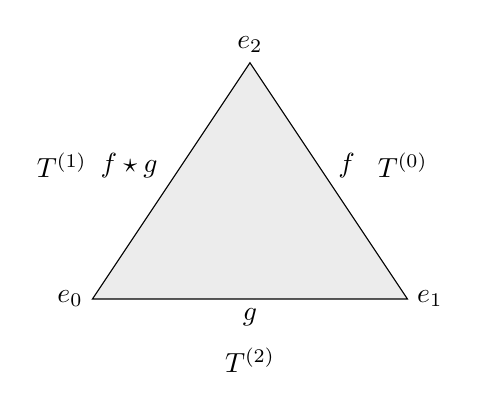
\begin{tikzpicture}
        \fill[gray!15] (5,0) -- (9,0) -- (7,3) -- cycle;
        \draw (5,0) -- (9,0) -- (7,3) -- cycle;
        \node[left] () at (5,0) {$ e_0 $};
        \node[right] () at (9,0) {$ e_1 $};
        \node[above] () at (7,3) {$ e_2 $};
        \node[below] () at (7,0) {$ g $};
        \node[below] () at (7,-0.5) {$ T^{(2)} $};
        \node[left] () at (5.95,1.7) {$ f \star g $};
        \node[left] () at (5.05,1.7) {$ T^{(1)} $};
        \node[left] () at (6.2,1.5) {};
        \node[right] () at (8,1.7) {$ f $};
        \node[right] () at (8.5, 1.7) {$ T^{(0)} $};
      \end{tikzpicture}
      \caption{Costruzione dell'omomorfismo}
      \label{fig:lez3:proof_homo_1}
    \end{subfigure}
    \begin{subfigure}[htbp]{.45\linewidth}
      \centering
      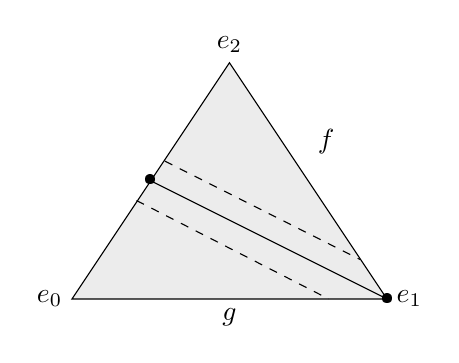
\begin{tikzpicture}
        \fill[gray!15] (5,0) -- (9,0) -- (7,3) -- cycle;
        \draw (5,0) -- (9,0) -- (7,3) -- cycle;
        \node[left] () at (5,0) {$ e_0 $};
        \node[right] () at (9,0) {$ e_1 $};
        \node[above] () at (7,3) {$ e_2 $};
        \node[below] () at (7,0) {$ g $};
        % \node[left, above] () at (5.95,1.7) {$ f \star g $};
        % \node[left] () at (5.9,1.5) {$ \frac{1}{2} $};
        \node[] (n1) at (6.,1.5) {\textbullet};
        \node[] (n2) at (9,0) {\textbullet};
        \node[right] () at (8,2) {$ f $};
        \draw (6,1.5) -- (9,0);
        \draw[dashed] (6.18,1.75) -- (8.66, 0.5);
        \draw[dashed] (5.82,1.25) -- (8.26, 0);
      \end{tikzpicture}
      \caption{Costruzione dell'omomorfismo, deve avere valori costanti su rette parallele}
      \label{fig:lez3:proof_homo}
    \end{subfigure}
    \caption{Costruzione dell'omomorfismo}
  \end{figure}
  Una possibile costruzione di $ T $ consiste mettere $ g $ su lato $ e_0 e_1 $,
  $ f $ sul lato $ e_1 e_2 $ e poi definire $ T \colon \Delta_2 \to X $ in modo che all'interno
  del simplesso abbia valori determinati dall'intersezione di rette parallele alla
  retta che divide il lato $ e_2 e_1 $ in due (cioè la mediana) con gli altri due
  lati del simplesso. In questo modo su metà del terzo lato c'è esattamente $ f $,
  e sull'altra metà $ g $, cioè complessivamente $ f \star g $.
\end{proof}
\hfill \newline \newline \noindent La mappa $ \phi: \pi_1(X,x_0) \to H_1(X) $ è un omomorfismo di
gruppi ben definito anche se $ X $ non è connesso per archi, e dato che
$ H_1(X) $ è abeliano per il precedente lemma è ben definito
$ \phi': \Ab{\pi_1(X)} \to H_1(X) $ omomorfismo di gruppi abeliani. Richiedendo che
$ X $ sia anche connesso per archi si ottiene che $ \phi' $ è un isomorfismo, come
afferma il \textbf{teorema di Hurewicz}.
\begin{theorem}[Teorema di Hurewicz\index{Teorema di Hurewicz}]
  Se $ X $ è uno spazio topologico
  connesso per archi allora  $ \phi \colon \Ab{\pi_1(X)} \to H_1(X) $
  è un isomorfismo, quindi $ \Ab{\pi_1(X)} \cong H_1(X) $.
\end{theorem}
\begin{proof}
  \emph{Sketch of proof, la dimostrazione completa è piuttosto noiosa}. Per
  dimostrare che $ \phi' $ è isomorfismo mostro che è invertibile,
  $ \exists \psi \colon H_1(X) \to \Ab{\pi_1(X)} $ tale che $ \psi $ sia inverso di $ \phi' $.
  \begin{figure}[htbp]
    \centering
    \begin{tikzpicture}
      \draw (0,-0.75) rectangle (5.25,3);
      \node[right] () at (5.5,1.5) {$ X $};
      \node[above] () at (1,1) {$ x_0 $};
      \node[] () at (1,1) {\textbullet};
      \node[above] () at (2,2) {$ f(0) $};
      \node[] () at (2,2) {\textbullet};
      \node[above, right] () at (4,1) {$ f(1) $};
      \node[] () at (4,1) {\textbullet};
      \draw[-Latex] (1,1) to [out=-30,in=-50] (2,2);
      \node[right] () at (2,1.6) {$ \lambda_{f(0)} $};
      \draw[Latex-] (1,1) to [out=-60,in=-90] (4,1);
      \node[right] () at (3.9,0.5) {$ \bar{\lambda}_{f(1)} $};
      \draw[-Latex] (2,2) to [out=-30,in=90] (4,1);
    \end{tikzpicture}
    \caption{Dimostrazione della proposizione}
    \label{fig:lez3:sketch_of_proof}
  \end{figure}
  Considero un arco $ f \colon \Delta_1 \to X $ con $ f(0), f(1) \in X $, siccome lo spazio è
  connesso per archi esiste un cammino da un punto $ x_0 $ a $ f(0) $, cioè una
  funzione $ \lambda_{f(0)} \colon I \to X $ tale che
  $ \lambda_{f(0)}(0) = x_0 $ e $ \lambda_{f(0)}(1) = f(0) $ e lo stesso vale per
  $ x_0 $ e $ f(1) $. Questi archi sono orientati con punto di partenza $ x_0 $,
  posso considerare il cammino con verso opposto $ \bar{\lambda}_{f(1)} $ e quindi
  costruire il laccio di base $ x_0 $:
  $ \lambda_{f(0)} \star f \star \bar{\lambda}_{f(1)} =: \tilde{f} $. Definisco
  $ \psi $ tale che $ \psi( \llbracket f \rrbracket ) = [\tilde{f}]_H $, dove
  $ \llbracket f \rrbracket = P ([\tilde{f}]_H)$. Bisogna mostrare che:
  \begin{enumerate}
  \item $ \psi $ è ben definito, cioè se $ f \sim_{hom} g $ allora $ \psi( \llbracket f \rrbracket ) = \psi( \llbracket g \rrbracket ) $ e che $ \psi $
    non dipende dalla scelta dei cammini $ \lambda $ e di $ x_0 $
  \item $ \psi $ è omomorfismo di gruppi
  \item $ \phi' \circ \psi = \Id{H_1(X)} $
  \item $ \psi \circ \phi' = \Id{\Ab{\pi_1(X)}} $
  \end{enumerate}
  \begin{exercise}
    Verificare queste affermazioni.
  \end{exercise}
  Una volta verificati si trova che essendo $ \psi $ inverso di $ \phi'$ allora
  $ \phi'$ è un isomorfismo e quindi $ H_1(X) \cong \Ab{\pi_1(X)} $.
\end{proof}

\begin{example} \hfill
  \begin{itemize}
  \item $ H_1(V_g) \cong \Z^{2g} $ con $ g \geq 0 $, infatti si impone già la condizione di abelianizzazione nella costruzione di $ V_g $
  \item $ H_1(\bigvee_{i=1}^{k}\Sph{1}) \cong \Z^k $ con $ \bigvee_{i=1}^{k}\Sph{1} $ bouquet, cioè $ k $ circonferenze incollate in un punto,
    infatti c'è un termine $ \Z $ per ogni circonferenza.
  \item $ H_1(\RN{3} \setminus \Sph{1}) \cong \Z $ (è un toro tappato)
  \item $ H_1(U_1) \cong \Z_2 $ dove $ U_1 $ è il piano proiettivo reale $ \mathbb{P}^2(\RN{}) = {\RN{3} \setminus \set{0}} \slash {\sim} $
    con $ \vec{x} \sim \vec{y} $ se $ \vec{x} = a \vec{y} $ con $ a \in \RN{} $
  \item $ H_1(U_2) \cong \Z \oplus \Z_2 $ dove $ U_2 $ è la bottiglia di Klein.
    Infatti $ \pi_1(U_2) = \set{a, b | aba^{-1}b^{-1} = 1} $ per abeliannizzarlo bisogna
    porre $ aba^{-1}b = 1 $ e $ aba^{-1}b^{-1} = 1 $ cioè $ b^2 = 1 $ e $ a $ libero:
    $ \Ab{\pi_1(U_2)} = \set{\underset{\Z}{a}, \underset{\Z_2}{b} |  aba^{-1}b = 1 } $
    \begin{figure}[htbp]
      \centering
      \begin{subfigure}{.5\textwidth}
        \centering
        \def\svgwidth{0.26\textwidth}
        \input{images/Klein_bottle.pdf_tex}
        \caption{Bottiglia di Klein}
      \end{subfigure}%
      \begin{subfigure}{.5\textwidth}
        \centering
        \begin{tikzpicture}
          \fill[gray!20] (0,0) rectangle (3,3);
          \draw (0,0) rectangle (3,3);
          \draw[-Latex] (0,0) -- (0,1.5);
          \draw[-Latex] (0,3) -- (1.5,3);
          \draw[-Latex] (3,0) -- (3,1.5);
          \draw[-Latex] (3,0) -- (1.5,0);
          \node[left] () at (0,1.5) {$ a $};
          \node[above] () at (1.5,3) {$ b $};
          \node[right] () at (3,1.5) {$ a $};
          \node[below] () at (1.5,0) {$ b $};
        \end{tikzpicture}
        \caption{Bottiglia di Klein, si nota che rispetto al toro di Clifford c'è
          una torsione nella $ a $ di destra}
      \end{subfigure}
      \caption{Bottiglia di Klein}
      \label{fig:lez3:klein_bottle}
    \end{figure}.
  \end{itemize}
\end{example}

\newmathsymb{bouquet}{\vee}{Bouquet}
\begin{definition}
  Siano $ (X,x_0) $ e $ (Y,y_0) $ due spazi topologici puntati, si definisce il \textbf{bouquet}\index{Bouquet}
  $ X \vee Y $ come lo spazio topologico definito da:
  \[
    X \vee Y = \quot{X \invamalg Y}{\sim}
  \]
  in cui $ \sim $ identifica $ x_0 $ con $ y_0 $. In pratica si incollano $ X $ e $ Y $ per lo stesso punto.
\end{definition}

% lezione 4
% _     _____ ________ ___  _   _ _____   _  _
% | |   | ____|__  /_ _/ _ \| \ | | ____| | || |
% | |   |  _|   / / | | | | |  \| |  _|   | || |_
% | |___| |___ / /_ | | |_| | |\  | |___  |__   _|
% |_____|_____/____|___\___/|_| \_|_____|    |_|

\section{Morfismi indotti}

% Se $ X $ è uno spazio topologico connesso per archi allora esiste
% l'isomorfismo:
% \[
%   \phi \colon \quot{\pi_1(X)}{[ \pi_1(X), \pi_1(X)]} \to H_1(X)
% \]
% Il problema è costruire
% \[
%   \psi \colon H_1(X) \to \quot{\pi_1(X)}{[ \pi_1(X), \pi_1(X)]}
% \]
% Tale che: $ \phi \circ \psi = \Id{H_1(X)} $ e $ \psi \circ \phi = \Id{\pi_1(X)} $.
% So calcolare $ H_0(X) $ e $ H_1(X) $ se voglio calcolare
% gli altri $ H_k(X) $? Prima guardo come si comportano i gruppi sotto
% l'azione di applicazioni continue:
Sia $ g \colon X \to Y $ mappa continua tra spazi topologici,
allora
$ g $ induce un'applicazione tra $ H_k(X) $ e $ H_k(Y) $.
Infatti, considero $ \sigma \colon \Delta_k \to X $ $ k $-simplesso singolare, posso
considerare la composizione con $ g $ definendno $ g' \colon \Delta_k \to Y $ con $ g' = g \circ \sigma $:
\[
  \begin{tikzcd}
    g' \colon \Delta_k \arrow{r}{\sigma} &  X  \arrow{r}{g} & Y
  \end{tikzcd}
\]
Siccome sia $ g $ che $ \sigma $ sono continue allora $ g' $ è continua, quindi è un
$ k $-simplesso singolare in $ Y $.
\newmathsymb{fsharp}{f_\sharp}{Applicazione indotta da $ f $ sulle catene}
Si definisce $ g_\sharp $ come l'estensione di $ g' $ su tutte le $ k $-catene
per linearità:
\begin{align*}
  g_\sharp \colon S_k(X) & \to S_k(Y) \\
  \sum_\sigma n_\sigma \sigma & \mapsto  \sum_\sigma n_\sigma g' =  \sum_\sigma n_\sigma ( g \circ \sigma )
\end{align*}
Questa mappa è ben definita ed è lineare quindi $ g_\sharp $ è un omomorfismo di
gruppi abeliani che manda $ k $-catene in $ S_k(X) $ in $ k $-catene
in $ S_k(Y) $.
Ora voglio ottenere un'applicazione a livello di omologia singolare,
quindi definisco $ g_\star $.
\newmathsymb{fstar}{f_\star}{Applicazione indotta da $ f $ sui gruppi di omologia}
\begin{align*}
  g_\star \colon H_k(X) & \to H_k(Y) \\
  \llbracket c \rrbracket        & \mapsto  \llbracket g_\sharp (c) \rrbracket
\end{align*}
Si dice che l'associazione di $ g_\star $ a $ g $ è \textbf{covariante} perché va da
$ X $ a $ Y $, cioè rispetta il verso della applicazione $ g $. Bisogna
verificare se questa applicazione è ben definita, cioè non se dipende dalla
scelta del rappresentate della classe.

Per far ciò considero $ c,d \in S_k(X) $ tali che
$ \partial c = \partial d = 0 $ e $ d \sim_{hom} c $, bisogna verificare che
$ g_\star( \llbracket c \rrbracket ) = g_\star( \llbracket d \rrbracket) $, cioè
$ g_\sharp (d) \sim_{hom} g_\sharp (c) $. Ma questo è vero se e solo se differiscono per un
bordo, cioè se $ \exists \tau \in S_{k+1}(Y) $ tale che
$ g_\sharp(d) - g_\sharp (c) = \partial \tau $. Siccome $ g_\sharp $ è omomorfismo allora deve essere
$ g_\sharp (d - c) = \partial \tau $, ma $ d $ e $ c $ sono omologhi per ipotesi, quindi:
\[
  \exists u \in S_{k+1}(X) \; | \; \partial u = d - c
\]
Quindi $ g_\sharp(\partial u) = g_\sharp (d - c) $, e questo implica che $ \llbracket g_\sharp (d) \rrbracket = \llbracket g_\sharp(c) \rrbracket $, infatti
% vorrei che questo sia implicato $ g_\sharp (\partial u) = g_\sharp (d - c) $.
trovo $ \tau $ a partire da $ u $:
\begin{align*}
  g_\sharp (\partial u) & = g_\sharp \left(\sum_{i = 0}^{k+1} (-)^i u^{(i)}\right) = \sum_{i=0}^{k+1}(-)^i g_\sharp (u^{(i)}) =
                          \sum_{i=0}^{k+1}(-)^i g \circ u^{(i)} = \\
                        & = \sum_{i = 0}^{k+1} (-)^i g \circ \left( u \circ F_i^{\; k+1} \right) =
                          \sum_{i = 0}^{k+1} (-)^i  \left( g \circ u \right) \circ F_i^{\; k+1} = \\
                        & = \sum_{i = 0}^{k+1}(-)^i \left( g \circ u \right)^{(i)} = \partial \left( g \circ u \right)
\end{align*}
Ma quindi $ g_\sharp(\partial u) = \partial (g_\sharp (u)) $ cioè:
\[
  g_\sharp(d-c) = g_\sharp (\partial u) = \partial (g_\sharp (u)) = \partial \tau \quad \text{con } \tau = g_\sharp(u)
\]
% In conclusione:
% \begin{align*}
    %     g_\star \colon H_k(X) & \to H_k(Y) \\
    %     [c]_X & \to [g_\sharp (c)]_Y
                  %   \end{align*}
Quindi $ g_\star $ è ben definita ed è omomorfismo in quanto
è il passaggio a quoziente di omomorfismi.
Noto in particolare che ho mostrato che $ g_\sharp \circ \partial = \partial \circ g_\sharp $
in quanto l'ho mostrato sui generatori.

\begin{example}
  Sia $ j \colon \Sph{1} \to \Sph{2} $ l'immersione di un equatore in una sfera allora
  $ j_\star \colon H_1(\Sph{1}) \to H_1(\Sph{2}) $  è una mappa costante in quanto $ \Sph{2} $
  ha gruppo fondamentale banale quindi $ H_1(\Sph{2}) $ è banale.
  Si nota che $ j $ era iniettiva,  ma $ j_\star $ è costante quindi non è più iniettiva.
\end{example}
\begin{example}
  Se considero $ \Sph{1} = \set{z \in \mathbb{C} | |z| = 1 } $
  \begin{align*}
    f \colon \Sph{1} & \to \Sph{1} \\
    z & \to z^4
  \end{align*}
  Come è fatta $ f_\star \colon H_1(\Sph{1}) \to H_1(\Sph{1})$ ?
  Si sa che $ H_1(\Sph{1}) \cong \Z $ in quanto il gruppo fondamentale di $ \Sph{1} $
  è $ \Z $ che è già abeliano. C'è quindi un solo generatore, che posso prendere
  il simplesso singolare:
  \begin{align*}
    \sigma \colon \Delta_1 & \to \Sph{1} \\
    t & \to \me^{2 \pi i t}
  \end{align*}
  Cioè in pratica $ [\sigma] \to 1 $, il laccio si avvolge su sè stesso una volta.
  \begin{align*}
    f_\star \colon H_1(\Sph{1}) & \to H_1(\Sph{1}) \\
    [\sigma] & \mapsto [f_\sharp (\sigma)] = [f \circ \sigma]
  \end{align*}
  Si ha:
  \[
    \begin{tikzcd}
      \Delta_1 \arrow{r}{\sigma} & \Sph{1} \arrow{r}{f} & \Sph{1}
    \end{tikzcd}
  \]
  Con:
  \[
    \begin{tikzcd}
      t \arrow{r}{\sigma} & \me^{2 \pi i t} \arrow{r}{f} & \me^{8 \pi i t}
    \end{tikzcd}
  \]
  Quindi:
  \begin{align*}
    f \circ \sigma \colon \Delta_1 & \to \Sph{1} \\
    t & \mapsto \me^{8 \pi i t}
  \end{align*}
  Sostanzialmente $ f \circ \sigma $ è un cammino in $ \Sph{1} $ ed è
  quindi potenza di $ \sigma $, che è l'unico generatore:
  \[
    f \circ \sigma = \sigma^4 = \sigma \star \sigma \star \sigma \star \sigma
  \]
  Cioè avvolgo il laccio quattro volte, quindi:
  \begin{align*}
    f_\star \colon H_1(\Sph{1}) & \to H_1(\Sph{1}) \\
    [\sigma] & \mapsto [\sigma^4]
  \end{align*}
  Cioè:
  \begin{align*}
    f_\star \colon \Z & \to \Z \\
    1 & \mapsto 4
  \end{align*}
  $ f_\star $ è iniettivo ma non suriettivo (non tutti gli interi sono
  multipli di 4)
\end{example}

        %         Siano $ X, Y $ spazi topologici a partire da $ f \colon X \to Y $
        %         ho $ f_\star \colon H_k(X) \to H_k(Y) $ $ \forall k $

\begin{osservation}
  Sia $ X $ spazio topologico e sia $ \Id{X} \colon X \to X $ allora:
  \begin{align*}
    \left(\Id{X}\right)_\star \colon H_k(X) & \to H_k(X) \\
     \llbracket c \rrbracket  & \mapsto \llbracket \left(\Id{X}\right)_\sharp (c) \rrbracket = \llbracket c \rrbracket
  \end{align*}
  Quindi $ \left(\Id{X}\right)_\star $ è proprio l'identità
  a livello di gruppi di omologia, cioè:
  \[
    \left(\Id{X}\right)_\star = \Id{H_k(X)}
  \]
\end{osservation}

\begin{osservation}
  Siano $ X, Y, Z $ spazi topologici e $ f \colon X \to Y $,
  $ g \colon Y \to Z $ funzioni continue, allora $ g \circ f \colon X \to Z $
  è continua, si ha quindi:
  \[
    \begin{tikzcd}
      X \arrow{r}{f} &  Y  \arrow{r}{g} & Z
    \end{tikzcd}
  \]
  E:
  \[
    \begin{tikzcd}
      H_k(X) \arrow{r}{f_\star} &  H_k(Y) \arrow{r}{g_\star} & H_k(Z)
    \end{tikzcd}
  \]
  Sono ben definite $ g_\star \circ f_\star \colon H_k(X) \to H_k(Z) $ e
  $ \left(g \circ f\right)_\star \colon H_k(X) \to H_k(Z) $, vale che
  $ g_\star \circ f_\star =  \left(g \circ f\right)_\star $, infatti se $ \sigma $ è
  simplesso singolare (poi basta estendere per linearlità):
  \begin{gather*}
    \left(g \circ f\right)_\star ( \llbracket \sigma \rrbracket) = \llbracket (g \circ f)_\sharp (\sigma) \rrbracket = \llbracket (g \circ f) \circ \sigma \rrbracket =  \llbracket g \circ (f \circ \sigma) \rrbracket = \\
    = \llbracket g_\sharp (f \circ \sigma) \rrbracket = \llbracket g_\sharp \circ f_\sharp (\sigma) \rrbracket = (g_\star \circ f_\star) (\llbracket\sigma\rrbracket)
  \end{gather*}
\end{osservation}
Quindi sulla categoria degli spazi topologici questo
fornisce un funtore covariante, in quanto questa associazione
si comporta bene rispetto all'identità e alla composizione.

\section{Successioni esatte}

Considero due complessi $ (C_\bullet, \partial) $ e $ (C'_\bullet, \partial') $, considero l'omomorfismo
di gruppi abeliani $ F \colon (C_\bullet, \partial) \to (C'_\bullet, \partial') $ tale che
$ \forall k $ si formi un diagramma commutativo, cioè valga $ F \circ \partial = \partial' \circ F $
\[
  \begin{tikzcd}
    \dots \arrow{r}{\partial} &  C_{k+1}  \arrow{r}{\partial} \arrow{d}{F} &  C_{k}  \arrow{r}{\partial} \arrow{d}{F} & C_{k-1}  \arrow{r}{\partial} \arrow{d}{F} & \dots \\
    \dots \arrow{r}{\partial'} &  C'_{k+1}  \arrow{r}{\partial'} &  C'_{k}  \arrow{r}{\partial'}  &  C'_{k-1} \arrow{r}{\partial'} & \dots
  \end{tikzcd}
\]
Tutti i quadrati che si formano devono essere
commutativi. Si pone questa richiesta di commutatività
in quanto considerando $ f \colon X \to Y $ e quindi
$ F = f_\sharp \colon (S_\bullet(X), \partial) \to  (S_\bullet(Y), \partial') $ la condizione
di commutatività è $ f_\sharp \circ \partial = \partial' \circ f_\sharp $ che è
proprio quella che ho utilizzato prima per mostrare
che l'applicazione è ben definita a livello
di omologia (avevo usato $ g_\sharp \circ \partial = \partial \circ g_\sharp $).
Una funzione $ F $ fatta in questo modo è detta
\textbf{mappa tra complessi}\index{Mappa tra complessi}.

\begin{definition}
  Si definisce una \textbf{successione esatta corta}\index{Successione esatta corta} di
  gruppi la successione:
  \[
    \begin{tikzcd}
      A \arrow{r}{\alpha} & B \arrow{r}{\beta} & C
    \end{tikzcd}
  \]
  con $ \alpha $ omomorfismo iniettivo, $ \beta $ omomorfismo suriettivo e $ \ker{\beta} = \im{\alpha} $.
  Si nota che richiedere queste condizioni su $ \alpha $ e $ \beta $ è equivalente a scrivere la
  successione esatta come:
  \[
    \begin{tikzcd}
      0 \arrow{r}{} & A \arrow{r}{\alpha} & B\arrow{r}{\beta} & C \arrow{r}{} & 0
    \end{tikzcd}
  \]
  Infatti indicando le mappe sottointese con $ i \colon 0 \to A $ e $ j \colon C \to 0 $
  allora per l'esattezza vale che $ \ker{\alpha} = \im{i} = 0 $ in quanto $ i $ è
  omomorfismo, ma $ \ker{\alpha} = 0 $ signfiica che $ \alpha $ è iniettiva, inoltre
  $ \ker{j} = \im{\beta} = C $, quindi $ \beta $ è suriettiva. Quindi automaticamente
  $ C \cong {B} \slash {A} $ infatti per il teorema fondamentale degli omomorfismi
  $ {B} \slash {\ker{\beta}} \cong \im{\beta} \overset{\text{suriettività}}{=} C $, ma per
  l'esattezza $ \ker{\beta} = \im{\alpha} $ quindi $ \ker{\beta} = \alpha(A) $ ed essendo $ \alpha $
  iniettiva $ \alpha(A) \cong A $.
\end{definition}

\begin{definition}
  Si definisce una \textbf{successione esatta corta}\index{Successione esatta corta} di
  complessi la successione:
  \[
    \begin{tikzcd}
      0 \arrow{r}{} & A_\bullet \arrow{r}{\alpha} & B_\bullet \arrow{r}{\beta} & C_\bullet \arrow{r}{} & 0
    \end{tikzcd}
  \]
  con $ (A_\bullet, \partial^A) $, $ (B_\bullet, \partial^B) $ e $ (C_\bullet, \partial^C) $ complessi, e
  $ \alpha $ mappa tra complessi iniettiva, $ \beta $ mappa tra complessi suriettiva
  e deve valere che $ \forall k $ sia $ C_k \cong {B_k} \slash {A_k} $.
\end{definition}

                                                                                                         %                                                                                                          lezione 4 parte 2

In modo più esteso questo significa:
\[
  \begin{tikzcd}
    {} & 0 \arrow{d}{} & 0 \arrow{d}{} & 0 \arrow{d}{} & {} \\
    \dots \arrow{r}{} & A_{k+1} \arrow{r}{} \arrow{d}{} & A_{k} \arrow{r}{} \arrow{d}{} & A_{k-1} \arrow{r}{} \arrow{d}{} & \dots \\
    \dots \arrow{r}{} & B_{k+1} \arrow{r}{} \arrow{d}{} & B_{k} \arrow{r}{} \arrow{d}{} & B_{k-1} \arrow{r}{} \arrow{d}{} & \dots \\
    \dots \arrow{r}{} & C_{k+1} \arrow{r}{} \arrow{d}{} & C_{k} \arrow{r}{} \arrow{d}{} & C_{k-1} \arrow{r}{} \arrow{d}{} & \dots \\
    {} & 0 & 0 & 0 & {}
  \end{tikzcd}
\]
Le colonne sono successioni esatte corte di $ Z $-moduli, quindi
l'immagine di $ \alpha $ è uguale al nucleo e la mappa è iniettiva
perciò la prima riga è formata da zero (infatti se è
iniettiva il nucleo è zero), similmente siccome
la mappa $ \beta $ è suriettiva quindi l'ultima
riga è formata da zero.
Inoltre tutti i quadrati sono commutativi.
\subsection{Successioni esatte in omologia}
A partire da una successione esatta corta posso passare all'omologia, se passo
brutalmente all'omologia non ottengo una successione esatta, ma c'è il modo per
indurre una successione esatta lunga:
\begin{theorem}
  Una successione esatta corta di complessi induce una successione
  esatta lunga in omologia:
  \[
    \begin{tikzcd}
      \dots \arrow{r}{} & H_p(A_\bullet) \arrow{r}{\alpha_\star} & H_p(B_\bullet) \arrow{r}{\beta_\star} & H_p(C_\bullet) \arrow{r}{\delta}
      & H_{p-1}(A_\bullet) \arrow{r}{\alpha_\star} & \dots
    \end{tikzcd}
  \]
  Questa successione è esatta, cioè $ \forall p $ risulta che:
  \begin{gather*}
    \im{\alpha_\star} = \ker{\beta_\star} \\
    \im{\beta_\star} = \ker{\delta} \\
    \im{\delta} = \ker{\alpha_\star}
  \end{gather*}
  $ \delta $ è detto \textbf{omomorfismo di connessione}\index{Omomorfismo di connessione}
  in quanto cambia il grado dell'omologia.

  La scrittura estesa della successione è:
  \[
    \begin{tikzcd}
      {} & \dots  \arrow{d}{} &  \dots  \arrow{d}{}  &  \dots  \arrow{d}{}  & {} \\
      \dots \arrow{r}{} & H_{p+1}(C_{k+1}) \arrow{r}{} \arrow{d}{} &  H_{p+1}(C_{k}) \arrow{r}{} \arrow{d}{} &  H_{p+1}(C_{k-1}) \arrow{r}{} \arrow{d}{} & \dots \\
      \dots \arrow{r}{} & H_p(A_{k+1}) \arrow{r}{} \arrow{d}{} & H_p(A_{k})  \arrow{r}{} \arrow{d}{} & H_p(A_{k-1})  \arrow{r}{} \arrow{d}{} & \dots \\
      \dots \arrow{r}{} & H_p(B_{k+1}) \arrow{r}{} \arrow{d}{} & H_p(B_{k})  \arrow{r}{} \arrow{d}{} & H_p(B_{k-1})  \arrow{r}{} \arrow{d}{} & \dots \\
      \dots \arrow{r}{} & H_p(C_{k+1}) \arrow{r}{} \arrow{d}{} & H_p(C_{k})  \arrow{r}{} \arrow{d}{} & H_p(C_{k-1})  \arrow{r}{} \arrow{d}{} & \dots \\
      \dots \arrow{r}{} & H_{p-1}(A_{k+1}) \arrow{r}{} \arrow{d}{}  &  H_{p-1}(A_{k}) \arrow{r}{} \arrow{d}{} &  H_{p-1}(A_{k-1}) \arrow{r}{} \arrow{d}{} & \dots \\
      {} & \dots &  \dots &  \dots & {}
    \end{tikzcd}
  \]
\end{theorem}
\begin{proof}
  Per dimostrare il teorema bisogna:
  \begin{enumerate}
  \item Dimostrare che $ \alpha_\star $ e $ \beta_\star $ sono ben definite
  \item Costruire l'omomorfismo di connessione e verificare che sia effettivamente un omomorfismo
  \item Mostare che la successione è esatta, cioè che
    \begin{gather*}
      \im{\alpha_\star} = \ker{\beta_\star} \\
      \im{\beta_\star} = \ker{\delta} \\
      \im{\delta} = \ker{\alpha_\star}
    \end{gather*}
  \end{enumerate}
  \emph{Sketch of proof, la dimostrazione è lunga e noiosa.}

  Per costruire l'omomorfismo di connessione devo trovare un
  elemento in $ A_{k-1} $ a partire da uno in $ C_k $.
  Sia $ c \in C_k $ un ciclo, quindi tale che $ \partial c = 0 $,
  siccome $ \beta_k $ è suriettiva $ \exists b \in B_k $ tale che
  $ \beta_k(b) = c $, voglio recuperare un elemento $ a \in A_{k-1} $,
  in questo modo posso definire l'azione dell'omomorfismo
  di connessione con $ \delta \colon \llbracket c \rrbracket \mapsto \llbracket a \rrbracket $.
  \[
    \begin{tikzcd}
      {} & a \in A_{k-1} \arrow{d}{\alpha_{k-1}} \\
      b \in B_k \arrow{r}{\partial} \arrow{d}{\beta_k} & B_{k-1} \arrow{d}{\beta_{k-1}} \\
      c \in C_k \arrow{r}{\partial} & C_{k-1}
    \end{tikzcd}
  \]
  Prendo il bordo per passare a $ B_{k-1} $ ($ \partial b \in B_{k-1} $), poi
  applico $ \beta_{k-1} $ e usando la commutatività $ \beta_{k-1} \circ \partial = \partial \circ \beta_k $:
  \[
    \beta_{k-1}(\partial b) = \partial \beta_k (b) = \partial c = 0
  \]
  Quindi $ \beta_{k-1}(\partial b) = 0 $, e quindi $ \partial b \in \ker{\beta_{k-1}} $, ma
  le colonne sono esatte quindi $ \partial b \in \im{\alpha_{k-1}} = \ker{\beta_{k-1}} $,
  perciò $ \exists a \in A_{k-1} $ tale che $ \alpha_{k-1}(a) = \partial b $, quindi
  a partire da $ c \in C_k $ ho associato un elemento $ a \in A_{k-1} $.
  Per scendere a livello di omologia $ a $ deve essere un ciclo,
  cioè $ \partial a = 0 $, per verificarlo apllico $ \alpha_{k-2} $ a $ \partial a $
  e uso la commutatività:
  \[
    \alpha_{k-2}(\partial a) = \partial \alpha_{k-1}(a) = \partial \partial b = 0
  \]
  Ma $ \alpha_{k-2} $ è iniettiva, quindi $ \partial a = 0 $.
  Sono partito da un $ k $-ciclo in $ C_k $ e
  ho trovato un $ k-1 $-ciclo in $ A_{k-1} $,
  che è quello che mi proponevo di fare.

  Ci sono un paio di dettagli da verificare:
  \begin{enumerate}
  \item È univoca la scelta dell'elemento $ b $? Se non lo è ci sono
    problemi?
  \item Se prendo in $ C_k $ un elemento $ c' $ che è omologo
    a $ c $ è sicuro che trovo un $ a' $ che è
    omologo ad $ a $?
  \end{enumerate}
  Se queste due problematiche non sono risolte l'applicazione a livello di
  omologia non è ben definita. Verifico che comunque scelga una controimmagine
  di $ \beta_k $ si ottiene in $ A_{k-1} $ un elemento omologo ad $ a $: suppongo di
  aver scelto la controimmagine $ b' \in B_k $ e quindi valga
  $ \beta_k (b') = \beta_k (b) = c $, allora:
  \[
    \beta_k(b' - b) = 0 \iff b' - b \in \ker{\beta_k} = \im{\alpha_k}
  \]
  Quindi esiste $ a_0 \in A_k $ tale che $ \alpha_k(\alpha_0) = b' - b $, prendendo
  il bordo:
  \[
    \partial ( b' - b ) = \partial ( \alpha_k (a_0 )) \Rightarrow \partial b' - \partial b = (\partial \circ \alpha_k)(a_0) = \alpha_{k-1}(\partial a_0)
  \]
  Ma per come ho costruito l'omomorfismo di connessione $ \partial b = \alpha_{k-1}(a) $,
  e analogamente $ \partial b' = \alpha_{k-1}(a') $:
  \[
    \alpha_{k-1}(a') - \alpha_{k-1}(a) = \alpha_{k-1}(\partial a_0) \Rightarrow \alpha_{k-1}(a' - a - \partial a_0) = 0
  \]
  Ma $ \alpha_{k-1} $ è iniettivo quindi $ a' - a - \partial a_0 = 0 $, e perciò  $ a' \sim_{hom} a $,
  in quanto $ a $ e $ a' $ differiscono per un bordo.

  Per quanto riguarda la seconda questione considero $ c'' \sim_{hom} c $ in $ C_k $
  allora mostro che $ a'' \sim_{hom} a $ in $ A_{k-1} $, e così facendo
  mostro che l'applicazione è ben definita.
  \[
    c'' \sim_{hom} c \iff \exists c_0 \in C_{k+1} \; | \; c'' - c = \partial c_0
  \]
  Ma per la suriettività $ \exists b, b'' $ tale che $ c = \beta_k(b) $,
  $ c'' = \beta_k(b'') $ e $ c_0 = \beta_{k+1}(c_0) $, quindi:
  \[
    \beta_k(b'') - \beta_k(b) = \partial c_0 \Rightarrow \beta_k(b'' - b) = \partial c_0  \Rightarrow
    \beta_k(b''-b) = \partial\left( \beta_{k+1}(b_0)\right) = \beta_{k}(\partial b_0)
  \]
  Quindi:
  \[
    \beta_k(b'' - b - \partial b_0) = 0 \Rightarrow b'' - b - \partial b_0 \in \ker{\beta_k} = \im{\alpha_k}
  \]
  Perciò $ \exists \tilde{a} \in A_k$ tale che $ b'' - b - \partial b_0 = \alpha_k (\tilde{a}) $, e
  applicando il bordo si ottiene $ \partial b'' - \partial b - \partial \alpha_k(\tilde{a}) = 0 $, quindi
  dalla definizione dell'omomorfismo di connessione e dalla commutatività:
  \[
    \partial b'' - \partial b = \partial \alpha_{k}(\tilde{a}) \Rightarrow \alpha_{k-1}(a'') - \alpha_{k-1}(a) = \alpha_{k-1}(\partial \tilde{a})
  \]
  Ma $ \alpha_{k-1} $ è omomorfismo iniettivo quindi
  $ a'' - a - \partial \tilde{a} = 0 $ cioè $ a'' - a = \partial \tilde{a} $,
  quindi siccome $ a'' $ e $ a $ differiscono per un bordo sono omologhi.

  Si può quindi definire $ \delta $ su $ \llbracket c \rrbracket \in H_p(C_k) $:
  \[
    \delta(\llbracket c \rrbracket) = \llbracket \alpha \circ \partial \circ \beta^{-1}(c) \rrbracket
  \]
  Questa è ben definita.
\end{proof}

\section{Omologia singolare relativa}
Sia $ X $ uno spazio topologico e $ A $ sottospazio generico di $ X $ (anche
improprio), cioè $ A \incl X$. Vorrei definire l'omologia singolare di $ X $ tenendo
presente la presenza di $ A $, cioè $ H_k(X,A) $, il $ k $-esimo gruppo di
omologia singolare dellla coppia $ (X, A) $. Sia $ S_k(A) $ lo spazio delle
$ k $-catene in $ A $, cioè lo spazio generato dai simplessi singolari in $ A $,
la mappa di inclusione $ i \colon A \to X $ induce una mappa
$ i_\sharp \colon S_k(A) \to S_k(X) $. Questa mappa è sicuramente iniettiva (basta vedere le
catene di $ A $ come catene di $ X $, per cui $ S_k(A) \subseteq S_k(X) $). A questo
punto la successione
\[
  \begin{tikzcd}
    0 \arrow{r}{h} & S_k(A) \arrow{r}{i_\sharp} & S_k(X) \arrow{r}{\beta} & \quot{S_k(X)}{S_k(A)} \arrow{r}{k} & 0
  \end{tikzcd}
\]
è esatta infatti $ h $ iniettiva e $ \beta $ suriettiva. Vale che:
\begin{gather*}
  \im{h} = \ker{i_\sharp} = 0  \\
  \ker{k} = \im{\beta} = \quot{S_k(X)}{S_k(A)} \\
  \ker{\beta} = \im{i_\sharp}
\end{gather*}
di cui l'ultima è valida in quanto il nucleo della proiezione su un sottospazio
è il sottospazio stesso e $ \im{i_\sharp} \cong S_k(A) $ in quanto $ i_\sharp $ è iniettiva.
Pongo come notazione $ {S_k(X)} \slash {S_k(A)} = S_k(X, A) $, in questo modo la
successione diventa:
\[
  \begin{tikzcd}
    0 \arrow{r}{} & S_k(A) \arrow{r}{i_\sharp} & S_k(X) \arrow{r}{\beta} & S_k(X,A) \arrow{r}{} & 0
  \end{tikzcd}
\]
A partire da questa successione posso costruire una successione esatta corta di
complessi (la mappa tra complessi è l'applicazione bordo):
\[
  \begin{tikzcd}
    {} & 0 \arrow{d}{} & 0 \arrow{d}{} & 0 \arrow{d}{} \\
    \dots \arrow{r}{} & S_{k+1}(A) \arrow{r}{} \arrow{d}{} &   S_k(A) \arrow{r}{} \arrow{d}{}   & S_{k-1}(A) \arrow{r}{} \arrow{d}{}  & \dots \\
    \dots \arrow{r}{} & S_{k+1}(X) \arrow{r}{} \arrow{d}{} &   S_k(X) \arrow{r}{} \arrow{d}{}   & S_{k-1}(X) \arrow{r}{} \arrow{d}{}  & \dots \\
    \dots \arrow{r}{} & S_{k+1}(X,A) \arrow{r}{} \arrow{d}{} & S_k(X,A) \arrow{r}{} \arrow{d}{} & S_{k-1}(X,A) \arrow{r}{} \arrow{d}{} & \dots \\
    {} & 0 & 0 & {}
  \end{tikzcd}
\]
I quadrati sono commutativi quindi questa successione esatta corta
di complessi ne induce una esatta lunga.
Si ottiene quindi:
\[
  \begin{tikzcd}
    \dots \arrow{r}{} & H_k(A) \arrow{r}{\alpha_\star} & H_k(B) \arrow{r}{\beta_\star} & H_k(X,A) \arrow{r}{\delta} & H_{k-1}(A) \arrow{r}{} & \dots
  \end{tikzcd}
\]
Si definisce quindi in questo modo l'\textbf{omologia singolare della
  coppia}\index{Omologia singolare relativa}\index{Omologia singolare della
  coppia ! \vedi{Omologia singolare relativa}} $ H_k(X,A) $.

\subsection{Successioni spezzanti}

\begin{definition}[Prima definizione]
  % Con $ \alpha $ iniettiva, $ \beta $ suriettiva e $ \quot{B}{A} \cong C $, cioè
  % $ \im{\alpha} = A = \ker{\beta} $ in quanto $ \beta $ è suriettiva.
  Si dice che una successione esatta corta di $ \Z $-moduli:
  \[
    \begin{tikzcd}
      0 \arrow{r}{} & A \arrow{r}{\alpha} & B \arrow{r}{\beta} & C \arrow{r}{} & 0
    \end{tikzcd}
  \]\textbf{spezza}\index{Successione spezza} se esiste un endomorfismo continuo
  $ \phi \colon B \to B $ idempotente (cioè tale che $ \phi^2 = \phi $) e tale che $ \ker{\phi} = \im{\alpha} = \ker{\beta} $
  oppure $ \im{\phi} = \im{\alpha} = \ker{\beta} $
\end{definition}

% lezione 5

Sia $ B = A \oplus C $ con $ A, C $ $ \Z $-moduli (in quello che segue il ruolo di
$ A $ e $ C $ può essere scambiato). A questi moduli sono associate la mappa di
inclusione e di passaggio al quoziente:
\begin{align*}
  i \colon A & \to A \oplus C \\
  a & \mapsto (a, 0)
\end{align*}
\begin{align*}
  j \colon A \oplus C & \to C \\
  (a,c) & \mapsto c
\end{align*}
La mappa $ i $ è iniettiva perché è un'inclusione, mentre $ j $ è suriettiva perché
è un passaggio al quoziente, si può quindi costruire la successione esatta corta:
\[
  \begin{tikzcd}
    0 \arrow{r}{} & A \arrow{r}{i} & B = A \oplus C \arrow{r}{j} & C \arrow{r}{} & 0
  \end{tikzcd}
\]
Ma esiste anche l'inclusione $ s \colon C \to B $ e quindi ho;
\[
  \begin{tikzcd}[nodes={row sep=5pt, column sep = 20pt}]
    C \rar{s} & A \oplus C \rar{j} & C \\
    c  \arrow[mapsto]{r}{} & (0,c) \arrow[mapsto]{r}{} & c
  \end{tikzcd}
\]
%  Con $ s \circ j \colon c \mapsto (0,c) \mapsto c $, mi piacerebbe che $ s \circ j = \Id{C} $.
Vale che e $ j \circ s = \Id{C} $. Se $ B $ è proprio somma diretta di $ A $ e $ C $
posso sempre fare questa costruzione, ma nelle successioni esatte generiche non è cosi.
Una successione spezza quando ha un comportamento come questo, e la mappa $ s $
tale che $ j \circ s = \Id{C} $ è detta \textbf{sezione dell'omomorfismo}\index{Sezione dell'omomorfismo}
$ j \colon B \to C $.
% Quindi se $ B $ è proprio somma diretta ho automaticamente $ s $ e $ s' $ con $ s' $
% quoziente.
% Questo è il prototio di successione che spezza.
\begin{definition}[Seconda definizione]
  % Siano $ A, B, C $ $ \Z $-moduli con $ \ker{\alpha} = 0 $, $ \im{\beta} = C$ e $ \ker{\beta} = \im{\alpha} $,
  % cioe una successione esatta,
  Si dice che la successione esatta di $ \Z $-moduli
  \[
    \begin{tikzcd}
      0 \arrow{r}{} & A \arrow{r}{\alpha} & B \arrow{r}{\beta} & C \arrow{r}{} & 0
    \end{tikzcd}
  \]
  \textbf{spezza}\index{Successione spezza} se esiste una sezione da $ C $ a $ B $
  o da $ B $ ad $ A $, cioè:
  \begin{gather*}
    \exists s \colon C \to B \text{ omomorfismo continuo tale che } \beta \circ s = \Id{C} \\
    \text{oppure} \\
    \exists s' \colon B \to A \text{ omomorfismo continuo tale che } s' \circ \alpha = \Id{A}
  \end{gather*}
\end{definition}
Questo è equivalente a dire che $ B = A \oplus s(C) $, infatti vale l'osservazione
\begin{osservation}
  Se la successione $ 0 \to A \to B \to C \to 0 $ spezza allora $ B \cong A \oplus s(C) $ con $ s $ sezione.
  Il viceversa l'ho già dimostrato, infatti se $ B $ si scrive come somma diretta
  la sezione è banale.
\end{osservation}
\begin{proof}
  Per dimostrare che $ B \cong A \oplus s(C) $ per prima cosa mostro che l'intersezione
  tra $ A $ e $ s(C) $ è vuota.

  Siccome $ \alpha $ è iniettiva allora $ \alpha(A) \cong A $, inoltre
  $ s(C) \subseteq B $ in quanto per ipotesi $ s \colon C \to B $. Sia
  $ x \in \alpha(A) \cap s(C) $, mostro che $ x = 0
  $.%cioè $ x \in \alpha(A) $ e $ x \in s(C) $ allora
  Siccome $ x \in \alpha(A) $ allora esiste $ a \in A $ tale che
  $ x = \alpha(a) $ e siccome $ x \in s(C) $ allora esiste $ k \in C $ tale che
  $ x = s(k) $, naturalmente $ \alpha(a) = s(k) $. Applicando $ \beta $ si ottiene
  $ (\beta \circ \alpha) (a) = (\beta \circ s)(k) $, ma
  $ \beta \circ \alpha = 0 $ in quanto la successione è esatta, quindi
  $ (\beta \circ s)(k) = 0 $. Ma $ s $ è sezione quindi
  $ \beta \circ s = \Id{C} $, quindi $ k = 0 $, ma siccome $ s $ è omomorfismo allora
  $ s(k) = 0 $, perciò $ x = s(k) = 0 $.

  A questo punto bisogna dimostrare che ogni elemento di $ B $ si scrive come somma
  di un elemento di $ \alpha(A) $ e di un elemento
  di $ s(C) $.

  Sia $ b \in B $ allora $ \beta(b) \in C $, ci sono due possibilità:
  \begin{enumerate}
  \item Se $ \beta(b) = 0 $ significa $ b \in \ker{\beta} = \im{\alpha} $, quindi $ b \in \im{a} $, cioè
    $ \exists \alpha \in A $ tale che $ b = \alpha(a) $ e quindi si scrive come elemento di $ A $ sommato
    a zero.
  \item Se $ \beta(b) = t \not = 0 $ allora $ b - s(t) \in B $,
    mostro che $ b - s(t) \in \ker{\beta} $ e quindi posso usare lo stesso ragionamento
    di prima.
    \[
      \beta(b - s(t)) = \beta(b) - \beta(s(t)) = t - t = 0 \Rightarrow \beta(b - s(t)) \in \ker{\beta} = \im{\alpha}
    \]
    Quindi esiste $ a' \in A $ tale che $ \alpha(a') = b - s(t) $ e quindi
    vale che $ b = s(t) + \alpha(a') $
  \end{enumerate}
  Siccome l'intersezione tra $ A $ e $ s(C) $ è vuota e ogni elemento di $ B $
  si può scrivere come somma di un elemento di $ A $ e di uno di $ s(C) $ allora
  $ B $ è somma diretta di $ A $ e $ s(C) $.
\end{proof}
\begin{osservation}
  Siccome $ \beta \circ s = \Id{C} $, allora $ s $ è iniettiva, infatti siano
  $ a, b \in C $ tali che $ s(a) = s(b) $, applicando $ \beta $ si ha che
  $ \beta \circ s (a) = \beta \circ s (b) $ e quindi $ a = b $. Questo significa che
  $ s(C) \cong C $, e quindi sostanzialmente una successione esatta corta spezza se
  vale il diagramma commutativo:
  \[
    \begin{tikzcd}
      0  \rar & A \rar \dar{\cong} & B \rar  \dar{\cong} & C \rar \dar{\cong} & 0 \\
      0 \rar & A \rar &  A \oplus C \rar & C \rar & 0
    \end{tikzcd}
  \]
\end{osservation}

\begin{example}[Successione non spezzante]
  Considero la successione:
  \[
    \begin{tikzcd}
      0 \arrow{r}{} & n \Z \arrow{r}{\alpha} & \Z \arrow{r}{\beta} & \quot{\Z}{n\Z} \arrow{r}{} & 0
    \end{tikzcd}
  \]
  Questa successione è esatta ma non spezza, infatti se spezzasse varrebbe che:
  \[
    \Z_n \oplus n \Z \cong \Z
  \]
  Ma questa non è possibile in quanto il membro di destra è libero mentre
  quello di sinistra non lo è per $ n \geq 2 $. % Più  precisamente si vede che non può esistere una sezione $ s \colon \Z_n \to \Z $.
\end{example}

\begin{proposition}
  Le due definizioni di successione che spezza sono equivalenti, cioè se
  $ s \colon C \to B $ tale che $ \beta \circ s = \Id{C} $ allora esiste
  $ \phi \colon B \to B $ tale che sia idempotente e che $ \ker{\phi} = \ker{\beta} $
\end{proposition}
\begin{proof}
  Una possibile costruzione è $ \phi = s \circ \beta  $, infatti $ \phi $ è idempotente:
  \[
    \phi^2 = s \circ \beta \circ s \circ \beta = s \circ \Id{C} \circ \beta = s \circ \beta = \phi
  \]
  Inoltre, siccome $ s $ omomorfismo $ \ker{\beta} \subseteq \ker{s \circ \beta } $,
  mostro che $ \ker{s \circ \beta} \subseteq \ker{\beta} $:
  \[
    \ker{\phi} = \ker{s \circ \beta} = \set{ b \in B | (s \circ \beta)(b) = 0}
  \]
  Quindi $ s(\beta(b)) = 0 $ cioè $  \beta \circ s \circ \beta (b) = 0 $ quindi $ \beta(b) = 0 $ che significa
  che $ b \in \ker{\beta} $. Ma quindi $ \ker{\beta} \subseteq \ker{s \circ \beta} \subseteq \ker{\beta} $ allora $ \ker{s \circ \beta} = \ker{\beta} $.

  Rimane da mostrare il viceversa, cioè che la definizione 1 implica la definizione 2.
  \begin{exercise}
    Mostrare che se esiste l'endomorfismo $ \phi $ allora si può costruire una sezione.
  \end{exercise}
  Le due definizioni sono quindi equivalenti.
\end{proof}

\section{Omologia singolare ridotta}

Fin ora ho parlato di omologia singolare $ H_k(X) $, omologia singolare relativa
$ H_k(X,A) $, ora introduco l'omologia singolare ridotta.

\begin{definition}
  Sia $ X $ uno spazio topologico, si definisce \textbf{omologia singolare
    ridotta}\index{Omologia singolare ridotta} $ \tilde{H}_k(X) $ come
  l'omologia relativa di $ H_k(X, A) $ con $ A $ insieme formato da un solo
  punto cioè $ A = \set{x_0 \in X} $.
\end{definition}
Per costruire l'omologia singolare ridotta servono le $ k $-catene in $ X $ e le
$ k $-catene in $ \set{x_0} $
\[
  \begin{tikzcd}
    0 \arrow{r}{} & S_k(\set{x_0}) \arrow{r}{} & S_k(X) \arrow{r}{} & \quot{S_k(X)}{S_k({\set{x_0}})} = S_k(X, \set{x_0}) \arrow{r}{} & \dots
  \end{tikzcd}
\]
\begin{lemma}[Omologia di un punto]
  Sia $ X $ spazio topologico e $ x_0 \in X $, allora:
  \[
    H_k(\set{x_0}) \cong
    \begin{cases}
      \Z & \text{se } k = 0 \\
      0 & \text{se } k \geq 1
    \end{cases}
  \]
\end{lemma}
\begin{proof}
  % Il generico $ k $-simplesso singolare in $ \set{x_0} $ è una mappa
  % continua $ \sigma_k \colon \Delta_k \to \set{x_0} $, quindi fissato $ k $ esiste
  % un solo simplesso singolare, che è la mappa costante dal simplesso
  % standard a $ x_0 $. Il generico $ S_k(X) $ quindi è il gruppo libero
  % generato da questo simplesso singolare, cioè $ S_k(X) = \langle\sigma_k\rangle $.
  $ S_k(\set{x_0}) = \langle\sigma_k\rangle $, con
  $ \sigma \colon \Delta_k \to \set{x_0} $ dato che questa è l'unico simplesso che è possibile
  costruire. Fissato $ k $ si può computare semplicemente il bordo di $ \sigma_k $:
  % infatti dalla definizione di omologia singolare c'è il complesso:
  % \[
  %   \begin{tikzcd}
  %     \dots \arrow{r}{}  & S_{k+1}(\set{x_0}) \arrow{r}{\partial} &  S_{k}(\set{x_0}) \arrow{r}{\partial} &  S_{k-1}(\set{x_0}) \arrow{r}{} & \dots
  %   \end{tikzcd}
  % \]
  % Che corrisponde alla successione dei generatori:
  % \[
  %   \begin{tikzcd}
  %     \dots \arrow{r}{}  & \langle\sigma_{k+1}\rangle \arrow{r}{\partial} &  \langle\sigma_{k}\rangle \arrow{r}{\partial} & \langle\sigma_{k-1}\rangle \arrow{r}{} & \dots
  %   \end{tikzcd}
  % \]
  \[
    \partial \sigma_k = \sum_{i = 0}^k (-)^i \sigma_k^{(i)}  \text{ con }  \sigma_k^{(i)} \colon \Delta_{k-1} \overset{F_k^{\; i}}{\to} \Delta_k \overset{\sigma_k}{\to} \set{x_0}
    \text{ cioè } \sigma_k^{(i)}  = \sigma_{k-1}
  \]
  Fissato $ k $ nella sommatoria che calcola il bordo tutte le quantita sono uguali,
  quindi la somma a segni alterni è nulla oppure è uguale a $ \sigma_{k-1} $ a seconda
  della parità di $ k $.
  \[
    \partial \sigma_k =
    \begin{cases}
      0       & \text{se $ k $ dispari} \\
      \sigma_{k-1} & \text{se $ k $ pari}
    \end{cases}
  \]
  A questo punto si può calcolare facilmente il nucleo e l'immagine dell'operatore
  bordo:
  \[
    \ker{\partial_k} =
    \begin{cases}
      0       & \text{$ k $ dispari} \\
      S_k(X)  & \text{$ k \geq 2$ pari}
    \end{cases}
  \]
  E:
  \[
    \im{\partial_{k+1}} =
    \begin{cases}
      0       & \text{$ k $ dispari} \\
      S_k(X)  & \text{$ k \geq 2$ pari}
    \end{cases}
  \]
  Infatti, se $ k \geq 2 $ ed è pari:
  \begin{align*}
    \partial_k \colon S_k(\set{x_0}) & \to S_{k-1}(\set{x_0}) \\
    \sigma_k & \mapsto \sigma_{k-1}
  \end{align*}
  quindi solo lo $ 0 $ è mandato in $ 0 $, mentre se è dispari:
  \begin{align*}
    \partial_k \colon S_k(\set{x_0}) & \to S_{k-1}(\set{x_0}) \\
    \sigma_k & \mapsto 0
  \end{align*}
  quindi tutto viene mandato in $ 0 $.
  Invece per $ k $ pari:
  \begin{align*}
    \partial_{k+1} \colon S_{k+1}(\set{x_0}) & \to S_{k}(\set{x_0}) \\
    \sigma_{k+1} & \mapsto \sigma_{k}
  \end{align*}
  quindi l'immagine è il generatore, cioè tutto $ S_{k}(X) $, mentre per $ k \geq 2$ pari:
  \begin{align*}
    \partial_k \colon S_k(\set{x_0}) & \to S_{k-1}(\set{x_0}) \\
    \sigma_k & \mapsto 0
  \end{align*}
  Quindi l'immagine è solo $ 0 $.

  A questo punto se $ k \geq 2 $ $ \im{\partial_{k+1}} = \ker{\partial_k} $, quindi:
  \[
    H_k(X) = \quot{\ker{\partial_{k}}}{\im{\partial_{k+1}}} \cong 0
  \]
  Invece se $ k = 0 $ vale che $ \ker{\partial_0} = S_0(X) $, mentre
  $ \im{\partial_1} = 0 $ quindi:
  \[
    \quot{\ker{\partial_{0}}}{\im{\partial_{1}}} \cong S_0(X)
  \]
  Questo è sostanzialmente l'unico caso in cui si può calcolare
  direttamente dalla definizione i gruppi di omologia.
\end{proof}

\begin{proposition}
  Vale che:
  \[
    \tilde{H}_k(X) \cong
    \begin{cases}
      \quot{H_0(X)}{\Z} & \text{se } k = 0 \\
      H_k(X) & \text{se } k \geq 1
    \end{cases}
  \]
\end{proposition}
\begin{proof}
  Per dimostrarlo uso la successione esatta lunga in omologia relativa:
  \[
    \begin{tikzcd}
      \dots \arrow{r}{} & H_{k+1}(\set{x_0}) \arrow{r}{} & H_{k+1}(X) \arrow{r}{} & \tilde{H}_{k+1}(X) \arrow{r}{} & H_k(\set{x_0}) \arrow{r}{} & \dots
    \end{tikzcd}
  \]
  Nel caso $ k \geq 1 $ tutti i gruppi di omologia del punto sono banali, quindi il complesso diventa:
  \[
    \begin{tikzcd}
      0 \arrow{r}{i} & H_{k+1}(X) \arrow{r}{\psi} &  \tilde{H}_{k+1}(X) \arrow{r}{j} &  0
    \end{tikzcd}
  \]
  La successione è esatta quindi $ \psi $ è iniettiva, ma è suriettiva essendo una
  proiezione al quoziente, quindi è un isomorfismo e perciò $ H_m(X) \cong \tilde{H}_m(X) $ per $ m \geq 2 $.
  % $ \ker{\psi} = \im{i} $, ma $ i \colon 0 \to H_{k+1}(X) $ omomorfismo,
  % perciò $ i(0) = 0 $ quindi $ \ker{\psi} = 0 $, cioè $ \psi $ è iniettiva.
  % $ \psi $ è iniettiva quindi $ \ker{\psi} = \im{0} = 0 $, ma è anche surietta, in quanto [MANCA].
  % Quindi $ \psi $ è isomorfismo e perciò $ H_m(X) \cong \tilde{H}_m(X) $ per $ m \geq 2 $.
  Mi rimane da calcolare il caso $ k = 1 $ e il caso $ k = 0 $.
  Considero la successione esatta:
  \[
    \begin{tikzcd}[nodes = {column sep = 10pt}]
      0 \rar & H_1(\set{x_0}) \rar & H_1(X) \rar & \tilde{H}_1(X) \rar & H_0(\set{x_0}) \rar & H_0(X) \rar & \tilde{H}_0(X) \rar & 0
    \end{tikzcd}
  \]
  So che $ H_1(\set{x_0}) = 0 $ quindi:
  \[
    \begin{tikzcd}[nodes = {column sep = 15pt}]
      0 \rar & H_1(X) \rar{\phi} & \tilde{H}_1(X) \rar{j} & H_0(\set{x_0}) \rar{i_\star} & H_0(X) \rar{\tau} & \tilde{H}_0(X) \rar & 0
    \end{tikzcd}
  \]
  Inoltre so sempre dall'omologia di un punto che $ H_0(\set{x_0}) $ è il gruppo
  libero di rango uno di cui un possibile generatore è il simplesso
  $ \sigma_0 \colon \Delta_0 \to \set{x_0} $. È definita una mappa di inclusione
  $ i \colon \set{x_0} \to X $ che induce
  \begin{align*}
    i_\star \colon H_0(\set{x_0}) & \to H_0(X) \\
    \llbracket\sigma_0\rrbracket & \mapsto \llbracket i \circ \sigma_0 \rrbracket = \llbracket \sigma_0 \rrbracket
  \end{align*}
  Poi si estende per linearità al generico elemento $ c = k \sigma_0 $ con $ k \in \Z $, inoltre
  si è usato che $ i \circ \sigma_0 = \sigma_0 $ perché $ \sigma_0 $ è lo $ 0 $-simplesso singolare
  costante che vale $ x_0 $. In particolare $ \im{i_\star} = H_0(\set{x_0}) $.
  Questa mappa indotta è iniettiva, infatti sia  $ c = k \sigma_0 \in H_0(\set{x_0}) $:
  \[
    i_\star(\llbracket c \rrbracket) = \llbracket 0 \rrbracket \iff \llbracket i \circ c \rrbracket = \llbracket 0 \rrbracket \iff \exists u \in S_1(X) \text{ tale che } i \circ c - 0 = \partial u \Rightarrow i \circ c = \partial u
  \]
  Ma $ c = k \sigma_0 $, quindi:
  \[
    k i \circ \sigma_0 = \partial u \Rightarrow k \sigma_0 = \partial u \Rightarrow c = \partial u
  \]
  Ma quindi $ c $ e $ 0 $ differiscono per un bordo, quindi $ c $ è nella stessa classe
  di equivalenza di $ 0 $, cioè $ \llbracket c \rrbracket = \llbracket 0 \rrbracket $ e quindi $ \ker{i_\star} = 0 $, cioè $ i_\star $ è
  iniettiva.
  Quindi $ \ker{i_\star} = 0 $ da cui $ \im{j} = \ker{i_\star} = 0 $, perciò posso scrivere
  la successione esatta corta:
  \[
    \begin{tikzcd}
      0 \rar & H_1(X) \rar{\phi} & \tilde{H}_1(X) \rar{j} & 0
    \end{tikzcd}
  \]
  Siccome $ \phi $ è iniettiva ma e è anche suriettiva perché è proiezione
  sul quoziente allora è isomorfismo e quindi $ H_1(X) \cong \tilde{H}_1(X) $.
  Ma siccome $ H_1(X) \cong \tilde{H}_1(X) $ allora la successione lunga iniziale diventa:
  \[
    \begin{tikzcd}
      0 \rar & H_1(X) \arrow{r}{j} & H_0(\set{x_0}) \arrow{r}{i_\star} &  H_0(X) \arrow{r}{\tau} & \tilde{H}_0(X) \arrow{r}{} & 0
    \end{tikzcd}
  \]
  Quindi ora $ j $ è iniettiva perciò solo $ 0 $ va in $ 0 $:
  \[
    \begin{tikzcd}
      0 \rar & H_0(\set{x_0}) \arrow{r}{i_\star} &  H_0(X) \arrow{r}{\tau} & \tilde{H}_0(X) \arrow{r}{} & 0
    \end{tikzcd}
  \]
  Ma $ \tau $ è suriettiva, quindi $ \im{\tau} = \tilde{H}_0(X) $, inoltre la
  successione è esatta quindi $ \ker{\tau} = \im{i_\star} = H_0(\set{x_0}) $, quindi
  $ {H_0(X)} \slash {H_0(\set{x_0})} \cong \tilde{H}_0(X) $ infatti
  $ {H_0(X)} \slash {\ker{\tau}} \cong \im{\tau} $ per il teorema fondamentale
  dell'isomorfismo.
  % E infine $ \im{\tau} = \tilde{H}_0(X) $ per la suriettività e $ \ker{\tau} = \Z $ per l'iniettività.

  Quindi ho trovato che $ \forall k \geq 1 $ i gruppi di omologia singolare e omologia singolare ridotta
  sono isomorfi, mentre per $ k = 0 $ ho trovato che:
  \[
    \tilde{H}_0(X) = \quot{H_0(X)}{H_0(\set{x_0})} \cong  \quot{H_0(X)}{\Z}
  \]
  Se voglio mostrare che $ H_0(X) \cong \tilde{H}_0(X) \oplus \Z $ basta che mostro che esiste una sezione,
  ovvero che la successione esatta corta:
  \[
    \begin{tikzcd}
      0 \rar & H_0(X) \rar & \tilde{H}_0(X) \rar & \Z \rar & 0
    \end{tikzcd}
  \]
  spezza. Questo è sempre vero, a meno di casi eccezionalmente patologici.
\end{proof}

\begin{example}
  Considero ad esempio $ H_k(\Sph{n}) $ con $ n \geq 1 $:
  \[
    H_k(\Sph{n}) \cong
    \begin{cases}
      \Z & \text{se } k \in \set{0,n} \\
      0 & \text{se } k \not \in \set{0,n}
    \end{cases}
  \]
  Fin ora so che:
  \[
    H_1(\Sph{n}) \cong
    \begin{cases}
      \Z & \text{se } n = 1 \\
      0 & \text{se } n \geq 2
    \end{cases}
  \]
  E che $ H_0(\Sph{n}) \cong \Z $ per $ n \geq 1 $, vorrei calcolare gli altri gruppi di omologia,
  ma per farlo mi servono altri strumenti.
\end{example}

\section{Assiomi di una teoria omologica}

\begin{definition}[Teoria omologica secondo Eilenberg e Steenrod]
  Una \textbf{teoria omologica}\index{Teoria omologica}\index{Steendord ! \vedi{Teoria omologica}}\index{Eilenberg ! \vedi{Teoria omologica}}
  sulla categoria di tutte le coppie di spazi topologici e mappe continue è
  un funtore che assegna ad ogni coppia di spazi $ (X, A) $ un gruppo
  abeliano $ H_p(X, A) $ per il quale si pone $ H_k(X) := H_{k}(X, \emptyset) $
  e ad ogni applicazione continua $ f \colon (X, A) \to (Y, B) $
  un omomorfismo $ f_\star \colon H_k(X, A) \to H_k(Y, B) $ con una trasformazione
  naturale $ \delta_k \colon H_k(X, A) \to H_{k-1}(A) $,
  detta \textbf{omomorfismo di connessione}\index{Omomorfismo di connessione}
  tale che siano soddisfatti i seguenti assiomi:
  \begin{enumerate}
  \item (Omotopia): se $ f \sim_H g $ con $ f, g \colon (X, A) \to (Y, B) $ mappe continue, allora $ f_\star = g_\star$.
    Dove $ f \sim_H g $ se esiste una funzione continua $ F \colon X \times I \to Y $ tale che $ F(x,0) = f(x) $,
    $ F(x, 1) = g(x) $ e $ F(a, t) \subseteq B $ $ \forall a \in A $ e $ \forall t \in I $.
  \item (Esattezza): Per ogni inclusione $ i \colon A \incl X $ e $ j \colon X \incl (X, A) $ la successione:
    \[
      \begin{tikzcd}
        \dots \arrow{r}{}  & H_p(A) \arrow{r}{i_\star} &  H_p(X) \arrow{r}{j_\star} &  H_p(X,A) \arrow{r}{\delta_p} & H_{p-1}(A) \arrow{r}{} & \dots
      \end{tikzcd}
    \]
    è esatta.
  \item (Dimensione): $ H_k (P) = 0 $ $ \forall k \not = 0 $ dove $ P $ è lo spazio formato da un solo punto.
  \item (Additività): Se $ X $ è la somma topologica di spazi $ X_\alpha $ allora $ H_p(X) = \bigoplus_\alpha H_p(X_\alpha) $
  \item (Escissione): Se $ U $ è un aperto in $ X $ tale che $ \bar{U} \subset \mathrm{int}(A) $ allora la mappa di
    inclusione di $ (X \setminus U, A \setminus U) $ in $ (X, A) $ induce un isomorfismo tra i gruppi di omologia:
    \[
      H_k(X \setminus U, A \setminus U) \cong H_k(X, A) \quad \forall k \in \mathbb{N}
    \]
    (cioè togliendo un opportuno insieme da $ (X,A) $ l'omologia non sente della escissione).
  \end{enumerate}
  Per trasformazione naturale si intende che $ \forall f \colon (X, A) \to (Y, B) $ il seguente diagramma è commutativo:
  \[
    \begin{tikzcd}
      H_p(X,A) \arrow{r}{\delta} \arrow{d}{f_\star} & H_{p-1}(A) \arrow{d}{f'_\star} \\
      H_p(Y,B) \arrow{r}{\delta} & H_{p-1}(B)
    \end{tikzcd}
  \]
  dove $ f' = f \big \lvert_A $.
  Mentre la richiesta che sia funtore significa che se $ f \colon (X, A) \to (Y, B) $ e $ g \colon (Y, B) \to (Z, C) $ sono
  mappe continue allora $ (g \circ f)_\star = g_\star \circ f_\star $ e che $ (\Id{X})_\star = \Id{H_k(X)} $.
\end{definition}
L'omologia singolare relativa soddisfa tutti questi assiomi,
ma non tutti sono stati ancora verificati, cioè l'omotopia e l'escissione.

\newmathsymb{topsum}{\invamalg}{Somma topologica}
\begin{definition}
  Sia $ \set{X_\alpha} $ una famiglia di spazi topologici, si definisce la \textbf{somma topologica}\index{Somma topologica}
  $ X = \invamalg_\alpha X_\alpha $
  come lo spazio topologico formato dall'unione disgiunta di tutti gli $ X_\alpha $ equipaggiato
  con la \textbf{topologia debole}\index{Topologia debole},
  ovvero un insieme è aperto se e solo se è aperto rispetto alla topologia di ogni $ X_\alpha $.
\end{definition}

% lezione 6
%  _     _____ ________ ___  _   _ _____    __
% | |   | ____|__  /_ _/ _ \| \ | | ____|  / /_
% | |   |  _|   / / | | | | |  \| |  _|   | '_ \
% | |___| |___ / /_ | | |_| | |\  | |___  | (_) |
% |_____|_____/____|___\___/|_| \_|_____|  \___/

\begin{osservation}
  L'omologia singolare relativa soddisfa gli assiomi di Eilenberg e Steenrod, infatti
  nella prossima sezione dimostro i risultati mancanti, cioè l'assioma di escissione
  e di omotopia.
\end{osservation}

% \begin{proposition}
%   Esiste almeno una teoria che soddisfa gli assiomi di Eilenberg e Steenrod.
% \end{proposition}
% \begin{proof}
%   [MANCA DA SISTEMARE TUTTA QUESTA PROOF!!!]
%   L'omologia singolare relativa soddisfa gli assiomi di Eilenberg e Steenrod,
%   ne ripercorro la costruzione e metto in luce il collegamento con gli assiomi.

%   Ho introdotto gli spazi di $ k $-catene e ho definito $ S_k(X,A) = \quot{S_k(X)}{S_k(A)} $,
%   poi ho costruito con l'operatore di bordo $ \partial $ e la proiezione al quoziente $ P $
%   la successione esatta corta:
%   \[
%     \begin{tikzcd}
%      0 \rar & S_k(A) \rar & S_k(X) \rar & S_k(X,A) = \quot{S_k(X)}{S_k(A)} \rar & 0
%     \end{tikzcd}
%   \]
%   Cioè in modo più esteso:
%   \[
%     \begin{tikzcd}
%       {} & 0 \arrow{d}{} & 0 \arrow{d}{} & {} \\
%       \dots \arrow{r}{} & S_{k+1}(A) \arrow{r}{\partial} \arrow{d}{} & S_k(A) \arrow{r}{} \arrow{d}{} & \dots \\
%       \dots \arrow{r}{} & S_{k+1}(X) \arrow{r}{\partial} \arrow{d}{P} & S_k(X) \arrow{r}{} \arrow{d}{P} & \dots \\
%       \dots \arrow{r}{} & S_{k+1}(X,A) \arrow{r}{\partial'} \arrow{d}{} & S_k(X,A) \arrow{r}{} \arrow{d}{}& \dots \\
%       {} & 0 & 0 & {}
%     \end{tikzcd}
%   \]
%   Posso costruire $ \partial '$  tale che i quadrati siano commutativi, cioè tale che $ P \circ \partial = \partial' \circ P $,
%   infatti: sia $ c \in S_{k+1}(X) $ allora la sua immagine tramite $ P $ è la classe di equivalenza
%   $ P(c) = [c' \in S_{k+1}(X) \text{ tale che } c'-c \in S_{k+1}(A)] $,
%   allora definisco $ \partial'([c]_A) := [\partial c]_A $ dove con il pedice $ A $ indico la relazione
%   di equivalenza indotta dalle $ k $-catene in $ A $, così la relazione è automaticamente soddisfatta.

%   Devo verificare che $ \partial' $ è ben definita cioè che se prendo elementi
%   equivalenti ottengo elementi equivalenti.
%   Se $ c' \sim_A c $ allora $ \exists a \in S_{k+1}(A) $ tale che $ c' - c = a $,
%   prendo il bordo $ \partial c' - \partial c = \partial a $, ma $ \partial a \in S_k(A) $ quindi
%   $ \partial c' $ e $ \partial c $ differiscono per un elemento in $ S_k(A) $ e quindi
%   $ \partial c' \sim_A \partial c $ perciò l'applicazione è ben definita.

%   L'omologia relativa singolare è l'omologia singolare del complesso $ S_\bullet(X, A) $,
%   cioè per definizione:
%   \[
%     H_k(X,A) = H_k(S_\bullet(X,A)) = \quot{\ker{S_k(X,A) \to S_{k-1}(X,A)}}{\im{S_{k+1}(X,A) \to S_{k}(X,A)}}
%   \]
%   Questo gruppo abeliano (in quanto è quoziente di gruppi abeliani) è detto
%   gruppo di omologia relativa della coppia  $ (X, A) $. Se in particolare $ A = \emptyset $
%   allora riottengo $ H_k(X, \emptyset) = H_k(X) $.
%   Ho fatto un'associazione da una coppia a un gruppo, voglio verificare che questa
%   sia funtoriale.

%   Sia $ f \colon (X,A) \to (Y,B) $ continua tale che $ f(A) \subseteq B $, definisco:
%   \begin{align*}
%     f_\star \colon H_k(X,A) & \to H_k(Y,B) \\
%     \llbracket c \rrbracket_ A & \mapsto  \llbracket f_\sharp(c) \rrbracket_ B
%   \end{align*}
%   I pedici $ A $ e $ B $ stanno a ricordare che l'omologia è relativa.
%   Quindi ho;
%   \[
%     \begin{tikzcd}
%       \dots \arrow{r}{} & S_{k+1}(X,A) \arrow{r}{} \arrow{d}{f_\sharp} & S_k(X,A) \arrow{r}{}  \arrow{d}{f_\sharp} & S_{k-1}(X,A) \arrow{r}{}  \arrow{d}{f_\sharp} & \dots \\
%       \dots \arrow{r}{} & S_{k+1}(Y,B) \arrow{r}{} & S_k(Y,B) \arrow{r}{} & S_{k-1}(Y,B) \arrow{r}{} & \dots
%     \end{tikzcd}
%   \]
%   $ f_\sharp $ esiste, infatti:
%   \[
%     \begin{tikzcd}
%       S_{k}(X) \arrow{r}{f} \arrow{d}{} & S_k(Y)  \arrow{d}{}  \\
%       \quot{S_k(X)}{S_k(A)} \arrow{r}{f_\sharp} & \quot{S_k(Y)}{S_k(B)}
%     \end{tikzcd}
%   \]
%   $ f_\sharp $ esiste perché $ S_k(A) \to S_k(B) $ per la condizione $ f(A) \subseteq B $
%   quindi simplessi singolari in $ A $ vanno a finire in simplessi singolari in $ B $.
%   Una volta che ho $ f_\sharp $ posso scendere a livello di omologia prendendo la
%   classe di equivalenza.

%   Inoltre ho dimostrato che se $ (X,A) \overset{f}{\to} (Y,B) \overset{g}{\to} (Z,C) $,
%   allora $ (g \circ f)_\star = g_\star \circ f_\star $ e $ (X,A) \overset{\Id{X}}{\to} (X,A) $
%   allora $ (\Id{X})_\star = \Id{H_k(X,A)} $.

%   Poi ho $ \delta $ omomorfismo di connessione $ \delta \colon H_{k+1}(X,A) \to H_k(A) $,
%   ho che se ho una successione esatta di complessi:
%   \[
%     \begin{tikzcd}
%       0 \arrow{r}{} & S_\bullet(A) \arrow{r}{} & S_\bullet(X) \arrow{r}{} & S_\bullet(X,A) \arrow{r}{} & \dots
%     \end{tikzcd}
%   \]
%   Esiste una successione lunga in omologia:
%   \[
%     \begin{tikzcd}
%       \dots \arrow{r}{} & H_k(A) \arrow{r}{} & H_k(X) \arrow{r}{} & H_k(X,A) \arrow{r}{\delta} & H_{k-1}(A) \rar &  \dots
%     \end{tikzcd}
%   \]

%   Ho dimostrato che $ H_k(P) = H_k(P, \emptyset) = 0 $ per $ k \geq 1 $ e $ P $ insieme
%   formato da un solo punto in $ X $,
%   inoltre so che $ H_k (\invamalg_\alpha X_\alpha) \cong \bigoplus_\alpha H_k(X_\alpha) $ con $ X_\alpha $
%   varie componenti connesse per archi.

%   Mi rimangono da verificare l'invarianza omotopica e l'escissione.

%   Quindi gli assiomi di Eilenberg e Steenrod non definiscono una teoria
%   vuota ma c'è almeno una teoria a soddisfarli, che è l'omologia singolare
%   relativa.

%   In futuro verificherò gli assiomi mancanti.
% \end{proof}
% \hfill\newline\newline
% lezione 14

%  _     _____ ________ ___  _   _ _____   _ _  _
% | |   | ____|__  /_ _/ _ \| \ | | ____| / | || |
% | |   |  _|   / / | | | | |  \| |  _|   | | || |_
% | |___| |___ / /_ | | |_| | |\  | |___  | |__   _|
% |_____|_____/____|___\___/|_| \_|_____| |_|  |_|

\subsection{Escissione e omotopia}

Dimostro che l'omologia singolare soddisfa gli assiomi verificando quelli
che mi mancano che sono l'escissione e l'omotopia.

\begin{theorem}
  Sia $ X $ uno spazio topologico, e $ A, B $ suoi sottospazi topologici
  con la topologia indotta tali che $ B \subseteq A \subseteq X $ e $ \bar{B} \subseteq \mathrm{int}(A) $,
  allora è possibile escindere il sottoinsieme $ B $ da $ A $ e da $ X $, cioè
  l'inclusione $ i \colon (X \setminus B, A \setminus B) \incl (X,A) $ induce un isomorfismo a livello
  di omologia $ i_\star \colon H_k(X \setminus B, A \setminus B) \homoto H_k(X,A) $.
\end{theorem}
\begin{proof} \emph{Sketch of proof, alcuni dettagli sono tecnici.}
  Sia $ \mathcal{U} = \set{A, X \setminus B} $ un ricoprimento per $ X $ (infatti
  $ X = A \cup X \setminus B $). Considero le $ k $-catene singolari in $ A $ $ S_k(A) $,
  le $ k $-catene singolari in $ X \setminus B $ $ S_k(X \setminus B) $ e definisco
  $ S_k^\mathcal{U}(X) $ il sottocomplesso generato dai simplessi singolari
  $ \sigma \colon \Delta_k \to X $ tali che $ \sigma $ sia un $ \mathcal{U} $-piccolo.

  \begin{definition}
    Un simplesso singolare in $ X $ si dice
    \textbf{$ \mathcal{U} $-piccolo}\index{$ \mathcal{U} $-piccolo} se esiste
    una suddivisione baricentrica di $ \Delta_k $ tale che ogni simplesso della
    suddivisione abbia immagine in un $ U_\alpha $, i quali sono gli insiemi del
    ricoprimento, cioè $ \mathcal{U} = \bigcup_\alpha U_\alpha $.
  \end{definition}

  \begin{definition}
    La definizione di \textbf{suddivisione baricentrica}\index{Suddivisione
      baricentrica} è piuttosto tecnica e noiosa, ma l'idea fondamentale è
    quella di spezzettare il simplesso a partire dal suo baricentro (che sempre
    univocamente determinabile) in tanti simplessi tanto piccoli da essere
    completamente contenuti negli insiemi del ricoprimento.
  \end{definition}
  Sostanzialmente $ S_k^\mathcal{U}(X) $ sono le catene somme formali di simplessi
  completamente contenuti in uno degli $ U_\alpha $ che formano il ricoprimento.
  \begin{exercise}
    Dimostrare che $ X = \mathrm{int}(A) \cup \mathrm{int}(X \setminus B) $.
  \end{exercise}
  Dal risultato dell'esercizio precedente si trova che è possibile prendere
  insiemi aperti per formare il ricoprimento $ \mathcal{U} $, infatti se $ A $
  e/o $ X \setminus B $ non fossero aperti potrei considerare il ricoprimento
  $ \mathcal{U} = \set{ \mathrm{int}(A), \mathrm{int}(X \setminus B)} $.

  La dimostrazione del teorema di escissione si basa ora su alcune assunzioni
  di natura algebrica.

  \begin{osservation}
    Vale che $ S_k^\mathcal{U}(X) = S_k(A) + S_k(X \setminus B) $. L'operazione di somma
    è ben definita perché i complessi sono $ \Z $-moduli. Per mostrare che
    questa asserzione è vera la verifico sui generatori
    $ \sigma \colon \Delta_k \to X $. Per definizione di $ S_k^\mathcal{U}(X) $ se
    $ \sigma \in S_k^\mathcal{U}(X) $ allora $ \sigma \in S_k(A) $ oppure
    $ \sigma \in S_k(X\setminus B) $, quindi
    $ S_k^\mathcal{U}(X) \subseteq S_k(A) + S_k(X \setminus B) $. Inoltre se
    $ \sigma_1 \colon \Delta_1 \to A $ e
    $ \sigma_2 \colon \Delta_k \to X \setminus B $ allora
    $ \sigma_1 + \sigma_2 \colon \Delta_k \to X $ e naturalmente
    $ \sigma_1 + \sigma_2 \in S_k^\mathcal{U}(X) $, quindi vale l'inclusione e quindi vale
    l'uguaglianza.
  \end{osservation}

  \begin{osservation}
    Come si osserva dalla figura vale che $ S_k(A \setminus B) = S_k(A) \cap S_k(X \setminus B) $.
  \end{osservation}

  \begin{figure}[htbp]
    \centering
    \begin{tikzpicture}[scale=0.66]
      \draw[pattern=north west lines, pattern color=gray] plot [smooth cycle] coordinates {(0,0) (2,3) (3,4) (5,2) (2,-1)};
      \fill[white] (2.5,1.5) circle (0.3);
      \draw[pattern=north east lines, pattern color=gray] plot [smooth cycle] coordinates {(1.5,1) (2,2) (3,3) (4,2) (2,0)};
      \draw (2.5,1.5) circle (0.3);
      \node[above] () at (3,4) {$ X $};
      \node[right] () at (4,2) {$ A $};
      \node[] () at (2.5,1.5) {$ B $};
    \end{tikzpicture}
    \caption{Terzo teorema degli omomorfismi}
    \label{fig:lez14:excision_proof}
  \end{figure}

  \begin{osservation}[Terzo teorema degli omomorfismi\index{Terzo teorema degli omomorfismi}]
    Il terzo teorema degli omomorfismi afferma che se $ R $ e $ T $ sono sottogruppi
    liberi di $ G $:
    \[
      \quot{R + T}{T} \cong \quot{R}{R \cap T}
    \]
    In questo caso ponendo $ R = S_k(X \setminus B) $ e $ T = S_k(A) $:
    \[
      \quot{S_k(X \setminus B)}{S_k(X \setminus B) \cap S_k(A} \cong \quot{S_k(X \setminus B) + S_k(A}{S_k(A)}
    \]
    Cioè usando i risultati precedenti:
    \[
      \quot{S_k(X \setminus B)}{S_k(A \setminus B)} \cong \quot{S_k^\mathcal{U}(X)}{S_k(A)}
    \]
  \end{osservation}

  Con le inclusioni e le proiezioni al quoziente si costruisce il diagramma:
  \[
    \begin{tikzcd}
      S_k(X \setminus B) \rar \dar & S_k(X) \dar \\
      \quot{S_k(X \setminus B)}{S_k(A \setminus B)} \rar & \quot{S_k(X)}{S_k(A)}
    \end{tikzcd}
  \]
  Quindi usando le osservazioni precedenti è ben definito il diagramma:
  \[
    \begin{tikzcd}
      \quot{S_k(X \setminus B)}{S_k(A \setminus B)} \arrow{rd}{} \arrow{rr}{\cong} & {} & \quot{S_k^\mathcal{U}(X)}{S_K(A)} \arrow{ld}{}\\
      {} & \quot{S_k(X)}{S_k(A)} & {}
    \end{tikzcd}
  \]
  Passando all'omologia della coppia:
  \[
    \begin{tikzcd}
      H_p(X \setminus B, A \setminus B) \arrow{rd}{\phi} \arrow{rr}{\cong} & {} & H_p^\mathcal{U}(X,A) \arrow{ld}{\psi} \\
      {} & H_p(X,A) & {}
    \end{tikzcd}
  \]
  Per dimostrare l'escissione bisogna mostrare che $ \phi $ è un isomorfismo, e questo può essere
  ottenuto mostrando che $ \psi $ è isomorfismo (così sarebbe $ \phi $ composizione di isomorfismi),
  cioè devo dimostrare che $ H_p^\mathcal{U}(X, A) \cong H_p(X,A) $.

  \begin{osservation}
    Se $ X $ è uno spazio topologico e $ \mathcal{U} = \set{U_\alpha} $ un suo
    ricoprimento di aperti allora $ H_p^\mathcal{U}(X) \cong H_p(X) $. Questo è
    conseguenza della costruzione di $ H^\mathcal{U}_p(X) $, ma la dimostrazione
    è piuttosto articolata e poco istruttiva.
  \end{osservation}
  A questo punto voglio passare all'omologia relativa. Considero $ \mathcal{U} \cap A = \set{U_\alpha \cap A} $,
  questo è un ricoprimento aperto di $ A $. Definisco:
  \[
    S_k^\mathcal{U}(X,A) = \quot{S_k^\mathcal{U}(X)}{S_k^{\mathcal{U} \cap A}(A)}
  \]
  Ho quindi la successione esatta corta:
  \[
    \begin{tikzcd}
      0 \rar & S_k^{\mathcal{U} \cap A}(A) \rar & S_k^{\mathcal{U}}(X) \rar & S_k^{\mathcal{U}}(X,A) \rar & 0
    \end{tikzcd}
  \]
  Ma c'è anche la successione esatta corta:
  \[
    \begin{tikzcd}
      0 \rar & S_k(A) \rar & S_k(X) \rar & S_k(X,A) \rar & 0
    \end{tikzcd}
  \]
  Quindi è ben definita la mappa tra successioni corte:
  \[
    \begin{tikzcd}
      0 \rar & S_k^{\mathcal{U} \cap A}(A) \rar \dar & S_k^{\mathcal{U}}(X) \rar \dar & S_k^{\mathcal{U}}(X,A) \rar \dar & 0 \\
      0 \rar & S_k(A) \rar & S_k(X) \rar & S_k(X,A) \rar & 0
    \end{tikzcd}
  \]
  Queste successioni esatte corte ne inducono una esatta lunga in omologia:
  \[
    \begin{tikzcd}[nodes={column sep = 10 pt}]
      \dots \rar & H_i^{\mathcal{U} \cap A}(A) \rar \dar{\cong} & H_i^{\mathcal{U}}(X) \rar \dar{\cong} & H_i^{\mathcal{U}}(X,A) \rar \dar{?} &  H_{i-1}^{\mathcal{U} \cap A}(A) \rar
      \dar{\cong} & H_{i-1}^{\mathcal{U}}(X) \rar \dar{\cong} & \dots \\
      \dots \rar & H_i(A) \rar & H_i(X) \rar & H_i(X,A) \rar &  H_{i-1}(A) \rar & H_{i-1}(X) \rar & \dots
    \end{tikzcd}
  \]
  In queste condizioni si può applicare il lemma dei cinque con il quale si trova immediatamente
  che  $ H_p^\mathcal{U}(X, A) \cong H_p(X,A) $.

  \begin{lemma}[Lemma dei cinque\index{Lemma dei cinque}]
    Considerato il seguente diagramma formato da successioni esatte corte in cui ogni quadrato è commutativo:
    \[
      \begin{tikzcd}
        A_1 \rar{\alpha_1} \dar{\phi_1} & A_2 \rar{\alpha_2} \dar{\phi_2} & A_3 \rar{\alpha_3} \dar{\phi_3} & A_4 \rar{\alpha_4} \dar{\phi_4} & A_5 \dar{\phi_5} \\
        B_1 \rar{\beta_1} & B_2 \rar{\beta_2} & B_3 \rar{\beta_3} & B_4 \rar{\beta_4} & B_5
      \end{tikzcd}
    \]
    Se $ \phi_1, \phi_2, \phi_4, \phi_5 $ sono isomorfismi allora anche $ \phi_3 $ lo è.
  \end{lemma}
  \begin{proof}
    Per ipotesi $ \phi_3 $ è un omomorfismo, quindi è sufficiente mostrare che è iniettivo e suriettivo.

    \subparagraph{Iniettività} Sia $ \alpha_3 \in A_3 $ tale che $ \phi_3(a_3) = 0 $, bisogna mostrare che $ a_3 = 0 $,
    in questo modo $ \ker{\phi_3} = 0 $ e quindi $ \phi_3 $ è iniettivo.
    Applico $ \alpha_3 $ ad $ a_3 $:
    \[
      \alpha_3(a_3) \in A_4
    \]
    Applicando $ \phi_4 $:
    \[
      \phi_4 \circ \alpha_3 (a_3) \in B_4
    \]
    Per la commutatività:
    \[
      \phi_4 \circ \alpha_3 (a_3) = \beta_3 \circ \phi_3 (a_3) = 0 \;\text{in quanto } \phi_3 (a_3) = 0 \; \text{e } \beta_3 \text{ è omomorfismo}
    \]
    Ma $ \phi_4 $ è omomorfismo quindi $ \alpha_3(a_3) = 0 $, quindi $ a_3 \in \ker{\alpha_3} $, ma la successione è
    esatta, quindi $ \ker{\alpha_3} = \im{\alpha_2} $, cioè $ \exists a_2 \in A_2 $ tale che $ \alpha_2(a_2) = a_3 $.
    Applicando $ \phi_3 $:
    \[
      \phi_3 \circ \alpha_2(a_2) = \phi_3(a_3) = 0
    \]
    Ma per la commutatività:
    \[
      \beta_2 \circ \phi_2 (a_2) = \phi_3 \circ \alpha_3 (a_3) = 0
    \]
    Quindi $ \phi_2(a_2) \in \ker{\beta_2} $, ma la successione è esatta, quindi
    $ \ker{\beta_2} = \im{\beta_1} $ e quindi $ \exists b_1 \in B_1 $ tale che
    $ \beta_1(b_1) = \phi_2(a_2) $. Ma $ \phi_1 $ è un isomorfismo quindi è suriettivo e
    quindi $ \exists a_1 \in A_1 $ tale che $ \phi_1(a_1) = b_1 $. Quindi applicando
    $ \phi_2 $ a $ \alpha_1(a_1) $ e usando la commutatività:
    \[
      \phi_2 (\alpha_1 (a_1)) = \beta_1 \circ \phi_1(a_1) = \beta_1(b_1) = \phi_2(a_2)
    \]
    Siccome $ \phi_2 $ è un omomorfismo allora $ \alpha_1(a_1) = a_2 $, ma $ a_3 = \alpha_2(a_2) $,
    e quindi:
    \[
      a_3 = \alpha_2(a_2) = \alpha_2 \circ \alpha_1 (a_2) = 0
    \]
    In quanto la successione è esatta.

    \subparagraph{Suriettività} Sia $ b_3 \in B_3 $ mostro che
    $ \exists \tilde{a}_3 \in A_3 $ tale che $ b_3 = \phi_3(a_3) $. Vale che
    $ \beta_3(b_3) \in B_4 $, ma $ \phi_4 $ è un isomorfismo, quindi è suriettivo, e
    quindi $ \exists a_4 $ tale che $ \phi_4(a_4) = \beta_3(b_3) $. Inoltre applico $ \phi_5 $
    a $ \alpha_4(a_4) \in A_5 $, usando la commutatività:
    \[
      \phi_5 \circ \alpha_4 (a_4) = \beta_4 \circ \phi_4 (a_4) = \beta_4 \circ \beta_3 (b_3) = 0
    \]
    Per l'esattezza della successione.
    Siccome $ \phi_5 $ è omomorfismo $ \alpha_4(a_4) = 0 $, cioè $ a_4 \in \ker{\alpha_4} $,
    ma la successione è esatta, quindi $ \ker{\alpha_4} = \im{\alpha_3} $, quindi
    $ \exists a_3 \in A_3 $ (non è lo stesso di prima) tale che $ \alpha_3(a_3) = a_4 $.
    Applicando $ \phi_4 $:
    \[
      \phi_4 (\alpha_3(a_3)) = \phi_4(a_4)
    \]
    Quindi:
    \[
      \phi_4 (\alpha_3(a_3)) = \phi_4(a_4) = \beta_3(b_3)
    \]
    Ma per la commutatività:
    \[
      \phi_4 (\alpha_3(a_3)) = \beta_3(\phi_3(a_3))
    \]
    Quindi essendo $ \beta_3 $ un omomorfismo $ \phi_3(a_3) - b_3 \in \ker{\beta_3} $,
    siccome la successione è esatta $ \ker{\beta_3} = \im{\beta_2} $ e quindi
    $ \exists b_2 \in B_2 $ tale che $ \beta_2(b_2) = \phi_3(a_3) - b_3 $. Siccome $ \phi_2 $
    è un isomorfismo è suriettivo quindi $ \exists a_2 \in A_2 $ tale che $ \phi_2(a_2) = b_2 $.
    Quindi usando la commutatività:
    \[
      \phi_3(a_3) - b_3 = \beta_2 \circ \phi_2 (a_2) = \phi_3(\alpha_2(a_2))
    \]
    Quindi:
    \[
      \phi_3(a_3 - \alpha_2(a_2)) = b_3
    \]
    Cioè esiste un elemento di $ \tilde{a}_3 = a_3 - \alpha_2(a_2) \in A_3 $ tale che
    venga mandato in $ b_3 $ da $ \phi_3 $.
  \end{proof}
  In questo caso si è potuto applicare il lemma in quanto i quadrati sono commutativi
  perché derivanti da una successione esatta corta con il teorema dell'omomorfismo
  di connessione.
\end{proof}
\eproof
% lezione 14 parte 2

\begin{theorem}
  Siano $ X, Y $ spazi topologici e $ A, B $ sottospazi topologici
  rispettivamente di $ X $ e $ Y $, e $ f_0, f_1 \colon (X, A) \to (Y, B) $ funzioni
  continue omotope tali che $ f_0(A) \subseteq B $ e $ f_1(A) \subseteq B $, allora le mappe
  indotte da queste funzioni sui gruppi di omologia singolare coincidono, cioè
  $ (f_0)_\star = (f_1)_\star $, con $ (f_0)_\star, (f_1)_\star \colon H_k(X,A) \to H_k(Y,B) $.
\end{theorem}
\begin{proof}
  L'intervallo $ I $ è omeomorfo al simplesso standard $ \Delta_1 $, chiamando
  $ I $ con abuso di notazione il simplesso che manda $ \Delta_1 $ in $ I $ e
  introducendo $ \epsilon_1 \colon \Delta_0 \to I $ e
  $ \epsilon_0 \colon \Delta_0 \to I $ definiti da: $ \epsilon_i(e_0) = i $ con
  $ i \in \set{0,1} $, allora il bordo di $ I $ è
  $ \partial I = \epsilon_1 - \epsilon_0 $. Sia $ \sigma $ simplesso singolare in
  $ S_q(X) $, allora $ I \times \sigma \in S_{q+1}(I \times X) $, infatti
  \begin{align*}
    I \times \sigma \colon \Delta_1 \times \Delta_q & \to I \times X \\
    (t,x) & \mapsto (I(t), \sigma(x))
  \end{align*}
  Il bordo di questa catena è:
  \[
    \partial (I \times \sigma) = \sum_{i=0}^{q+1} (-)^{i+1}(I \times \sigma)^{(i+1)} = (I \times \sigma)^{(0)} - (I \times \sigma)^{(1)} + \dots
  \]
  Osservo che:
  \begin{figure}[htbp]
    \centering
    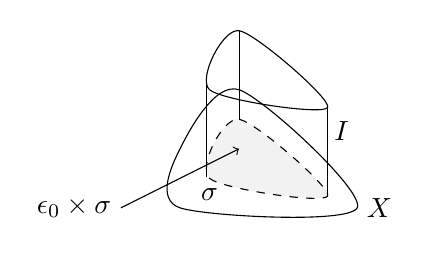
\begin{tikzpicture}[scale = 0.75]
      \draw[] plot [smooth cycle] coordinates {(2,3) (3,4) (5,2) (2,2)};
      \fill[gray!10] plot [smooth cycle] coordinates {(2.5,2.5) (3,3.5) (4.5,2.2)};
      \draw[->] (1,2) -- (3,3);
      \node[left] () at (1,2) {$ \epsilon_0 \times \sigma $};
      \draw[dashed] plot [smooth cycle] coordinates {(2.5,2.5) (3,3.5) (4.5,2.2)};
      \draw[] plot [smooth cycle] coordinates {(2.5,4) (3,5) (4.5,3.7)};
      \draw
      (3,3.5) -- (3,5)
      (4.5,2.2) -- (4.5,3.7)
      (2.45,2.52) -- (2.45,4.1);
      \node[right] () at (5,2) {$ X $};
      \node[below] () at (2.5,2.5) {$ \sigma $};
      \node[right] () at (4.45,3.3) {$ I $};
    \end{tikzpicture}
    \caption{Prisma}
    \label{fig:lez14:prism}
  \end{figure}
  \[
    = \epsilon_1 \times \sigma - \epsilon_0 \times \sigma - I \times \partial \sigma
  \]
  Questa costruzione geometrica corrisponde all'azione dell'operatore prisma:
  \begin{definition}
    Si definisce l'\textbf{operatore prisma}\index{Operatore prisma} definendo
    la sua azione sui simplessi singolari e poi estendendo per linearità:
    \begin{align*}
      D \colon S_q(X) & \to S_{q+1}(X) \\
      \sigma & \mapsto I \times \sigma
    \end{align*}
  \end{definition}
  L'operatore prisma è un omomorfismo in quanto è definito per linearità. La sua
  azione è quella di prendere un simplesso e restituire il prisma in figura.
  % Per  quanto detto sopra vale che:
  Quindi:
  \[
    \partial \circ D (\sigma) + D \circ \partial (\sigma) = \partial (I \times \sigma) + I \times \partial \sigma = (\epsilon_1 \times \sigma - \epsilon_0 \times \sigma - \cancel{I \times \partial \sigma})
    + \cancel{I \times \partial \sigma}
  \]
  Cioè:
  \[
    \partial \circ D (\sigma) + D \circ \partial (\sigma) = \epsilon_1 \times \sigma - \epsilon_0 \times \sigma
  \]
  Nella figura questo sono la faccia superiore e inferiore del prisma.
  Si definiscono le sezioni del prisma, con $ t \in I $:
  \begin{align*}
    \eta_t  \colon X & \to I \times X \\
    x & \mapsto (t,x)
  \end{align*}
  Le sezioni a $ t = 0 $ e a $ t = 1 $ (punti indicati successivamente con
  l'indice $ i \in \set{0,1} $) inducono una mappa sulle catene:
  \begin{align*}
    (\eta_i)_\sharp \colon S_k(X) & \to S_k(I \times X) \\
    \sigma & \mapsto \eta_i \circ \sigma
  \end{align*}
  Ma $ (\eta_i \circ \sigma)(x) = (i, \sigma(x)) = \epsilon_i \times \sigma $, quindi
  $ \partial \circ D (\sigma) + D \circ \partial (\sigma) = (\eta_1)_\sharp(\sigma) - (\eta_0)_\sharp(\sigma) $.

  Per ipotesi $ f_0 $ e $ f_1 $ sono omotopicamente equivalenti quindi esiste
  una funzione continua $ F \colon I \times X \to Y $ tale che:
  \begin{itemize}
  \item $ \forall x \in X $ risulti che $ F(0,x) = f_0(x) $
  \item $ \forall x \in X $ risulti che $ F(1,x) = f_1(x) $
  \item $ \forall t \in I, \forall a \in A $ risulti che  $ F(t,a) \in B $
  \end{itemize}
  Considero la relazione di omotopia $ F \colon I \times X \to Y $, per definizione vale che
  $ F(i,x) = f_i(x) $, e quindi $ (F \circ \eta_i)(x) = f_i(x) $, cioè
  $ F \circ \eta_i = f_i $. Essendo una funzione continua $ F $ induce una mappa sulle
  catene di simplessi: $ F_\sharp \colon S_k(I \times X, I \times A) \to S_k(Y,B) $.

  Considero $ D \colon S_q(X,A) \to S_{q+1}(I \times X, I \times A) $, posso definire
  $ G = F_\sharp \circ D $, questo è un omomorfismo tra $ S_k(X,A) $ e
  $ S_{k+1}(Y,B) $ in quanto composizione di omomorfismi.
  Sia $ c \in S_q(X,A) $ allora:
  \begin{gather*}
    \partial \circ G (c) = \partial (F_\sharp \circ D)(c) \\
    G \circ \partial (c) = (F_\sharp \circ D)(\partial c)
  \end{gather*}
  $ F_\sharp $ è un'applicazione tra complessi e si verifica che una chain map, cioè
  i quadrati che determina sono commutativi ($ F_\sharp \circ \partial = \partial \circ F_\sharp $). In questo modo
  \begin{gather*}
    \partial (F_\sharp \circ D)(c) + (F_\sharp \circ D)(\partial c) = F_\sharp \circ \partial \circ D (c) + F_\sharp \circ D \circ \partial (c) = \\
    = F_\sharp \circ ( \partial \circ D (c) + D \circ \partial (c)) = F_\sharp \circ ( (\eta_1)_\sharp - (\eta_0)_\sharp) (c)
  \end{gather*}
  Quindi $ \partial \circ G + G \circ \partial = (f_1)_\sharp - (f_0)_\sharp $.
  Passando a livello di omologia considero $ k $ un $ q $-ciclo in $ (X,A) $, quindi
  tale che $ \partial k = 0 $. Allora per la definizione di $ f_\sharp $:
  \[
    (f_1)_\star(\llbracket k \rrbracket) = \llbracket(f_1)_\sharp(k)\rrbracket
  \]
  Ma:
  \[
    (f_1)_\sharp(k) = (f_0)_\sharp (k) + \partial \circ G (k) + \cancel{G \circ \partial (k)}
  \]
  Quindi in $ (Y,B) $ vale che
  $ \llbracket(f_1)_\sharp(k)\rrbracket = \llbracket(f_0)_\sharp(k)\rrbracket $ in quanto differiscono per il bordo
  $ \partial(G(k)) $. Quindi
  $ (f_1)_\star(\llbracket k \rrbracket) = (f_2)_\star(\llbracket k \rrbracket) $, ma siccome questo è vero per ogni
  $ k $ allora le mappe devono coincidere, cioè $ (f_1)_\star = (f_2)_\star $.
\end{proof}
\eproof
La mappa $ G $ è un esempio di omotopia di catena:
\begin{definition}
  Siano $ (A_\bullet, \partial^A) $ e $ (B_\bullet, \partial^B) $ complessi, e siano $ \phi, \psi \colon A_\bullet \to B_\bullet $
  mappe continue tra complessi, $ \phi $ e $ \psi $ si dicono \textbf{omotope}\index{Omotopia di catena}
  (\emph{chain homotopic}) se esiste una mappa tra complessi $ D \colon A_\bullet \to B_{\bullet + 1} $
  tale che $ \partial \circ D + D \circ \partial = \phi - \psi $. Si ha quindi il diagramma:
  \[
    \begin{tikzcd}
      \dots \rar & A_{i+1} \rar{\partial^A} & A_i \rar{\partial^A} \arrow{dl}{D} \dar{\phi,\psi} & A_{i-1} \rar \arrow{dl}{D}  & \dots \\
      \dots \rar & B_{i+1} \rar{\partial^B} & B_i \rar{\partial^B} & B_{i-1} \rar & \dots
    \end{tikzcd}
  \]
  Schematicamente:
  \begin{figure}[h]
    \centering
    \begin{tikzpicture}[scale = 0.50]
      \draw
      (0,0) -- (-2,-2)
      (-2,-2) -- (0,-2);
      \draw[-Latex] (0,0) -- (-1,-1);
      \draw[-Latex] (-2,-2) -- (-1,-2);
      \node () at (1,-1) {+};
      \draw
      (3,0) -- (5,0)
      (5,0) -- (3,-2);
      \draw[-Latex] (3,0) -- (4,0);
      \draw[-Latex] (5,0) -- (4,-1);
      \node () at (6,-1) {=};
      \draw
      (7,0) -- (7,-2)
      (9,0) -- (9,-2);
      \draw[-Latex] (7,0) -- (7,-1);
      \draw[-Latex] (9,0) -- (9,-1);
      \node () at (8,-1) {-};
    \end{tikzpicture}
  \end{figure}
\end{definition}
Mappe tra complessi omotope danno origine alla medesima applicazione a livello
di omologia.

\subsection{Omologia ridotta per una qualsiasi teoria omologica}

Sia $ X \not = \emptyset $ spazio topologico e $ p \in X $ punto
($ P = \set{p} $), allora sono ben definite le applicazioni di inclusione $ i $
e la mappa costante $ \epsilon $:
\begin{gather*}
  i \colon P \to X \\
  \epsilon \colon X \to P
\end{gather*}
Si ha che $ \epsilon \circ i = \Id{P} $ in quanto
$ P \overset{i}{\to} X \overset{\epsilon}{\to} P $. Dagli assiomi deriva l'esistenza di
un'applicazione indotta sui gruppi di omologia:
$ \epsilon_\star \colon H_0(X) \to H_0(P) $, questa è suriettiva perché per le proprietà
funtoriali $ (\epsilon \circ i)_\star = (\Id{p})_\star = \Id{H_0(p)} $ e
$ (\epsilon \circ i)_\star = \epsilon_\star \circ i_\star $ quindi $ \epsilon_\star \circ i_\star = \Id{H_0(p)} $, quindi:
\[
  \forall y \in H_0(P) \text{ vale che } (\epsilon_\star \circ i_\star)(y) = y \text{ quindi } \epsilon_\star (i_\star(y)) = y
\]
Sia $ i_\star(y) = x \in H_0(X) $ allora $ \epsilon_\star(x) = y $, quindi $ \epsilon_\star $ è suriettiva.
A partire da ciò posso costruire una successione esatta, infatti per ora ho:
\[
  \begin{tikzcd}
    H_0(X) \rar{\epsilon_\star} & H_0(P) \rar & 0
  \end{tikzcd}
\]
Per il teorema fondamentale degli omomorfismi:
\[
  \quot{H_0(X)}{\ker{\epsilon_\star}} \cong \im{\epsilon_\star} = H_0(P)
\]
Se ora considero la mappa iniettiva
$ \alpha \colon \ker{\epsilon_\star} \incl H_0(X) $, quindi tale che
$ \im{\alpha} = \ker{\epsilon_\star} $, la successione corta è automaticamente esatta (infatti
$ \epsilon_\star \circ \alpha = 0 $, dato che in $ H_0(P) $ il gruppo
$ \ker{\epsilon_\star} $ è ridotto al solo $ 0 $ essendo al quoziente):
\[
  \begin{tikzcd}
    0 \arrow{r}{} & \ker{\epsilon_\star} \arrow{r}{\alpha} & H_0(X) \arrow{r}{\epsilon_\star} & \arrow[bend left]{l}{i_\star} H_0(P) \arrow{r}{} & 0
  \end{tikzcd}
\]
% c'è $ i_\star \colon H_0(P) \to H_0(X) $:
% C'è la successione esatta:
% \[
%   \begin{tikzcd}
%     0 \arrow{r}{} & \ker{\epsilon_\star} \arrow{r}{} & H_0(X) \arrow{r}{\epsilon_\star} & \arrow[bend left]{l}{i_\star} H_0(P) \arrow{r}{} & 0
%   \end{tikzcd}
% \]
Inoltre, siccome $ \epsilon_\star \circ i_\star = \Id{H_0(p)} $, la successione spezza perché
esiste una sezione $ i_\star $, perciò
$ H_0(X) \cong \ker{\epsilon_\star} \oplus H_0(P) $. Questo spezzamento non è naturale e dipende
dalla scelta dell'inclusione $ i $.

Si ha quindi che per qualsiasi teoria omologia che soddisfa gli assiomi di
Eilenberg e Steenrod (infatti ho utilizzato solo gli assiomi), e quindi in
particolare per l'omologia singolare relativa, si ha che
$ H_0(X) \cong \ker{\epsilon_\star} \oplus H_0(P) $.

\newmathsymb{coefgrup}{\mathcal{G}}{Gruppo dei coefficienti}
Generalmente si chiama $ H_0(P) $ il \textbf{gruppo dei coefficienti}\index{Gruppo dei coefficienti di una teoria omologica}
di una teoria omologica e viene denotato con $ \mathcal{G} $. Nell'omologia singolare relativa questo è $ \Z $.
Inoltre si definisce $ \ker{\epsilon_\star} = \tilde{H}_0(X) $ \textbf{gruppo di omologia ridotta di ordine zero}, quindi
ho trovato che $ H_0(X) \cong \tilde{H}_0(X) \oplus \mathcal{G} $.

Cosa sono invece gli $ \tilde{H}_k(X) $? Vorrei che fossero proprio $ H_k(X) $,
così come nel caso dell'omologia singolare.

\begin{proposition}
  In qualsiasi teoria omologica di Eilenberg e Steenrod in cui si definiscono i
  gruppi di omologia ridotta come $ \tilde{H}_k(X) = \ker{\epsilon_X} $ dove
  $ \epsilon_X \colon X \to P $ con $ X $ spazio topologico e $ P = \set{p \in X} $ si ha che:
  \[
    H_k(X) \cong
    \begin{cases}
      \tilde{H}_0(X) \oplus \mathcal{G} & \text{se } k = 0 \\
      \tilde{H}_k(X) & \text{se } k \not= 0
    \end{cases}
  \]
\end{proposition}
\begin{proof}
  % Considero $ F \colon (X, A) \to (P,P) $ con:
  % \[
  %   F =
  %   \begin{cases}
  %     \epsilon_X \colon X \to P \\
  %     \epsilon_A \colon A \to P
  %   \end{cases}
  % \]
  % In generale:
  % \[
  %   \begin{tikzcd}
  %     0 \arrow{r}{}        & \ker{\epsilon_X} \arrow{r}{} & H_k(X) \arrow{r}{\epsilon_\star} & H_k(P) \arrow{r}{}    & 0
  %   \end{tikzcd}
  % \]
  % Per $ k \geq 1 $ $ \ker{\epsilon_X} = H_k(X) $, in quanto per gli assiomi $ H_k(P) \cong 0 $ se $ k \geq 1 $, quindi
  % la successione si riduce a:
  % \[
  %   \begin{tikzcd}
  %     0 \rar & \ker{\epsilon_X} \rar & H_k(X) \rar & 0
  %   \end{tikzcd}
  % \]
  % Mentre per $ k = 0 $ ho che $ H_0(X) \cong \tilde{H}_0(X) \oplus \mathcal{G} $,
  Considero la successione esatta corta:
  \[
    \begin{tikzcd}
      0 \rar & \tilde{H}_k(X) := \ker{\epsilon_X} \rar & H_k(X) \rar & H_k(P) \rar & 0
    \end{tikzcd}
  \]
  Questa spezza in quanto $ \epsilon_X \colon X \to P $ ammette un'inversa
  $ i_X \colon P \to X $ e quindi a livello di omologia esiste
  $ (i_X)_\star \colon H_k(P) \to H_k(X) $ inversa di
  $ (\epsilon_X)_\star \colon H_k(X) \to H_k(P) $. Ma per gli assiomi i gruppi
  di omologia di un punto sono banali per $ k > 0 $, mentre
  per $ k = 0 $ si pone $ H_0(P) = \mathcal{G} $ con $ \mathcal{G} $ gruppo dei coefficienti.
  Quindi siccome $ H_k(X) = \tilde{H}_k(X) \oplus G $:
  \[
    \tilde{H}_k(X) =
    \begin{cases}
      H_k(X)               & \text{per } k \geq 1 \\
      \tilde{H}_0(X) \oplus \mathcal{G} & \text{per } k = 0 \\
    \end{cases}
  \]
  Sostanzialmente l'omologia ridotta elimina dallo $ 0 $-esimo
  gruppo di omologia un fattore $ \mathcal{G} $.
  % \[
  %   \begin{tikzcd}[nodes={column sep=10pt, row sep=5pt}]
  %      {} & {} & 0  \arrow{dr}{} & {} & {}  & 0 \arrow{dr}{} & {} & {}  & {}    \\
  %      0 \rar & H_1(P,P) \arrow{rr}{}  \arrow{ur}{}  & {}  & H_{0}(P) \rar &  H_{0}(P) \arrow{rr}{}  \arrow{ur}{}
  %     & {} & H_{0}(P,P) \rar & 0
  %   \end{tikzcd}
  % \]
  % E quindi $ H_1(P,P) = 0 $ e $ H_0(P,P) = 0 $.
\end{proof}
\eproof
Questo lo posso fare anche nel caso di una coppia se $ A $ è sottospazio
  topologico di $ X $ definendo $ F \colon (X, A) \to (P,P) $ con:
  \[
    F =
    \begin{cases}
      \epsilon_X \colon X \to P \\
      \epsilon_A \colon A \to P
    \end{cases}
  \]
  Si ha la successione esatta corta:
  \[
    \begin{tikzcd}
      0 \arrow{r}{}        & \ker{F_\star} \arrow{r}{} & H_k(X, A) \arrow{r}{} & H_k(P, P) \arrow{r}{} & 0
    \end{tikzcd}
  \]
  E si definisce $ \tilde{H}_k(X,A) = \ker{F_\star} $.
  % Calcolo $ H_k(P,P) $ con $ P $ spazio formato da un solo punto in $ X $.
  Gli assiomi richiedono l'esistenza di una successione esatta lunga per coppie $ (X,A) $,
  ponendo $ X = A = P $ si ottiene:
  \[
    \begin{tikzcd}
      \dots \arrow{r}{}        & H_k(P) \arrow{r}{}    & H_k(P) \arrow{r}{}    & H_k(P,P) \arrow{r}{}  & H_{k-1}(P) \arrow{r}{} & \dots
    \end{tikzcd}
  \]
  % Cioè ho posto $ X = P $ e $ A = P $.
  Sempre gli assiomi richiedono che l'omologia di un punto sia nulla per
  $ k \geq 1 $ mentre valga il gruppo dei coefficienti per $ k = 0 $. Supponendo
  $ k \geq 2 $ la successione diventa:
  \[
    \begin{tikzcd}
       0 \arrow{r}{} & H_k(P,P) \arrow{r}{}  & 0
    \end{tikzcd}
  \]
  E quindi $ H_k(P, P) = 0 $. Mentre se $ k = 1 $ allora:
  \[
    \begin{tikzcd}[nodes={column sep=10pt}]
      \dots \arrow{r}{}        & H_1(P) \arrow{r}{}    & H_1(P) \arrow{r}{}    & H_1(P,P) \arrow{r}{}  & H_{0}(P) \arrow{r}{}   &
      H_{0}(P) \arrow{r}{} & H_{0}(P,P) \rar       & 0
    \end{tikzcd}
  \]
  Cioè siccome $ H_1(P) \cong 0 $:
  \[
    \begin{tikzcd}
       0 \arrow{r}{}         & H_1(P,P) \arrow{r}{i}  & H_{0}(P) \arrow{r}{j}   & H_{0}(P) \arrow{r}{k} & H_{0}(P,P) \rar       & 0
    \end{tikzcd}
  \]
  Ma quindi ho $ H_0(P) \to H_0(P) $ che sarebbe $ H_0(A) \to H_0(X) $ e quindi la
  mappa che li collega è quella indotta dall'inclusione, che per $ X = A = P $ e
  l'identità, ma per la funtorialità viene mandata nell'identità, quindi $ j $ è
  isomorfismo. Per l'esattezza della successione $ \im{i} = \ker{j} = 0 $ in
  quanto $ j $ è iniettiva, e quindi posso riscrivere la prima parte della
  successione come:
  \[
    \begin{tikzcd}
      0 \rar & H_1(P,P) \rar & 0
    \end{tikzcd}
  \]
  Da cui $ H_1(P,P) = 0 $. Similmente $ \ker{k} = \im{j} = H_0(P) $ quindi $ H_0(P,P) = 0 $ perché
  $ H_0(P,P) \cong {H_0(P)} \slash {\ker{k}} \cong {H_0(P)} \slash {H_0(P)} = 0 $.
  Avendo trovato che $ \forall k $ $ H_k(P,P) = 0 $ allora si ha che $ \ker{F_\star} \cong H_k(X,A) $.

\begin{corollary}
  Se $ X $ è uno spazio topologico contraibile allora $ \tilde{H}_k(X) = 0 $.
\end{corollary}
\begin{proof}
  Se $ X $ è contraibile allora $ X \sim_H P $ cioè $ \exists f \colon X \to P $ e $ \exists g \colon P \to X $
  continue tali che $ f \circ g \sim_H \Id{P} $ e $ g \circ f \sim_H \Id{X} $, quindi
  per la funtorialità e l'assioma dell'omotopia vale che passando a livello
  di omologia:
  $ f_\star \circ g_\star = \Id{H_k(P)} $ e  $ g_\star \circ f_\star = \Id{H_k(X)} $
  % con $ f_\star \colon H_k(X) \to H_k(P) $  e  $ g_\star \colon H_k(P) \to H_k(X) $,
  quindi $ f_\star $ e $ g_\star $ sono inversi l'una dell'altra, ma sempre per la funtorialità:
  $ (f \circ g)_\star = \left( \Id{P} \right)_\star $ e $ (g \circ f)_\star = \left( \Id{X} \right)_\star $,
  quindi $ f_\star $ e $ g_\star $ realizzano un isomorfismo tra i gruppi di omologia:
  \[
   H_k(X) \cong H_k(P) \cong
    \begin{cases}
      0 & \text{se } k \geq 1 \\
      \mathcal{G} & \text{se } k = 0
    \end{cases}
  \]
  Quindi $ \tilde{H}_k(X) = 0 $ per $ k \geq 1 $ e per $ k = 0 $ vale che
  $ \mathcal{G} = H_0(P) = \tilde{H}_0(X) \oplus \mathcal{G} $ e quindi
  $ \tilde{H}_0(X) = 0 $.
\end{proof}
\begin{corollary}
  La sfera la non è contraibile, infatti come si vedrà a breve i suoi gruppi di
  omologia ridotta non sono sempre banali.
\end{corollary}

\newmathsymb{spheres}{\Sph{n}}{$ n $-sfera}
\newmathsymb{disks}{\Disk{n}}{$ n $-disco}
\newmathsymb{updisk}{\Disk{n}_+}{Calotta superiore dell'$ n $-disco}
\section{Omologia delle sfere}
\begin{theorem}[Omologia di dischi e sfere]
  Siano per $ n \geq 1$:
  \begin{gather*}
    \Sph{n} = \set{\vec{x} \in \RN{n+1} | ||\vec{x}||^2 = 1} \\
    \Disk{n} = \set{\vec{x} \in \RN{n} | ||\vec{x}||^2 \leq 1} \\
    \Disk{n}_+ = \set{\vec{x} \in \RN{n} | ||\vec{x}||^2 \leq 1, x_n \geq 0}
  \end{gather*}
  Allora in una qualsiasi teoria omologica avente $ \mathcal{G} $ come
  gruppo dei coefficienti:
  \begin{align*}
    \tilde{H}_k(\Sph{n}) & \cong
    \begin{cases}
      \mathcal{G} & \text{se } k = n \\
      0 & \text{se } k \not = n
    \end{cases} \\
    H_k(\Disk{n}, \Sph{n-1}) & \cong
    \begin{cases}
      \mathcal{G} & \text{se } k = n \\
      0 & \text{se } k \not = n
    \end{cases} \\
    H_k(\Sph{n}, \Disk{n}_+) & \cong
    \begin{cases}
      \mathcal{G} & \text{se } k = n \\
      0 & \text{se } k \not = n
    \end{cases}
  \end{align*}
  Quindi $ \tilde{H}_k(\Sph{n}) \cong H_k(\Disk{n}, \Sph{n-1}) \cong H_k(\Sph{n}, \Disk{n}_+) $.
\end{theorem}
\begin{proof}
  La dimostrazione è per passi:
  \begin{enumerate}
  \item Dimostro che
    \[
      H_k(\Sph{0}, \Disk{0}_+) = H_k(\Sph{0}, \Disk{0}) \cong
      \begin{cases}
        \mathcal{G} & \text{se $ k = 0 $} \\
        0 & \text{se $ k \not = 0 $}
      \end{cases}
    \]
  \item Mostro che $ H_k(\Sph{n}, \Disk{n}) \cong \tilde{H}_k(\Sph{n}) $
  \item Mostro che $ H_k(\Disk{n}, \Sph{n-1}) \cong \tilde{H}_k(\Sph{n}, \Disk{n}) $
  \item Mostro che $ H_k(\Disk{n}, \Sph{n-1}) \cong \tilde{H}_{k-1}(\Sph{n01}) $
  \item A partire dai punti precedenti calcolo tutti i gruppi di omologia
  \end{enumerate}

  \subparagraph{Dimostrazione del punto uno}
  % Comincio calcolando $ H_k(\Sph{0}, \Disk{0}_+) $.
  Si ha che $ \Sph{0} = \set{-1, +1} $ e $ \Disk{0} = \Disk{0}_+ = \set{+ 1} $.
  Siccome $ \Disk{0} \subseteq \Sph{0} $ per l'assioma dell'esattezza esiste
  una successione esatta in omologia:
  \[
    \begin{tikzcd}
      \dots \rar & H_k(\Disk{0}) \rar & H_k(\Sph{0}) \rar & H_k(\Sph{0}, \Disk{0}) \rar & H_{k-1}(\Disk{0}) \rar & \dots
    \end{tikzcd}
  \]
  Per $ k \geq 2 $ $ H_k(\Disk{0}) = H_{k-1}(\Disk{0}) \cong 0 $ perché $ \Disk{0} $ è un punto, quindi
  la successione diventa:
  \[
    \begin{tikzcd}
      0 \rar & H_k(\Sph{0}) \rar{i} & H_k(\Sph{0}, \Disk{0}) \rar{} & 0
    \end{tikzcd}
  \]
  Ma per l'assioma di additività, siccome $ \Sph{0} $ è la somma di due punti
  $ H_k(\Sph{0}) \cong 0 $, essendo la successione esatta
  % siccome $ i $ è iniettiva perché la successione è esatta
  % ed è suriettiva perché essendo la successione esatta $ \im{i} = \ker{j} =  H_k(\Sph{0}, \Disk{0}) $
  $ i $ è isomorfismo quindi anche $ H_k(\Sph{0}, \Disk{0}) \cong 0 $.
  Per calcolare
  i casi $ k = 1 $ e $ k = 0 $ considero la successione esatta:
  \[
    \begin{tikzcd}[nodes={column sep=10pt, inner sep=4pt}]
      \dots \rar & H_1(\Disk{0}) \rar & H_1(\Sph{0}) \rar & H_1(\Sph{0}, \Disk{0}) \rar
      & H_0(\Disk{0}) \rar & H_{0}(\Sph{0}) \rar & H_0(\Sph{0}, \Disk{0}) \rar & 0
    \end{tikzcd}
  \]
  Cioè siccome l'omologia di un punto è nulla per $ k \not = 0 $:
  \[
    \begin{tikzcd}
       0 \rar & H_1(\Disk{0}, \Sph{0}) \rar{i}
      & H_0(\Disk{0}) \rar{j} & H_{0}(\Sph{0}) \rar & H_0(\Sph{0}, \Disk{0}) \rar & 0
    \end{tikzcd}
  \]
  Siccome $ \Disk{0} \incl \Sph{0} $ in quanto $ \set{+1} \incl \set{-1, +1} $ è
  inieittiva a livello di omologia per l'assioma di additività
  $ j \colon H_0(\set{+1}) \to H_0(\set{-1}) \oplus H_0(\set{+1}) $ è iniettiva, quindi
  $ \ker{j} = \im{i} = 0 $, ma $ i $ è iniettiva quindi manda solo lo zero
  in zero e perciò $ H_1(\Sph{0},\Disk{0}) \cong 0 $.
  % quindi posso riscrivere la prima  parte della successione come:
  % \[
  %   \begin{tikzcd}
  %     0 \rar & H_1(\Sph{0},\Disk{0}) \rar & 0
  %   \end{tikzcd}
  % \]
  % Da cui $ H_1(\Sph{0},\Disk{0}) = 0 $ per lo stesso ragionamento di prima.
  Infine per definizione $ H_0(\Disk{0}) = \mathcal{G} $ e
  per l'assioma di additività $ H_0(\Sph{0}) = \mathcal{G} \oplus \mathcal{G} $ quindi
  $ H_0(\Sph{0}, \Disk{0}) \cong {\mathcal{G} \oplus \mathcal{G}} \slash {\mathcal{G}} \cong \mathcal{G} $.
  In conclusione:
  \[
    H_k(\Sph{0}, \Disk{0}) \cong
    \begin{cases}
      \mathcal{G} & \text{se } k = 0 \\
      0 & \text{se } k \not =  0
    \end{cases}
  \]

  \subparagraph{Dimostrazione del punto due}
  % Mi rimane da verificare l'ultimo, osservo intanto che $ \Disk{n}_+ \simeq \Disk{n} $,
  % quindi in quello che segue sostanzialmente ometto il $ + $.

  Considero la successione esatta indotta dall'inclusione $ \Disk{n} \incl \Sph{n} $:
  \[
    \begin{tikzcd}
      \dots \rar & H_k(\Disk{n}) \rar & H_k(\Sph{n}) \rar & H_k(\Sph{n}, \Disk{n}) \rar & H_{k-1}(\Disk{n}) \rar & \dots
    \end{tikzcd}
  \]
  Per $ k \geq 2 $ ho che $ H_k(\Disk{n}) \cong 0 $ e che $ H_{k-1}(\Disk{n}) \cong 0 $ quindi
  la successione diventa:
  \[
    \begin{tikzcd}
      0 \rar & H_k(\Sph{n}) \rar & H_k(\Sph{n}, \Disk{n}) \rar & 0
    \end{tikzcd}
  \]
  Quindi
  $ H_k(\Sph{n}, \Disk{n}) \cong H_k(\Sph{n}) \cong \tilde{H}_k(\Sph{n}) $ per
  $ k \geq 2 $. Per $ k = 1 $ e $ n \not = 1 $ la successione è:
  \[
    \begin{tikzcd}[nodes={column sep=10pt}]
      0 \rar & H_1(\Sph{n}) \rar & H_1(\Sph{n}, \Disk{n}) \rar & H_0(\Disk{n}) \rar & H_0(\Sph{n}) \rar & H_0(\Sph{n}, \Disk{n}) \rar & 0
    \end{tikzcd}
  \]
  Ma $ H_0(X) $ conta le componenti connesse per archi di $ X $ quindi
  $ H_0(\Disk{n}) \cong H_0(\Sph{n}) $ e quindi per lo stesso motivo di prima
  $ H_1(\Sph{n}, \Disk{n}) \cong H_0(\Sph{n}, \Disk{n}) \cong 0 $
  \[
    H_k(\Sph{n}, \Disk{n}) \cong
    \begin{cases}
      \tilde{H}_k(\Sph{n}) & \text{se } k \geq 2 \\
      0 & \text{se } k \in \set{0,1}
    \end{cases}
  \]
  Se $ n \geq 2 $ allora $ \tilde{H}_k(\Sph{n}) = 0 $ per $ k \in \set{0,1} $
  $ \Sph{n} $ sono semplicemente connesse quindi
  $ \tilde{H}_1(\Sph{n}) = H_1(\Sph{n}) = 0 $, e c'è una sola componente
  connessa per archi quindi $ H_0(\Sph{n}) = 0 $ e perciò
  $ H_k(\Sph{n}, \Disk{n}) \cong \tilde{H}_k(\Sph{n}) $. Nel caso $ n = 1 $ vale che
  $ H_1(\Sph{1}, \Disk{1}) = \mathcal{G} $ ma anche
  $ \tilde{H}_1(\Sph{1}) = \mathcal{G} $ e quindi anche in questo caso
  $ H_k(\Sph{n}, \Disk{n}) \cong \tilde{H}_k(\Sph{n}) $.

  \subparagraph{Dimostrazione del  punto tre}
  Considero $ U $ intorno chiuso del polo nord di $ \Sph{n} $,
  per il teorema di escissione:
  \[
    H_p(\Sph{n}, \Disk{n}) \cong H_p(\Sph{n} \setminus U, \Disk{n} \setminus U )
  \]
  Per l'equivalenza omotopica
  $ H_p(\Sph{n} \setminus U, \Disk{n} \setminus U ) \cong H_p(\Disk{n}, \Sph{n-1}) $, infatti
  \[
    \Sph{n} \setminus U \sim_H \Disk{n} \text{ e } \Disk{n} \setminus U \sim_H \Sph{n-1}
  \]
  In quanto dalla sfera tolgo una calotta intorno al polo Nord e quello che rimane
  è omeomoerfo ad un disco, se dal disco tolgo un dischetto intorno al centro
  quello che rimane è omeomorfo al bordo del disco.

  \subparagraph{Dimostrazione del punto quattro}

  % Mostro che $ \tilde{H}_{k-1}(\Sph{n-1}) \cong H_k(\Disk{n}, \Sph{n-1}) $.
  % \[
  %   \tilde{H}_k(\Sph{n}) \cong
  %   \begin{cases}
  %     \mathcal{G} & \text{se } k = n \\
  %     0 & \text{se } k \not = n
  %   \end{cases}
  % \]
  Ho che $ \Sph{n-1} $ è il bordo di $ \Disk{n} $ quindi c'è una mappa naturale di inclusione
  ed è ben definita la successione esatta lunga:
  \[
    \begin{tikzcd}[nodes={column sep=4.5pt, inner sep=0.5pt}]
      \dots \rar & H_k(\Sph{n-1}) \rar & H_k(\Disk{n}) \rar & H_k(\Disk{n}, \Sph{n-1}) \rar
      & H_{k-1}(\Sph{n-1}) \rar & H_{k-1}(\Disk{n}) \rar & H_{k-1}(\Disk{n}, \Sph{n-1}) \rar & \dots
    \end{tikzcd}
  \]
  Per $ k \geq 1 $ $ H_k(\Disk{n}) = 0 $ perché $ \Disk{n} $ è contraibile, quindi ho la successione:
  \[
    \begin{tikzcd}[nodes={column sep=10pt}]
      0 \rar & H_k(\Disk{n}, \Sph{n-1}) \rar & H_{k-1}(\Sph{n-1}) \rar & H_{k-1}(\Disk{n}) \rar & H_{k-1}(\Disk{n}, \Sph{n-1}) \rar & \dots
    \end{tikzcd}
  \]
  Se $ k \geq 2 $ la successione si riduce a:
  \[
    \begin{tikzcd}[nodes={column sep=10pt}]
      0 \rar & H_k(\Disk{n}, \Sph{n-1}) \rar{i} & H_{k-1}(\Sph{n-1}) \rar & 0
    \end{tikzcd}
  \]
  Quindi $ i $ è inieittiva e suriettiva e perciò
  $ H_k(\Disk{n}, \Sph{n-1}) \cong H_{k-1}(\Sph{n-1}) \cong \tilde{H}_{k-1}(\Sph{n-1}) $.
  Per $ k = 1 $ ho la successione:
  \[
    \begin{tikzcd}[nodes={column sep=10pt}]
      0 \rar & H_1(\Disk{n}, \Sph{n-1}) \rar & H_0(\Sph{n-1}) \rar & H_0(\Disk{n}) \rar & H_0(\Disk{n}, \Sph{n-1}) \rar & 0
    \end{tikzcd}
  \]
  Utilizzando  le stesse argomentazioni del punto precedente si trova che
  $ \forall k \geq 0 \text{ e } \forall n > 0 $ $ H_k(\Disk{n}, \Sph{n-1}) = \tilde{H}_{k-1}(\Sph{n-1}) $ .
  % Quindi $ H_1(\Disk{n}, \Sph{n-1}) = 0 $ per i soliti motivi.
  % Ma esiste $ i \colon \Sph{n-1} \incl \Disk{n} $ iniettiva, quindi esiste $ i_\star \colon H_0(\Sph{n-1}) \to H_0(\Disk{n}) $.
  % Ma $ \Disk{n} $ è contraibile quindi posso prendere come generatore un punto di $ \Disk{n} $, e ne prendo
  % uno sul bordo, cioè in $ \Sph{n-1} $, quindi:
  % \begin{align*}
  %   i_\star \colon H_0(\Sph{n-1}) & \to H_0(\Disk{n}) \\
  %   \llbracket p \rrbracket & \mapsto \llbracket p \rrbracket
  % \end{align*}
  % Quindi $ H_0(\Disk{n}, \Sph{n-1}) = 0 $ in quanto $ H_0(\Sph{n-1}) \to H_0(\Disk{n}) $ è iniettiva
  % e suriettiva e $ H_0(\Disk{n}, \Sph{n-1}) \cong \quot{H_0(\Disk{n})}{H_0(\Sph{n-1})} \cong 0 $.
  % In conclusione ho trovato che $ H_k(\Disk{n}, \Sph{n-1}) = 0 $ per $ k \in \set{0,1} $.

  % Rimane da vedere come si comportano i gruppi di omologia
  % $ \tilde{H}_k(\Sph{n}) $ con $ k \geq 1 $. Per $ n = 0 $ è noto perché sono
  % $ \Sph{0} $ sono due punti, per $ k = 0 $ anche perché sono connessi per
  % archi, infine so che: $ H_k(\Sph{n}) \cong \tilde{H}_k(\Sph{n}) $ per
  % $ k \geq 1 $, ma anche che $ H_k(\Sph{n}, \Disk{n}) \cong H_k(\Sph{n}) $, se mostro
  % che $ H_p(\Sph{n}, \Disk{n}) \cong H_p(\Disk{n}, \Sph{n-1}) $ allora
  % $ H_k(\Sph{n}, \Disk{n}) \cong H_k(\Disk{n}, \Sph{n-1}) $.

  % Per far vedere che $ H_p(\Sph{n}) \cong H_p(\Disk{n}, \Sph{n-1}) $ uso l'escissione:

  \subparagraph{Dimostrazione del punto cinque}
  % Ma ho mostrato che
  % $ H_k(\Disk{n}, \Sph{n-1}) \cong H_{k-1}(\Sph{n-1}) $, quindi posso procedere per
  % induzione:
  % \[
  %   \tilde{H}_k(\Sph{n}) \cong H_k(\Sph{n}) \cong H_k(\Sph{n}, \Disk{n}) \cong H_k(\Disk{n}, \Sph{n-1}) \cong H_{k-1}(\Sph{n-1}) \cong \dots
  % \]

  Ho mostrato che:
  \[
    \tilde{H}_k(\Sph{n}) \cong H_{k+1}(\Sph{n+1}, \Disk{n+1}) \cong \tilde{H}_{k+1}(\Sph{n+1})
  \]
  Quindi parto da quello che ho calcolato, cioè $ H_k(\Sph{0}, \Disk{0}) $ e salgo:
  $ H_k(\Sph{0}, \Disk{0}) \cong H_{k+n}(\Sph{n}, \Disk{n}) $, quindi:
  \[
    H_{k+n}(\Sph{n}, \Disk{n}) \cong
    \begin{cases}
      \mathcal{G} & \text{se } k = 0 \\
      0 & \text{se } k \not = 0
    \end{cases}
  \]
  Cioè:
  \[
    H_{p}(\Sph{n}, \Disk{n}) \cong
    \begin{cases}
      \mathcal{G} & \text{se } k = n \\
      0 & \text{se } k \not = n
    \end{cases}
  \]
  Quindi gli isomorfismi che ho trovato trovo che:
  \begin{align*}
    \tilde{H}_p(\Sph{n}) & \cong
    \begin{cases}
      \mathcal{G} & \text{se } p = n \\
      0 & \text{se } p \not = n
    \end{cases} \\
    H_p(\Disk{n}, \Sph{n-1}) & \cong
    \begin{cases}
      \mathcal{G} & \text{se } p = n \\
      0 & \text{se } p \not = n
    \end{cases}
  \end{align*}
  E inoltre:
  \[
    H_{p}(\Sph{n}, \Disk{n}_+) \cong
    \begin{cases}
      \mathcal{G} & \text{se } p = n \\
      0 & \text{se } p \not = n
    \end{cases}
  \]
  Dove si è usato che $ \Disk{n}_+ \simeq \Disk{n} $.
\end{proof}

% lezione 7

%  _      _____ ________ ___  _   _ _____   _____
% |  |   | ____|__  /_ _/ _ \| \ | | ____| |___  |
% |  |   |  _|   / / | | | | |  \| |  _|      / /
% |  |___| |___ / /_ | | |_| | |\  | |___    / /
% | _____|_____/____|___\___/|_| \_|_____|  /_/
\begin{corollary}
  Se il gruppo dei coefficienti è $ \Z $:
  \[
    H_k(\Sph{n}) \cong
    \begin{cases}
      \Z & \text{se } k \in \set{0, n} \\
      0 & \text{se } k \not \in \set{0, n}
    \end{cases}
  \]
\end{corollary}
Questo risultato ha numerose conseguenze, infatti ho trovato uno
strumento più fine del gruppo fondamentale che riesce a distinguere
spazi diversi.

\begin{corollary}
  $ \Sph{n} \simeq \Sph{m} $ se e solo se $ n = m $.
\end{corollary}
\begin{proof}
  Se $ n = m $ vale che $ \Sph{n} = \Sph{m} $ quindi in particolare
  $ \Sph{n} \simeq \Sph{m} $ con la mappa identità. Assumo $ n \not = m $ e senza
  perdita di generalità pongo $ n > m $. Per assurdo $ \Sph{n} \simeq \Sph{m} $,
  quindi esiste un omeomorfismo $ F: \Sph{n} \homoto \Sph{m} $, quindi esiste
  anche l'omeomorfismo inverso $ G: \Sph{m} \homoto \Sph{n} $. Quindi esistono
  anche:
  \[
    F_\star: H_k(\Sph{n}) \to H_k(\Sph{m}) \quad \text{e} \quad G_\star: H_k(\Sph{m}) \to H_k(\Sph{n})
  \]
  Ma $ F \circ G = \Id{\Sph{n}} $ e $ G \circ F = \Id{\Sph{m}} $ perché sono omeomorfismi,
  ma utilizzando la funtorialità si trova quindi che:
  \[
    F_\star \circ G_\star = \Id{H_k(\Sph{m})} \quad \text{e} \quad G_\star \circ F_\star = \Id{H_k(\Sph{n})}
  \]
  Da cui si deduce che $ F_\star $ e $ G_\star $ sono continue e sono inverse l'una
  dell'altra.
  Vale quindi che:
  \[
    H_k(\Sph{n}) \cong H_k(\Sph{m}) \; \forall k \geq 0
  \]
  Se vale per ogni $ k $ in particolare vale per $ k = n $, cioè:
  \[
    H_n(\Sph{n}) = H_n(\Sph{m})
  \]
  Ma $ H_n(\Sph{n}) \cong \Z $ e $ H_n(\Sph{m}) \cong 0 $ da cui $ \Z \cong 0 $, che è assurdo.
\end{proof}

\begin{corollary}[Invarianza topologica della dimensione]
  Vale che $ \RN{n} \simeq \RN{m} $ se e solo se $ n = m $.
\end{corollary}
% Come si è visto non si riesce a dimostrare questo corollario
% utilizzano solo il gruppo fondamentale.
% \\ \noindent
\begin{proof}
  Per assurdo esiste un omomorfismo $ f \colon \RN{n} \homoto \RN{m} $ con $ n > m > 2 $.
  Con i vincolo imposti su $ m $ e $ n $ gli spazi sono contraibili, quindi il gruppo
  fondamentale è in entrambi i casi banale. Togliendo un punto $ p \in \RN{n} $ e
  $ f(p) \in \RN{m} $, e restringendo $ f $ in modo da ottenere l'omomorfismo
  $ f' \colon \RN{n} \setminus \set{p} \homoto \RN{m} \setminus \set{f(p)} $.
  Si sa inoltre che per $ s \geq 2 $ vale che $ \RN{s} \setminus \set{q} \simeq \Sph{s-1} \times \RN{} $,
  infatti è sufficiente mandare a $ 0 $ il punto $ q $ con una traslazione
  (che è certamente un omomorfismo) e quindi si ha:
  \begin{align*}
    \RN{k} \setminus \set{q}  \to  \Sph{k-1} \times {\RN{}}^+  \simeq \Sph{k-1} \times \RN{} \\
    \vec{x} \mapsto \left(\frac{\vec{x}}{|| \vec{x} ||}, || \vec{x} || \right)
  \end{align*}
  Quindi:
  \[
    \RN{n} \setminus \set{p} \simeq \RN{m} \setminus \set{f(p)} \iff \Sph{n-1} \times \RN{} \simeq \Sph{m-1} \times \RN{}
  \]
  Si ha la tentazione di eliminare $ \RN{} $ dalla precedente relazione, ma
  questo non si può fare come mostrano alcuni casi molto patologici.
  Tuttavia è possibile passare alla omotopia sapendo che $ \Sph{k} \times \RN{} \sim \Sph{k} $,
  da cui $ \Sph{n-1} \sim \Sph{m-1} $. Ma l'omologia è invariante omotopico, cioè
  $ H_k(\Sph{n-1}) \cong H_k(\Sph{m-1}) $, utilizzando il trucco di prima scelgo $ k = n-1 $
  e quindi:
  \[
    H_{n-1}(\Sph{n-1}) \cong H_{n-1}(\Sph{m-1}) \iff \Z \cong 0
  \]
  Che è assurdo.
\end{proof}
\eproof
Un corollario del precedente risultato richiede la definizione di retratto di deformazione:
\begin{definition}
  Uno spazio topologico $ Y $ si dice \textbf{retratto di deformazione}\index{Retratto di deformazione} di un altro
  spazio topologico $ X $ tale che $ Y \incl X $ se esiste una funzione continua $ r\colon X \to Y $ che inverte a meno di omotopia
  la mappa di inclusione $ i\colon Y \to X $, cioè tale che soddisfa:
  \begin{enumerate}
  \item $ r\colon X \to Y $ continua
  \item $ i \circ r \sim \Id{X} $
  \item $ r \circ i = \Id{Y} $
  \end{enumerate}
  Una mappa che soddisfa queste condizioni è detta \textbf{retrazione}\index{Retrazione}.
\end{definition}
\begin{osservation}
  Se $ Y $ è un retratto di deformazione di $ X $ allora $ X $ e $ Y $ sono
  omotopicamente equivalenti e la mappa di equivalenza omotopica è proprio
  l'inclusione.
\end{osservation}
\begin{corollary}
  $ \Sph{n-1} $ non è un retratto di deformazione di $ \Disk{n} $ per $ n \geq 2 $,
  cioè il disco non è retraibile sul suo bordo.
\end{corollary}
\begin{proof}
  Si ricorda che:
  \[
    \Disk{n} = \set{ \vec{x} \in \RN{n} | || \vec{x} || \leq 1} \quad \Sph{n-1} = \partial \Disk{n} = \set{ \vec{x} \in \RN{n} | || \vec{x} || = 1}
  \]
  Chiaramente esiste $ i \colon \Sph{n-1} \incl \Disk{n} $.
  Suppongo per assurdo che $ \Sph{n-1} $ è un retratto di deformazione di $ \Disk{n} $, cioè che
  esiste una retrazione $ r $. Passando all'omologia:
  \begin{gather*}
    i_\star \colon H_k(\Sph{n-1}) \to H_k(\Disk{n}) \\
    r_\star \colon H_k(\Disk{n}) \to H_k(\Sph{n-1}) \\
    \left( i \circ r \right)_\star = (\Id{\Disk{n}})_\star \text{ e }  \left( r \circ i \right)_\star = (\Id{\Sph{n-1}})_\star
  \end{gather*}
  Quindi per la funtorialità:
  \[
    i_\star \circ r_\star = \Id{H_k(\Disk{n})} \text{ e } r_\star \circ i_\star = \Id{H_k(\Sph{n-1})} \; \forall k \in \mathbb{N}
  \]
  In particolare considero $ k = n - 1 $:
  \begin{gather*}
    i_\star \colon H_{n-1}(\Sph{n-1}) \to H_{n-1}(\Disk{n}) \\
    r_\star \colon H_{n-1}(\Disk{n}) \to H_{n-1}(\Sph{n-1})
  \end{gather*}
  Cioè: $ i_\star \colon \Z \to 0 $. Considero un generatore $ \alpha $ di $ H_{n-1}(\Sph{n-1}) \cong \Z $, cioè tale
  che $ \langle\alpha\rangle = H_{n-1}(\Sph{n-1}) $ allora $ i_\star(\alpha) = 0 $ quindi $ r_\star \circ i_\star = 0 $, ma
  $ \left( r \circ i \right)_\star = \Id{\Sph{n-1}_\star} $ quindi significherebbe $ \Id{\Sph{n-1}_\star}(\alpha) = 0 $,
  cioè che $ \alpha = 0 $, che è assurdo perché $ \Z \not = \langle0\rangle $.
\end{proof}

\begin{theorem}[Punto fisso di Brouwer\index{Teorema del punto fisso}]
  Ogni funzione continua $ g \colon \Disk{n} \to \Disk{n} $ con $ n \geq 2 $ ammette almeno un punto fisso
  in $ \Disk{n} $, cioè:
  \[
    \exists \vec{x_0} \in \Disk{n} \; | \; g(\vec{x_0}) = \vec{x_0}
  \]
\end{theorem}
\begin{proof}
  Per assurdo $ g $ non ammette punto fisso ogni punto $ \vec{x} \in \Disk{n} $ è
  tale che $ g(\vec{x}) \not = \vec{x} $ con  $ g(\vec{x}) \in \Disk{n} $.
  Considero la retta $ l $ passante per $ \vec{x} $ e $ g(\vec{x}) $. Questa retta
  interseca il bordo di $ \Disk{n} $ in due punti $ \set{p_1, p_2} $:
  \[
    l \cap \partial \Disk{n} = l \cap \Sph{n-1} = \set{p_1, p_2}
  \]
  Definisco la mappa $ r \colon \Disk{n} \to \partial \Disk{n} = \Sph{n-1} $ tale che associ
  ad ogni punto del disco il punto di intersezione della retta $ l_{\vec{x}} $ che gli sta più
  vicino (infatti in $ \RN{n} $ è ben definita una nozione di distanza). La retta $ l_{\vec{x}} $
  è ben definita in quanto per due punti distinti (e per ipotesi  $ g(\vec{x}) \not = \vec{x} $)
  passa una e una sola retta.
  \begin{figure}[htbp]
    \centering
    \begin{tikzpicture}
      \draw (0,0) circle (2);
      \draw[-Latex] (-2.5, 0) -- (2.5,0);
      \draw[-Latex] (0, -2.5) -- (0, 2.5);
      \draw (-2, -2.33) -- (2, 3);
      \node[below, right] () at (0.5, 1) {$ g(\vec{x}) $};
      \node[] () at (0.5, 1) {\textbullet};
      \node[above] () at (-1, -1) {$ \vec{x} $};
      \node[] () at (-1, -1) {\textbullet};
      \node[left] () at (2, 3) {$ l $};
      \node[below, left] () at (-1.35, -1.47) {$ p_1 $};
      \node[] () at  (-1.35, -1.47) {\textbullet};
      \node[above, right] () at (1.04, 1.71) {$ p_2 $};
      \node[] () at  (1.04, 1.70) {\textbullet};
    \end{tikzpicture}
    \caption{Schema per $ n = 2 $}
    \label{fig:lez7:brouwer_proof_1}
  \end{figure}
  \begin{exercise}
    Dimostrare che $ r $ è continua.
  \end{exercise}
  Ho una mappa di inclusione naturale:
  \begin{align*}
      i \colon \Sph{n-1} & \to \Disk{n} \\
      \vec{x} & \mapsto \vec{x}
  \end{align*}
  Se dimostro che $ r $ è una retrazione trovo un assurdo per il corollario
  precedentemente dimostrato.
  Devo verificare $ r \circ i = \Id{\Sph{n-1}} $ e $ i \circ r \sim \Id{\Disk{n}} $.
  La prima uguaglianza è certamente vera perché se $ \vec{x} \in \partial \Disk{n} $
  allora l'intersezione del bordo del disco che gli sta più vicina corrisponde a
  $ \vec{x} $ stesso.
  Costruisco esplicitamente una relazione di omotopia per mostrare la seconda:
  Siccome $ \Disk{n} $ è convesso è ben definita $ G(t, \vec{x}) = (1-t)\vec{x}
  + t r(\vec{x}) $ con $ t \in [0,1] $. Questa è una buona omotopia in quanto $ \forall t, \vec{x} $:
  \begin{itemize}
  \item $ G $ è continua
  \item $ G(t, \vec{x}) \in \Disk{n} $
  \item $ G(0, \vec{x}) = \vec{x} $
  \item $ G(1, \vec{x}) = r(\vec{x}) $
  \end{itemize}
  Quindi $ r $ è retrazione ma questo è assurdo.
\end{proof}


\subsection{Grado}
\begin{definition}
  Ad ogni applicazione continua $ \phi \colon \Sph{n} \to \Sph{n} $ continua è possibile
  associare in modo univoco un numero intero, questo è il \textbf{grado}\index{Grado di una sfera}:
  \begin{align*}
    \phi_\star \colon H_n(\Sph{n}) & \to H_n(\Sph{n}) \\
    \alpha & \mapsto  \deg{(\phi)} \alpha
  \end{align*}
  con $ \alpha $ generatore.
\end{definition}

Si ha che $ H_n(\Sph{n}) \cong \Z $, quindi $ H_n(\Sph{n}) $ è il gruppo libero di
rango 1 generato da un singolo $ n $-ciclo che non è un bordo, cioè esiste un
isomorfismo $ f \colon \Z \to H_n(\Sph{n}) $ tale che $ f(1) = \alpha $, questo elemento è
il generatore, cioè $ H_n(\Sph{n}) = \langle\alpha\rangle $. Considero
$ \phi \colon \Sph{n} \to \Sph{n} $ continua con $ n \geq 1 $, questa induce
$ \phi_\star \colon H_n(\Sph{n}) \to H_n(\Sph{n}) $.
% Per $ n = 0 $ $ \phi_\star $ manda punti in punti, per $ n \geq 1 $:
L'azione di $ \phi_\star $ si calcola facilmente, infatti se $ c \in H_n(\Sph{n}) $
allora $ c = p \alpha $ con $ p \in \Z $, quindi:
\[
  \phi_\star (c) = \phi_\star (p \alpha) = \phi_\star (\underbrace{\alpha + \alpha + \alpha + \dots}_{\text{|p| volte}}) =
  \underbrace{\phi_\star (\alpha) + \phi_\star (\alpha) + \dots}_{\text{|p| volte}} = p \phi_\star(\alpha)
\]
Ma $ \phi_\star(\alpha) \in H_n(\Sph{n}) $ quindi si deve poter scrivere come multiplo di $ \alpha $:
$ \phi_\star (\alpha) = d \alpha $ da cui: $ \phi_\star (c) = p d \alpha = d c $ con $ d \in \Z $.

\begin{osservation}
  Questo numero $ d $ è il coefficiente che moltiplica il generatore sotto
  l'azione di $ \phi $, ma è indipendente dalla scelta del generatore.
\end{osservation}
\begin{proof}
  Sia $ \beta $ un altro generatore, siccome $ \alpha $ è un generatore si può scrivere $ \beta = m \alpha $
  con $ m \in \Z $. Pongo come notazione:
  \[
    \phi_\star(\beta) = d(\beta) \beta \quad \phi_\star(\alpha) = d(\alpha) \alpha
  \]
  Allora:
  \[
    d(\beta) \beta = \phi_\star (\beta) = m \phi_\star (\alpha) = m d(\alpha) \alpha = d(\alpha) \beta
  \]
  Da cui $ d(\beta) \beta = \beta d(\alpha) $ cioè $ \left(d(\beta) - d(\alpha) \right) \beta = 0 $, siccome
  questo vale per ogni $ \alpha $ e $ \beta $ allora $ d(\alpha) = d(\beta) $.
\end{proof}

\begin{example}[$ n = 1 $]
  Ad esempio per $ n = 1 $ e $ p \in \mathbb{N} $ e la mappa
  \begin{align*}
    \phi \colon  \Sph{1} & \to  \Sph{1} \\
    z   & \mapsto  z^p
  \end{align*}
  Vale che $ \deg{(\phi)} = p $, infatti prendo un generatore di $ \Sph{1} $:
  \begin{align*}
    \sigma \colon \Delta_1 & \to \Sph{1} \\
    t & \mapsto \me^{2 \pi i t}
  \end{align*}
  Applicando la mappa:
  \begin{align*}
    \phi \circ \sigma \colon \Delta_1 & \to \Sph{1} \\
    t & \mapsto \me^{2 \pi i p t}
  \end{align*}
  Cioè $ \phi \circ \sigma = \sigma \star \sigma \star \dots = p \sigma $ volte, e quindi $ \deg{(\phi)} = p $.
\end{example}

\begin{proposition}
  Siano $ f,g \colon \Sph{n} \to \Sph{n} $ mappe continue, allora $ \deg{(g \circ f)} = \deg{(f)} \deg{(g)} $.
\end{proposition}
\begin{proof}
  Per la funtorialità $ (g \circ f)_\star = g_\star \circ f_\star $ quindi:
  \[
    (g \circ f)_\star (\alpha) = (g_\star \circ f_\star)(\alpha) \; \Rightarrow \; g_\star (f_\star (\alpha)) = g_\star(\deg{(f)}\alpha) = \deg{(f)} g_\star(\alpha) = \deg{(f)}\deg{(g)}\alpha
  \]
  Quindi:
  \[
    \deg{(f)}\deg{(g)}\alpha = (g \circ f)_\star (\alpha) = \deg{(g \circ f)} \alpha
  \]
  Siccome $ \alpha $ è generatore: $ \deg{(g \circ f)} = \deg{(f)} \deg{(g)} $.
\end{proof}

\begin{proposition}
  Considero la riflessione rispetto al sottospazio $ x_{n+1} = 0 $ in $ \RN{n+1} $
  \begin{align*}
    \rho \colon \Sph{n} & \to \Sph{n} \\
    (x_0, \dots, x_{n}) & \mapsto (x_0, \dots, - x_{n})
  \end{align*}
  Il grado di questa applicazione è $ - 1 $.
\end{proposition}
\begin{proof}
  La dimostrazione è per induzione.
  Per $ n = 1 $.
  \begin{align*}
    \rho \colon \Sph{1} & \to \Sph{1} \\
    (x_0,x_1) & \mapsto (x_0, -x_1)
  \end{align*}
  Considero l'$ 1 $-simplesso singolare $ \sigma $, generatore di $ H^1(\Sph{1}) $,
  infatti il suo bordo è nullo dato che $ \sigma(0) = \sigma(1) = (1,0) $ e $ \partial \sigma = \sigma(0) - \sigma(1) $:
  \begin{align*}
    \sigma \colon \Delta_1 & \to \Sph{1} \\
    t & \mapsto \left(\cos(2 \pi t), \sin(2 \pi t)\right)
  \end{align*}
  Quindi:
  \begin{align*}
    \rho \circ \sigma \colon \Delta_1 & \to \Sph{1} \\
    t & \mapsto \left(\cos(2 \pi t), -\sin(2 \pi t))\right)
  \end{align*}
  Ma:
  \[
    \left(\cos(2 \pi t), -\sin(2 \pi t))\right) = \left(\cos(-2 \pi t), \sin(-2 \pi t))\right) = \left(\cos(2 \pi (1-t)), \sin(2 \pi (1-t)))\right)
  \]
  Quindi $ \rho \circ \sigma = \bar{\sigma} = - \sigma $ e quindi il grado è $ - 1 $.
  \\ \\ \noindent
  Suppongo che il risultato sia vero per $ \Sph{n-1} $ mostro che è vero anche per $ \Sph{n} $.
  %
  % In $ \Sph{n} $ ho dei sottoinsiemi naturali:
  % \begin{gather*}
  %   \Disk{n}_+ = \set{ (x_1, \dots, x_{n+1}) \in \Sph{n} | x_1 \geq 0 } \\
  %   \Disk{n}_- = \set{ (x_1, \dots, x_{n+1}) \in \Sph{n} | x_1 \leq 0 }
  % \end{gather*}
  % Vale che $ \Disk{n}_+ \cap \Disk{n}_- = \set{ (x_1, \dots, x_{n+1}) \in \Sph{n} | x_1 \leq 0 } = \Sph{n-1} $.
  % Ho dimostrato che
  % \[
  %   \tilde{H}_p(\Sph{n}) \cong H_p(\Disk{n}, \Sph{n-1}) \cong H_p(\Sph{n}, \Disk{n})
  % \]
  % Quindi considerando anche che $ \rho $ induce una mappa $ \rho_\star $ a livello di omologia:
  % \[
  %   \begin{tikzcd}
  %     H_n(\Sph{n}) \rar{\rho_\star} \arrow[leftrightarrow]{d}{\cong} & H_n(\Sph{n})  \arrow[leftrightarrow]{d}{\cong} \\
  %     H_n(\Disk{n}, \Sph{n-1}) &  H_n(\Disk{n}, \Sph{n-1})
  %   \end{tikzcd}
  % \]
  Calcolando l'omologia delle sfere ho mostrato che per $ n > 1 $ risulta che $ H_n(\Sph{n}) \cong H_{n-1}(\Sph{n-1}) $,
  quindi esiste il diagramma commutativo:
  % Ho anche che $ H_n(\Disk{n}, \Sph{n-1}) \cong H_{n-1}(\Sph{n-1}) $, come ho dimostrato
  % calcolando l'omologia delle sfere, quindi il diagramma diventa:
  \[
    \begin{tikzcd}
      H_n(\Sph{n}) \rar{\rho_\star} \arrow[leftrightarrow]{d}{\cong} & H_n(\Sph{n})  \arrow[leftrightarrow]{d}{\cong} \\
      H_{n-1}(\Sph{n-1}) \rar{\rho_\star^{(n-1)}} &  H_{n-1}(\Sph{n-1})
    \end{tikzcd}
  \]
  Ma per ipotesi induttiva per $ n - 1 $ il grado è $ - 1 $ ma nominando
  $ \phi $ gli isomorfismi da $ H_{n-1}(\Sph{n-1}) $ a $ H_n(\Sph{n}) $:
  \[
    \deg{(\rho_\star^{(n)})} = \deg{(\phi \circ \rho_\star^{(n-1)} \circ \phi^{-1})}
  \]
  L'azione su un generatore è:
  \[
    \begin{tikzcd}
      x \rar[mapsto]{\phi^{-1}} & \tilde{x} = \phi^{(-1)}(x) \rar[mapsto]{\rho_\star^{(n-1)}} & - \tilde{x} \rar[mapsto]{\phi} & - \phi(\tilde{x}) = -x
    \end{tikzcd}
  \]
  Quindi anche per $ n $ il grado è $ - 1 $.
\end{proof}
\eproof
% lezione 8
% Ho $ \Sph{n} = \set{ (x_1, \dots, x_{n+1}) \in \RN{n+1} | \sum_{i=1}^{n+1} x_i^2 = 1 } \subset \RN{n+1} $
% spazio topologico con la topologia indotta.
% Ho trovato che:
% \[
%   H_k(\Sph{n}) \cong
%   \begin{cases}
%     \Z & \text{se } k \in \set{0, n} \\
%     0 & \text{se } k \not \in \set{0, n}
%   \end{cases}
% \]
% Ho che $ f \colon \Sph{n} \to \Sph{n} $ induce $ f_\star \colon H_n(\Sph{n}) \to H_n(\Sph{n}) $ e ho definito il grado
% come:
% Prendo $ \alpha $ tale che $ \langle\alpha\rangle = H_n(\Sph{n}) $ con:
% \begin{align*}
%   H_n(\Sph{n}) & \to \Z \\
%   \alpha & \mapsto 1
% \end{align*}
% e $ f_\star (\alpha) = \deg{(f)} \alpha $. So che il grado è un invariante topologico per le sfere.
% Quindi il risultato finale è:
% \begin{lemma}
%   Se $ \rho \colon \Sph{n} \to \Sph{n} $ è la riflessione rispetto a $ \set{x_{n+1} = 0} $ allora
%   $ \deg{(\rho)} = - 1 $.
% \end{lemma}
% Perché voglio fare la riflessione?
Considero l'applicazione antipodale che è quella che scambia di segno tutte le componenti:
\begin{align*}
  A \colon \RN{{n+1}} & \to \RN{n+1} \\
  (x_1, \dots, x_{n+1}) & \mapsto (-x_1, \dots, -x_{n+1})
\end{align*}
Questa è continua e vale che $ A^2 = \Id{\RN{n+1}}$. Definisco per $ n \geq 1 $ la
restrizione della trasformazione antipodale su $ \Sph{n} $:
$ a = A \lvert_{\Sph{n}} $, vale che $ a \colon \Sph{n} \to \Sph{n} $, infatti
$ \im{a} = \Sph{n} $. Per calcolare il grado di $ a $ si può scrivere come
composizione di riflessioni, dove $ \rho_i $ indica la riflessione rispetto a
$ x_i = 0 $:
\[
  a = \rho_{n+1} \circ \dots \circ \rho_1
\]
Per il risultato appena dimostrato:
\[
  \deg{(a)} = \deg{(\rho_{n+1} \circ \dots \circ \rho_1)} = \deg{(\rho_{n+1})}\deg{(\rho_n)}\dots\deg{(\rho_1)} = (-)^{n+1}
\]
Quindi $ \deg{(a)} = (-)^{n+1} $ e perciò cambia se $ n $ è pari o dispari.

\begin{corollary}
  La mappa antipodale non è omotopicamente equivalente all'identità su $ \Sph{n} $ su $ n $ è pari.
\end{corollary}
\begin{proof}
  Se le due applicazioni fossero omotope varrebbe che $ a_\star = (\Id{\Sph{n}})_\star $ quindi:
  \[
    \deg{(a)} = \deg{(\Id{\Sph{n}})} = (-)^{n+1} = 1
  \]
  Questo è vero solo se $ n + 1 $ è pari, ma se $ n $ è pari $ n + 1 $ non può esserlo.
\end{proof}
\eproof
Ciò non dimostra che per $ n $ pari invece le due applicazioni sono omotope. Questa è una
dimostrazione avanzata che richiede i gruppi di omotopia superiori con i quali si dimostra
che se due applicazioni definite su $ \Sph{n} $ hanno lo stesso grado allora sono omotope.

\begin{corollary}
  Sia $ f \colon \Sph{n} \to \Sph{n} $ una mappa continua con $ n $ pari, allora esiste almeno
  un punto $ \vec{x_0} \in \Sph{n} $ tale che $ f(\vec{x_0}) = \pm x_0 $.
\end{corollary}
\begin{proof}
  Per assurdo $ f(\vec{x}) \not = \pm \vec{x} \; \forall \vec{x} \in \Sph{n} $. Sia $ F \colon \Sph{n} \times I \to \Sph{n} $
  con:
  \[
    F(\vec{x}, t) = \frac{t f(\vec{x}) + (1-t)\vec{x}}{|| t f(\vec{x}) + (1-t)\vec{x} ||}
  \]
  $ \forall \vec{x}, t $ vale che $ F(\vec{x}, t) \in \Sph{n} $, infatti il modulo è
  unitario. La norma al denominatore non è mai nulla per ipotesi, infatti
  $ || t f(\vec{x}) + (1-t) \vec{x} || = 0 $ significa che
  $ t f(\vec{x}) = (1-t)\vec{x} $, quindi se $ t = 0 $ allora $ 0 = - \vec{x} $
  ma $ \vec{x} = 0 \not \in \Sph{n} $, se $ t \not = 0 $ allora
  $ f(\vec{x}) = \left(\frac{t-1}{t}\right)\vec{x} $, ma
  $ \vec{x}, f(\vec{x}) \in \Sph{n} $ quindi
  $ || f(\vec{x}) || = || \vec{x} || = 1 $ e quindi
  $ 1 = \big \rvert \frac{t-1}{t}\big \lvert $, ma $ t \in (0,1] $, quindi non è
  possibile trovare $ t $. Inoltre $ F(\vec{x}, 0) = \vec{x} $ e
  $ F(\vec{x}, 1) = f(\vec{x}) $ quindi $ F $ è una relazione di omotopia tra
  $ f $ e l'identità.

  Mostrando che $ f $ è anche omotopa all'applicazione antipodale, per la
  transitività della relazione di omotopia, si trova un assurdo. Si definisce
  $ G\colon \Sph{n} \times I \to \Sph{n} $:
  \[
    G(\vec{x}, t) = \frac{-t \vec{x} + (1-t)f(\vec{x})}{|| -t \vec{x} + (1-t)f(\vec{x}) ||}
  \]
  Con i medesimi ragionamenti si trova che $ \forall \vec{x}, t $ vale che
  $ G(\vec{x}, t) \in \Sph{n} $, e inoltre $ G(\vec{x}, 0) = f(\vec{x}) $ e
  $ G(\vec{x}, 1) = - \vec{x} $ quindi $ G $ realizza l'omotopia con
  l'applicazione antipodale.
\end{proof}
\begin{corollary}[Teorema della palla pelosa\index{Teorema della palla pelosa}]
  Non è possibile definire un campo vettoriale ovunque non nullo
  su $ n $-sfere con $ n $ pari.
\end{corollary}
\begin{proof}
  Per assurdo $ \xi(x) $ è un campo vettoriale ovunque non nullo su $ \Sph{n} $  definendo:
  \[
    f(x) = \frac{\xi(x)}{||\xi(x)||}
  \]
  $ f(x) \in \Sph{n} $, ma $ f(x) \not = \pm x $ in quanto per definizione
  $ \xi(x) \perp x $ essendo $ \xi $ un campo vettoriale.
\end{proof}

%%% Local Variables:
%%% ispell-local-dictionary: "italiano"
%%% mode: latex
%%% TeX-master: "notes"
%%% End:
